\documentclass[11pt,a4paper]{scrartcl}
\usepackage[utf8]{inputenc}
\usepackage{amsmath}
\usepackage{amsfonts}
\usepackage{amssymb}
\usepackage{graphicx}
\usepackage{geometry}
\usepackage{tabularx}
\usepackage{array}
\usepackage[section]{placeins}
\usepackage{multicol}
\usepackage[table,xcdraw]{xcolor}
\usepackage{longtable}
\usepackage{rotating}
\usepackage{booktabs}
\usepackage{subcaption}
\usepackage{setspace}
\onehalfspacing
\geometry{a4paper, top=20mm, left=22mm, right=22mm, bottom=20mm, includefoot}
\definecolor{maroon}{rgb}{0.62, 0.15, 0.20}
\definecolor{timberwolf}{rgb}{0.86, 0.84, 0.82}
\definecolor{navy}{rgb}{0.05, 0.27, 0.44}

\usepackage[style=authoryear-comp, backend=bibtex, doi=false,isbn=false,url=true, maxcitenames=2, uniquelist=false, firstinits=true, maxbibnames=100, dashed=false]{biblatex}
\renewbibmacro{in:}{%
	\ifentrytype{article}{}{\printtext{\bibstring{in}\intitlepunct}}} %no "in" journal in bibliography

\DeclareFieldFormat[article]{journaltitle}{#1}
\DeclareFieldFormat[article]{title}{\textit{#1}\addperiod}
\DeclareFieldFormat[incollection]{title}{\textit{#1}.}
\DeclareFieldFormat[incollection]{booktitle}{{#1}.}
%\DeclareFieldFormat[incollection]{editor}{{#1}.}
\DeclareFieldFormat{url}{\newline\url{#1}}

\renewcommand*{\compcitedelim}{\addsemicolon\space} %Comma between two citations
\DeclareNameAlias{sortname}{last-first}
\renewcommand*{\nameyeardelim}{\addcomma\space}

\renewbibmacro*{journal+issuetitle}{%
	\usebibmacro{journal}%
	\setunit*{\addspace}%
	\iffieldundef{series}
	{}
	{\newunit
		\printfield{series}%
		\setunit{\addspace}}%
	\printfield{volume}%
	\iffieldundef{number}
	{}
	{\mkbibparens{\printfield{number}}}%
	\setunit{\addcomma\space}%
	\printfield{eid}%
	\setunit{\addspace}%
	\usebibmacro{issue+date}%
	\setunit{\addcolon\space}%
	\usebibmacro{issue}%
	\newunit}

\newcommand\posscite[1]{\citeauthor{#1}'s (\citeyear{#1})}

\addbibresource{literature.bib}


\renewcommand{\thesection}{\Alph{section}}

\begin{document}
	\title{The political economy of EU asylum policies}
	\subtitle{ONLINE APPENDIX}
	\author{Martina Burmann, Marcus Drometer and Romuald Méango}
	\maketitle

\tableofcontents

\clearpage
\FloatBarrier
\section{Data Appendix}
In the data appendix we explain in detail the sources for the data we use as well as any calculations or modifications that we do with the data before the analysis. 

\subsection{Asylum data}
All data on asylum applications and first-time asylum applications as well as on asylum decisions and their outcomes is taken from\textcites{Eurostat2015, Eurostat2017a, Eurostat2017b, Eurostat2017c, Eurostat2017d, Eurostat2018a, Eurostat2018b, Eurostat2018c}. As there have been some changes in the data collection procedure in 2008, all data is available from Eurostat separately for the years until 2007 and for the years 2008 to 2014. We combine the data for all years and conduct a robustness check to show that any differences in the data collection methods do not drive our results (R10). Data on asylum applications and first-time applications for all years and decision data up to 2007 are available only on the monthly and not on the quarterly level. Where data is available on the monthly level, we collapse the data on the quarterly level treating all quarters where information is not available for all months as missing. 

\subsubsection{Application data}

For the selection of the 12 destination countries for the application analysis (Belgium, Czech Republic, Denmark, France, Germany, Ireland, Netherlands, Norway, Poland, Spain, Sweden, United Kingdom) we used the following rules:
\begin{enumerate}
	\itemsep-0.2em
	\item We use only countries for which first-time application data is available in at least 44 out of the 52 quarters from Q1 2002 to Q4 2014.
	\item From these countries we exclude those that only received very few first-time asylum applications. More precisely we keep only countries that have in total at least 30000 first-time applications in the time period 2002 to 2014.
	\item We exclude Cyprus, even though it fulfils the other two requirements because of several irregular cabinet changes.\footnote{We also conduct a robustness check where we include Cyprus as a destination country, which shows that our main results still hold. The regression results for that robustness check are available from the authors on request.}
\end{enumerate}   

First-time application data is missing for Belgium in 2004, for Norway in 2002 and in quarter 2, 3 and 4 of 2007. Moreover, for France no data on first-time applications is available in 2008 and for Spain no first-time application data is available in 2008 and 2009. As Eurostat also provides monthly data on the number of total asylum applications from 2008 onwards, we use this information to impute the number of first-time applications in the missing quarters for France and Spain. To do so we first calculate the average share of first-time applications in all applications for all years in which both variables are available\footnote{In France that would be 2010 to 2014 and in Spain that would be 2009 to 2014.} separately for each origin country.\footnote{There are very few cases in which the number of first-time applications is larger than the number of total applications. In these cases we replace the share with 1, because first-time applications should be included in the number of all applications and thus this must be a mistake in the data.} In a next step we then use this origin-destination specific share to calculate the number of first-time applications from the number of total applications. In order to show that this imputation of first-time applications for France and Spain does not drive our results, we run a robustness check (R12) that treats 2008 and 2009 for France and 2008 for Spain as missing. For our main analysis and also for all further control variables that we calculate from the number of first-time application we use the imputed version.

We restrict the number of origin countries to the top 90\% in terms of total first-time applications between 2002 and 2014, which leaves us with 51 origin countries (see table \ref{all_origin})\footnote{Asylum application and also decision data from China includes also people from Hong Kong. The vast majority of asylum seekers are however from China and not from Hong Kong. According to data from the UNHCR (SOURCE!!!!) on asylum applications, where China and Hong Kong are listed as separate origin countries, only 0.02\% of the asylum applications from China and Hong Kong in our 12 destination countries in the time period 2002 to 2014 are actually from Hong Kong. Therefore we do not consider Hong Kong in any origin specific control variables.}. 

In order to avoid having many quarters with zero first-time applications, we moreover exclude all country pairs which have less than two first-time applications per quarter on average. This leaves us with 480 out of the 612 possible country pairs (12 destination countries * 51 origin countries). In order to show that our results are not sensitive to this cut-off, we also conduct robustness checks where we drop all country pairs with less than one or less than three first-time applications per quarter on average (see R15 and R16).

Our main dependent variable in the application analysis are the log first-time asylum applications per capita. To calculate this we first add 1 to the number of first-time applications and then divide it by the population of the destination country, before taking the log. This procedure is also used for all other variables that we include as log per capita in our regressions. For an additional robustness we also create the log of the first-time applications per capita of the origin country in a similar way. As can be seen in robustness check R7 this doesn't change our results.

Moreover, we use data on applications and first-time applications to create some additional control variables. We use yearly data on total applications on the destination level to create the log of the average applications per capita in the previous 5 years.\footnote{We use yearly on total applications at the destination level, because for the years before 2008 no yearly first-time application data is available and the yearly data at the destination level is available already from 1997 onwards and has very few missings.} No data on yearly applications is available for Norway in 2007. We thus impute this by taking the average of the total applications in 2006 and 2008. For the United Kingdom application data is missing for the year 2008, however there is yearly first-time application available. We thus proxy the number of total applications in the UK in 2008 by using the number of first-time applications in that year. Before taking the log we then calculate the average applications in the previous 5 years, add 1 and divide it by the destination country population. 

We also use quarterly first-time applications both dyadic and on the destination level to create another 4 control variables which we use in some of the robustness checks. We calculate the following four variables and then take the log per capita as described earlier. 
\begin{itemize}
	\itemsep-0.2em
	\item The average dyadic first-time applications of the past 1 to 6 quarters (if data is available the past 6 quarters, otherwise as many as are available).
	\item  The average total first-time applications on the destination level\footnote{The number of total first-time applications refers here to the sum of first-time asylum applications lodged at the destination country irrespective of the origin country. It thus also includes first-time applications from stateless people and people whose citizenship is unknown.} of the past 1 to 6 quarters (if data is available the past 6 quarters, otherwise as many as are available).
	\item The sum of the dyadic first-time applications in the previous 2 quarters (missing if one or both of the previous quarters is missing).
	\item The sum of the total first-time applications at destination level in the previous 2 quarters (missing if one or both of the previous quarters is missing).
\end{itemize}

\subsubsection{Decision data}
For the decision analysis we use a subset of the 12 destination countries for which also decision data is available in at least 44 out of the 52 quarters from Q1 2002 to Q4 2014. This leaves us with 9 destination countries, namely Czech Republic, Denmark, France, Germany, Ireland, Poland, Spain, Sweden and the United Kingdom. In an additional robustness check we also use a larger sample of destination countries in the decision analysis which we choose similar to the rules described above (R12). We use only countries for which decision data is available in at least 44 out of the 52 quarters from Q1 2002 to Q4 2014. And then in a second step, we keep only countries that have in total at least 20000 asylum decisions in the time period 2002 to 2014. In addition to the 9 destination countries which are already in the baseline decision analysis we thus also include Austria, Finland, Greece and Hungary in that robustness check.

Decision data is missing for Ireland and for Denmark in 2002, for France in 2007 and for Ireland, Spain and the United Kingdom in quarter 4 of 2007. Moreover no decision data is available for the origin country Former Serbia and Montenegro. The 49 origin countries for the decision analysis are chosen such that together they make 90\% of the total decisions taken in the 9 destination countries in the time period Q1 2002 to Q4 2014.\footnote{The sample of origin countries in the decision analysis is very similar to the sample of origin countries in the application analysis.The only two countries that are not in the sample of origin countries in the decision analysis are Former Serbia and Montenegro (no decision data available) and Rwanda (not in the top 90\%).} In order to avoid having many quarters with zero decisions, we moreover exclude all country pairs which have less than two total decisions per quarter on average. This leaves us with 323 out of the 441 possible country pairs (9 destination countries * 49 origin countries).

As there are various differences in the categories and the definitions in the decision data until 2007 and after 2007, we use only the three variables which are most comparable across the years to calculate all our decisions variables\footnote{Even with these three variables there might be some issues of comparability. In order to show that this is not driving our result, we do a robustness check which includes a dummy equal to 1 if the year if after 2007 (see R10).}: the number of decisions with any positive result, the number of decisions which resulted in full refugee status according to the Geneva Convention and the number of decisions where the asylum application was rejected. Using these variables we proxy the number of total decisions with the sum of all positive and all rejected decisions.     

From these three variables we calculate our three dependent variables which are defined as follows:
\begin{itemize}
	\item $Acceptance~rate~=~\frac{number~of~any~positive~decisions}{number~of~total~decisions}$ 
	\item  $Refugee~status~rate~=~\frac{number~of~decisions~for~refugee~status} {number~of~total~decisions}$ 
	\item $Temporary~protection~rate~=~ \frac{number~of~any~positive~decisions~ - ~number~of~decisions~for~refugee~status} {number~of~total~decisions}$ 
\end{itemize}

Moreover, we use the the number of total decisions to calculate two additional control variables: Log total\footnote{Total decisions refers here to the sum of all decisions taken at the destination country irrespective of the origin country. It thus also includes decisions for stateless people and people whose citizenship is unknown.} and log dyadic decisions per capita in the previous year. To get these variables we first calculate the mean of total decisions at destination or the mean of dyadic decisions respectively in the current and the past three quarters. If data is not available for all quarters, the mean of those that are available is used. In a next step similar to all variables that we use as log per capita, we add 1, divide by the population size of the destination country and finally take the log.   

\subsection{Election data}
All data on election dates and outcomes as well as on the left-right position of different parties is taken from the Parliaments and governments database (ParlGov) by \textcite{parlgov2016}.

We create a dummy for the quarter in which an election takes place, as well as for the 6 quarters before the election quarter and for the 6 quarters after the election. In general elections take place according to some electoral cycle and it is known long before an election that the next election will take place around a certain time. This is not the case however in the case of early elections. We try to account for that in our analysis and use the following rules to code the quarters before an early election. 
\begin{itemize}
	\item For every early election we research the date on which the date of the election was publicly announced. We then code only those quarters between the quarter of the announcement and the actual quarter of the election as before the election. As for most early elections there is only a short time span between the announcement and the election date in most cases no or only one quarter before the early election is coded as before the election. 
	\item Moreover, for every early election we also try to find out the date for which the next official election would have been scheduled. If the time span between the announcement of the early election and the planned election date is less than 6 quarters, we code the 6 quarters before the planned election  up to the quarter of the announcement of the early election as before the election. 
\end{itemize} 
To illustrate this consider the following example. Assume that in country X the election is scheduled to take place in November 2010. However for some reason in January it is announced that elections will be called early, namely in April 2010. We would then code Q2 2010 as the election quarter. As the new election date is already announced in January (Q1) we would code Q1 2010 as one quarter before the election. Before January everyone assumed that the next election would take place in November (Q4 2010). Q2, Q3 and Q4 2009 would therefore be coded as 6, 5 and 4 quarters before the election. For a detailed overview of the elections and the quarters coded as before and after the election see figure \ref{elections}.

For the model with just before and after the election we code the 6 quarters leading up to the election and the election quarter as before the election and the 6 quarters after the election as after the election. 

To define the position of a government on a left-right scale, we calculated the weighted average of the left-right position of the parties that are part of the ruling cabinet. The time-invariant left-right positions of the individual parties, which are provided in the ParlGov dataset, are based on expert surveys and defined on a 0 to 10 scale, where 0 indicates extreme left and 10 indicates extreme right. To construct the weights for the different parties that are part of the cabinet, we use the ratio of each party's seats in parliament relative to the cabinet's total seats in parliament. For example, if the government of country X is formed by a coalition of two parties, A and B, with A having 60 and B having 80 seats in parliament and party A scores 4 and party B scores 5 on the left-right score, the left-right position of the cabinet, $LR_{cabinet}$, is calculated as: 
\begin{equation*}
LR_{cabinet} = LR_{A} * \frac{seats_{A}}{seats_{A} + seats_{B}} +LR_{B} * \frac{seats_{B}}{seats_{A} + seats_{B}} = 4*\frac{60}{140} +5*\frac{80}{140} = 4.57
\end{equation*}

After calculating this (quarterly) score for all cabinets of the 12 destination countries from 2002 to 2014, we split the distribution of cabinets at the sample median. Cabinets below the median are coded as "left-wing" and cabinets above the median as "right-wing". With the median left-right score in our baseline sample being 5.86, the cabinet in the above example would, thus, be coded as left-wing. We employ this specification where "left-wing" and "right-wing" are determined relative to average of all countries in the sample in our main specification. In the robustness, we test two alternative specifications. In one we normalize the cabinet's left-right score on the destination country level before taking the median of the entire sample. The country's cabinet is thus coded separately based on the country's median left-right score (see R13). In the other specification we just code all cabinets with an average left-right position of below 5 as "left-wing" and all with a average left-right position of 5 or larger as "right-wing" (see R14).

\subsection{Origin country data}

\subsection{Destination country data}
\subsection{Bilateral data}


\clearpage
\FloatBarrier
\section{Descriptives}

\begin{table}[!ht]\centering \footnotesize
	\caption{Summary statistics\label{sumstat}}
\begin{tabular}{l c c c c c }\hline\hline
\multicolumn{1}{c}{Variable} & Obs & Mean & Std. Dev. & Min & Max  \\ \hline
Quarterly first-time applications at destination & 613 & 4943.51 & 5933.96 & 80 & 55320  \\
[0.2em]
Quarterly first-time applications at destination  & 613 & 25.56 & 29.69 & .76 & 276.93  \\
per 100,000 inhabitants & & & & & \\
[0.2em]
Average left-right position of the cabinet & 613 & 5.59 & 1.53 & 2.77 & 8.22  \\
[0.2em]
Number of elections per destination & 12 & 3.42 & .79 & 2 & 5  \\
[0.2em]
Number of cabinet changes per destination & 12 & 1.75 & .87 & 1 & 4  \\
[0.2em]
Political terror scale & 643 & 3.28 & .93 & 1 & 5  \\
[0.2em]
Civic liberty (FHI) & 643 & 4.58 & 1.42 & 2 & 7  \\
[0.2em]
Political rights (FHI) & 643 & 4.88 & 1.68 & 1 & 7  \\
[0.2em]
Quarterly civil war battle death (000s) & 2572 & .18 & .78 & 0 & 15.09  \\
[0.2em]
Yearly origin country real GDP per capita & 643 & 6083.12 & 5169.13 & 336.8 & 24039.13  \\
[0.2em]
Quarterly destination real GDP per capita & 613 & 8175.5 & 3490.51 & 1557.45 & 18047.84  \\
[0.2em]
Quarterly unemployment rate at destination & 613 & 8.12 & 4.29 & 2.4 & 26.9  \\
[0.2em]
Distance from origin to destination & 480 & 4312.01 & 2190.89 & 454 & 9680  \\
[0.2em]
Migrant stock in 2000/1 & 480 & 16417.08 & 73453.43 & 0 & 1272000  \\
\hline\end{tabular}
\end{table}

\begin{table}[htbp]\centering \caption{Summary statistics\label{sumstat}}
\begin{tabular}{l c c c c c }\hline\hline
\multicolumn{1}{c}{Variable} & Obs & Mean & Std. Dev.
 & Min & Max  \\ \hline
Acceptance rate & 17193 & .17 & .27 & 0 & 1  \\
Refugee status rate & 17191 & .09 & .2 & 0 & 1  \\
Temporary protection & 17191 & .08 & .19 & 0 & 1  \\
Number of elections per destination country & 17193 & 3.37 & .69 & 2 & 4  \\
Number of cabinet changes per destination country & 17193 & 1.78 & .62 & 1 & 3  \\
Left-right position of the cabinet & 17193 & 5.56 & 1.49 & 2.77 & 7.7  \\
Political Terror Scale & 17193 & 3.42 & .95 & 1 & 5  \\
Civic Liberty (FHI) & 17193 & 4.63 & 1.41 & 2 & 7  \\
Political Rights (FHI) & 17193 & 4.9 & 1.66 & 1 & 7  \\
Quarterly civil war battle death (000s) & 17193 & .28 & 1.01 & 0 & 15.09  \\
Yearly real GDP per capita at origin & 17193 & 6415.14 & 5144.05 & 336.8 & 24039.13  \\
Distance from origin to destination & 17193 & 4194.43 & 2191.45 & 346 & 9680  \\
Migrant stock in 2000/1 & 17193 & 20458.8 & 86341.61 & 0 & 1272000  \\
Quarterly real GDP per capita at destination & 17193 & 7502.81 & 2232.81 & 1557.45 & 12066.77  \\
Quarterly unemployment rate at destination & 17193 & 8.7 & 4.55 & 3.1 & 27.9  \\
\hline\end{tabular}
\end{table}
 

%\begin{table}[!ht]\centering \footnotesize
\caption{Total number of first-time asylum applications and decisions 2002 - 2014}
\begin{tabularx}{\textwidth}{lYY}
\hline\hline
Destination country & Number of first-time applications & Number of asylum decisions \\
\hline
Germany        	& 704,450 	& 587,635 \\
[0,5em]
France			& 629,272 	& 595,820 \\
[0,5em]
United Kingdom 	& 470,960 	& 461,295 \\
[0,5em]
Sweden 			& 445,525 	& 366,315 \\
[0,5em]
Belgium        	& 184,200 	& 		 \\
[0,5em]
Netherlands		& 167,055 	& 		 \\
[0,5em]
Norway        	& 113,545 	& 		 \\
[0,5em]
Poland			& 89,680 	& 49,305	 \\
[0,5em]
Denmark        	& 59,440 	& 35,485 \\
[0,5em]
Ireland			& 47,070 	& 37,330 \\	
[0,5em]
Czech Republic	& 35,370		& 29,820 \\			
\hline\hline
\multicolumn{3}{p{0.98\textwidth}}{\scriptsize Note: The number of first-time applications represent the sum of  first-time applications in all available quarters from Quarter 1 2002 to Quarter 4 2014. For France the number of first-time applications in 2008 and for  Spain the number of first-time applications in 2008 and 2009 are imputed from the number of origin-specific applications in these years. For Belgium no data is available in 2004 and for Norway no data is available in 2002 and in Quarter 2, 3 and 4 of 2007. The number of asylum decisions represent the sum of all positive and all rejected decisions in all available quarters from Quarter 1 2002 to Quarter 4 2014. For Ireland and Denmark no data is available in 2002. For France no data is available in 2007 and for Ireland, Spain and the United Kingdom no data is available in Quarter 4 of 2007.}
\end{tabularx}
\label{ftapp_and_dec_by_destination}
\end{table} 
%
\begin{table}[!ht]\centering \footnotesize
\caption{Top 10 source countries}
\begin{tabularx}{\textwidth}{lYYYY}
\hline \hline
& \multicolumn{2}{c}{\textbf{First-time applications}} & \multicolumn{2}{c}{\textbf{Asylum decisions}}  \\
\cmidrule(lr){2-3} \cmidrule(lr){4-5}
Source country & Total & Share  & Total & Share \\
\hline 
\smallskip
Russia & 210,882 & 7.0\% & 126,005 & 5,7\% \\
\smallskip
Iraq & 207,447 & 6.9\%  & 173,295 & 7.8\% \\
\smallskip
Syria & 181,800 & 6.1\%  & 113,565 & 5.1\%  \\
\smallskip
Afghanistan & 157,124 & 5.2\% & 112,370 & 5.1\% \\
\smallskip
Somalia & 137,378 & 4.6\% & 84,015 & 3.8\%  \\
\smallskip
Iran & 100,691 & 3.4\% & 81,665 & 3.7\%  \\
\smallskip
Turkey  & 100,646 & 3.4\% & 107,240 & 4.8\% \\
\smallskip 
Eritrea & 100,259 & 3.3\% & 47,755 & 2.2\% \\
\smallskip
Serbia & 90,869 & 3.0\% & 83,485 & 3.8\% \\
\smallskip
Democratic Republic of Congo  & 82829 & 2.8\% &70360 & 3.2\% \\
\hline \hline
\multicolumn{5}{p{0.98\textwidth}}{\scriptsize Note: Column 1 represents the sum of all first-time applications in the 12 European destination countries by citizens of the respective origin country in the years 2002 to 2014. Column 2 represents the share of these first-time applications in all first-time applications in the 12 destination countries from 2002 to 2014. Column 3 shows the number of total asylum decisions for citizens from the respective origin country in the 9 destination countries for which decision data is available. Column 4 shows the respective share of these decisions in all asylum decisions taken in the 9 destination countries between 2002 and 2014. Note that the order of the top 10 origin countries for the decisions is slightly different than that of the applications, as the sample of destination countries differs. Moreover, Eritrea is not in the top 10 of the origin countries in terms of asylum decisions. Instead China is in the top 10 origin countries for asylum decision.}
\end{tabularx}
\label{origin_countries}
\end{table} 

\begin{table}[!ht]\centering \footnotesize
	\caption{List of origin countries}
	\begin{tabular}{l l l l}
		\hline \hline
		Afghanistan & Albania & 	Algeria & 	Angola \\
		\smallskip
		Armenia & 	Azerbaijan & 	Bangladesh & Belarus \\
		\smallskip
		Bosnia and Herzegovina & 	Cameroon & 	China & Colombia \\
		\smallskip
		Congo & 	Côte d'Ivoire & Democratic Republic of the Congo & 	Egypt \\
		\smallskip
		Eritrea & 	Ethiopia & 	Former Serbia and Montenegro & 	Georgia  \\
		\smallskip
		Ghana & Guinea & 	Haiti & India \\
		\smallskip
		Iran &  Iraq &  Kosovo & Lebanon \\
		\smallskip
		Libya & Macedonia & Mali & 	Mauritania \\
		\smallskip
		Moldova & 	Mongolia & 	Morocco & 	Nigeria \\
		\smallskip
		Pakistan & 	Romania & 	Russia & 	Rwanda \\
		\smallskip
		Serbia & Sierra Leone & Somalia & Sri Lanka \\
		\smallskip
		Sudan & Syria & Togo & Turkey \\
		\smallskip
		Ukraine & 	Vietnam & 	Zimbabwe & \\
		\hline \hline
		\multicolumn{4}{p{14.3cm}}{Note: Not all origin countries are in the sample of origin countries for all years 2002 to 2014. Former Serbia and Montenegro is only in the sample from 2002 to 2006. Serbia is in the sample from 2007 onwards and Kosovo is in the sample from 2009 onwards. When calculating the top 90\% origin countries we do not correct for the fact that these countries are not in the sample for the entire time period. For the decision analysis Former Serbia and Montenegro and Rwanda are not included in the sample of origin countries.}
	\end{tabular}
\label{all_origin}
\end{table}
 


\begin{figure}	
\caption{Elections and cabinet changes}
\small
\centering
\renewcommand{\arraystretch}{0.5}
\scalebox{.7}{%
\begin{tabular}{l*{27}{c}}
	\parbox[0pt][2em]{0cm}{} & \multicolumn{4}{c}{\cellcolor{timberwolf} \normalsize 2002} & \multicolumn{4}{c}{\cellcolor{white} \normalsize 2003} & \multicolumn{4}{c}{\cellcolor{timberwolf} \normalsize 2004} & \multicolumn{4}{c}{ \cellcolor{white} \normalsize 2005} & \multicolumn{4}{c}{\cellcolor{timberwolf} \normalsize 2006} & \multicolumn{4}{c}{\cellcolor{white} \normalsize 2007} & \multicolumn{2}{c}{\cellcolor{timberwolf} \normalsize 2008}\\
	
		     & \cellcolor{timberwolf} 1 & \cellcolor{timberwolf} 2 & \cellcolor{timberwolf} 3 & \cellcolor{timberwolf} 4 & \cellcolor{white} 1 & \cellcolor{white} 2 & \cellcolor{white} 3 & \cellcolor{white} 4 & \cellcolor{timberwolf} 1 & \cellcolor{timberwolf} 2 & \cellcolor{timberwolf} 3 & \cellcolor{timberwolf} 4 & 1 & 2 & 3 & 4 & \cellcolor{timberwolf} 1 & \cellcolor{timberwolf} 2 & \cellcolor{timberwolf} 3 & \cellcolor{timberwolf} 4 & 1 & 2 & 3 & 4 & \cellcolor{timberwolf} 1 & \cellcolor{timberwolf} 2\\ \hline\hline
		     
	{\normalsize Belgium} \parbox[0pt][2em]{0cm}{}  & \cellcolor{maroon} - & \cellcolor{maroon} - & \cellcolor{maroon} - & \cellcolor{maroon} - & \cellcolor{maroon} - &  \cellcolor{maroon} \textbf{X} & \cellcolor{maroon} + & \cellcolor{maroon} + & \cellcolor{maroon} + & \cellcolor{maroon} + & \cellcolor{maroon} + & \cellcolor{maroon} + & \cellcolor{maroon} & \cellcolor{maroon} & \cellcolor{maroon} & \cellcolor{maroon}  - & \cellcolor{maroon} - & \cellcolor{maroon} - & \cellcolor{maroon} - & \cellcolor{maroon} - & \cellcolor{maroon} - & \cellcolor{maroon} \textbf{X} & \cellcolor{maroon} + & \cellcolor{maroon} + & \cellcolor{maroon} + & \cellcolor{maroon} +\\
	
	     & \cellcolor{timberwolf} & \cellcolor{timberwolf}& \cellcolor{timberwolf}& \cellcolor{timberwolf} & \cellcolor{white} & \cellcolor{white} & \cellcolor{white} & \cellcolor{white} & \cellcolor{timberwolf} & \cellcolor{timberwolf}& \cellcolor{timberwolf}& \cellcolor{timberwolf} & \cellcolor{white} & \cellcolor{white} & \cellcolor{white} & \cellcolor{white} & \cellcolor{timberwolf} & \cellcolor{timberwolf}& \cellcolor{timberwolf}& \cellcolor{timberwolf} & \cellcolor{white} & \cellcolor{white} & \cellcolor{white} & \cellcolor{white} & \cellcolor{timberwolf} & \cellcolor{timberwolf}\\
	     
	{\normalsize Czech Republic} \parbox[0pt][2em]{0cm}{} & \cellcolor{maroon} - & \cellcolor{maroon} \textbf{X} & \cellcolor{maroon} + & \cellcolor{maroon} + & \cellcolor{maroon} + & \cellcolor{maroon} + & \cellcolor{maroon} + & \cellcolor{maroon} + & \cellcolor{maroon} & \cellcolor{maroon} & \cellcolor{maroon} & \cellcolor{maroon} - & \cellcolor{maroon} - & \cellcolor{maroon} - & \cellcolor{maroon} - & \cellcolor{maroon} - & \cellcolor{maroon} - & \cellcolor{maroon} \textbf{X} & \cellcolor{maroon} + & \cellcolor{navy} + & \cellcolor{navy} + & \cellcolor{navy} + & \cellcolor{navy} + & \cellcolor{navy} + & \cellcolor{navy} & \cellcolor{navy}\\
	
		& \cellcolor{timberwolf} & \cellcolor{timberwolf}& \cellcolor{timberwolf}& \cellcolor{timberwolf} & \cellcolor{white} & \cellcolor{white} & \cellcolor{white} & \cellcolor{white} & \cellcolor{timberwolf} & \cellcolor{timberwolf}& \cellcolor{timberwolf}& \cellcolor{timberwolf} & \cellcolor{white} & \cellcolor{white} & \cellcolor{white} & \cellcolor{white} & \cellcolor{timberwolf} & \cellcolor{timberwolf}& \cellcolor{timberwolf}& \cellcolor{timberwolf} & \cellcolor{white} & \cellcolor{white} & \cellcolor{white} & \cellcolor{white} & \cellcolor{timberwolf} & \cellcolor{timberwolf}\\
		
	{\normalsize Denmark} \parbox[0pt][2em]{0cm}{} & \cellcolor{navy} + & \cellcolor{navy} + & \cellcolor{navy} + & \cellcolor{navy} + & \cellcolor{navy} + & \cellcolor{navy} + & \cellcolor{navy} & \cellcolor{navy} & \cellcolor{navy} & \cellcolor{navy} \textcolor{gray}{-} & \cellcolor{navy} \textcolor{gray}{-} & \cellcolor{navy} \textcolor{gray}{-} & \cellcolor{navy} \textcolor{gray}{\textbf{X}} & \cellcolor{navy} + & \cellcolor{navy} + & \cellcolor{navy} + & \cellcolor{navy} + & \cellcolor{navy} + & \cellcolor{navy} + & \cellcolor{navy} & \cellcolor{navy} & \cellcolor{navy} & \cellcolor{navy} \textcolor{gray}{-} & \cellcolor{navy} \textcolor{gray}{\textbf{X}} & \cellcolor{navy} + & \cellcolor{navy} +\\ 
	
	    & \cellcolor{timberwolf} & \cellcolor{timberwolf}& \cellcolor{timberwolf}& \cellcolor{timberwolf} & \cellcolor{white} & \cellcolor{white} & \cellcolor{white} & \cellcolor{white} & \cellcolor{timberwolf} & \cellcolor{timberwolf}& \cellcolor{timberwolf}& \cellcolor{timberwolf} & \cellcolor{white} & \cellcolor{white} & \cellcolor{white} & \cellcolor{white} & \cellcolor{timberwolf} & \cellcolor{timberwolf}& \cellcolor{timberwolf}& \cellcolor{timberwolf} & \cellcolor{white} & \cellcolor{white} & \cellcolor{white} & \cellcolor{white} & \cellcolor{timberwolf} & \cellcolor{timberwolf}\\
	    
	{\normalsize France} \parbox[0pt][2em]{0cm}{} & \cellcolor{maroon} - & \cellcolor{maroon} \textbf{X} & \cellcolor{navy} + & \cellcolor{navy} + & \cellcolor{navy} + & \cellcolor{navy} + & \cellcolor{navy} + & \cellcolor{navy} + & \cellcolor{navy} & \cellcolor{navy} & \cellcolor{navy} & \cellcolor{navy} & \cellcolor{navy} & \cellcolor{navy} & \cellcolor{navy} & \cellcolor{navy} - & \cellcolor{navy} - & \cellcolor{navy} - & \cellcolor{navy} - & \cellcolor{navy} - & \cellcolor{navy} - & \cellcolor{navy} \textbf{X} & \cellcolor{navy} + & \cellcolor{navy} + & \cellcolor{navy} + & \cellcolor{navy} +\\
	
		& \cellcolor{timberwolf} & \cellcolor{timberwolf}& \cellcolor{timberwolf}& \cellcolor{timberwolf} & \cellcolor{white} & \cellcolor{white} & \cellcolor{white} & \cellcolor{white} & \cellcolor{timberwolf} & \cellcolor{timberwolf}& \cellcolor{timberwolf}& \cellcolor{timberwolf} & \cellcolor{white} & \cellcolor{white} & \cellcolor{white} & \cellcolor{white} & \cellcolor{timberwolf} & \cellcolor{timberwolf}& \cellcolor{timberwolf}& \cellcolor{timberwolf} & \cellcolor{white} & \cellcolor{white} & \cellcolor{white} & \cellcolor{white} & \cellcolor{timberwolf} & \cellcolor{timberwolf}\\
		
	{\normalsize Germany} \parbox[0pt][2em]{0cm}{} & \cellcolor{maroon} - & \cellcolor{maroon} - & \cellcolor{maroon} \textbf{X} & \cellcolor{maroon} + & \cellcolor{maroon} + & \cellcolor{maroon} + & \cellcolor{maroon} + & \cellcolor{maroon} + & \cellcolor{maroon} + & \cellcolor{maroon}  & \cellcolor{maroon}  & \cellcolor{maroon}  & \cellcolor{maroon} \textcolor{gray}{-}  & \cellcolor{maroon} - & \cellcolor{maroon} \textcolor{gray}{\textbf{X}} & \cellcolor{maroon} + & \cellcolor{maroon} + & \cellcolor{maroon} + & \cellcolor{maroon} + & \cellcolor{maroon} + & \cellcolor{maroon} + & \cellcolor{maroon} & \cellcolor{maroon} & \cellcolor{maroon} & \cellcolor{maroon} - & \cellcolor{maroon} -\\ 
	
	     & \cellcolor{timberwolf} & \cellcolor{timberwolf}& \cellcolor{timberwolf}& \cellcolor{timberwolf} & \cellcolor{white} & \cellcolor{white} & \cellcolor{white} & \cellcolor{white} & \cellcolor{timberwolf} & \cellcolor{timberwolf}& \cellcolor{timberwolf}& \cellcolor{timberwolf} & \cellcolor{white} & \cellcolor{white} & \cellcolor{white} & \cellcolor{white} & \cellcolor{timberwolf} & \cellcolor{timberwolf}& \cellcolor{timberwolf}& \cellcolor{timberwolf} & \cellcolor{white} & \cellcolor{white} & \cellcolor{white} & \cellcolor{white} & \cellcolor{timberwolf} & \cellcolor{timberwolf}\\
	     
	{\normalsize Ireland} \parbox[0pt][2em]{0cm}{} & \cellcolor{navy} - & \cellcolor{navy} \textbf{X} & \cellcolor{navy} + & \cellcolor{navy} + & \cellcolor{navy} + & \cellcolor{navy} + & \cellcolor{navy} + & \cellcolor{navy} + & \cellcolor{navy}  & \cellcolor{navy} & \cellcolor{navy}  & \cellcolor{navy}  & \cellcolor{navy} & \cellcolor{navy} & \cellcolor{navy} & \cellcolor{navy} - & \cellcolor{navy} - & \cellcolor{navy} - & \cellcolor{navy} - & \cellcolor{navy} - & \cellcolor{navy} - & \cellcolor{navy} \textbf{X} & \cellcolor{maroon} + & \cellcolor{maroon} + & \cellcolor{maroon} + & \cellcolor{maroon} +\\
	
		& \cellcolor{timberwolf} & \cellcolor{timberwolf}& \cellcolor{timberwolf}& \cellcolor{timberwolf} & \cellcolor{white} & \cellcolor{white} & \cellcolor{white} & \cellcolor{white} & \cellcolor{timberwolf} & \cellcolor{timberwolf}& \cellcolor{timberwolf}& \cellcolor{timberwolf} & \cellcolor{white} & \cellcolor{white} & \cellcolor{white} & \cellcolor{white} & \cellcolor{timberwolf} & \cellcolor{timberwolf}& \cellcolor{timberwolf}& \cellcolor{timberwolf} & \cellcolor{white} & \cellcolor{white} & \cellcolor{white} & \cellcolor{white} & \cellcolor{timberwolf} & \cellcolor{timberwolf}\\
		
	{\normalsize Netherlands} \parbox[0pt][2em]{0cm}{} & \cellcolor{maroon}-  & \cellcolor{maroon} \textbf{X} & \cellcolor{navy} + & \cellcolor{navy} - & \cellcolor{navy} \textcolor{gray}{\textbf{X}}  & \cellcolor{navy} +  & \cellcolor{navy} + & \cellcolor{navy} + & \cellcolor{navy} + & \cellcolor{navy} + & \cellcolor{navy} + & \cellcolor{navy} & \cellcolor{navy} & \cellcolor{navy} & \cellcolor{navy} & \cellcolor{navy}  \textcolor{gray}{-} & \cellcolor{navy}  \textcolor{gray}{-} & \cellcolor{navy} -  & \cellcolor{navy} - & \cellcolor{navy} \textcolor{gray}{\textbf{X}} & \cellcolor{navy} +  & \cellcolor{maroon} + & \cellcolor{maroon} + & \cellcolor{maroon}  + & \cellcolor{maroon} +  & \cellcolor{maroon} + \\ 
	
    	& \cellcolor{timberwolf} & \cellcolor{timberwolf}& \cellcolor{timberwolf}& \cellcolor{timberwolf} & \cellcolor{white} & \cellcolor{white} & \cellcolor{white} & \cellcolor{white} & \cellcolor{timberwolf} & \cellcolor{timberwolf}& \cellcolor{timberwolf}& \cellcolor{timberwolf} & \cellcolor{white} & \cellcolor{white} & \cellcolor{white} & \cellcolor{white} & \cellcolor{timberwolf} & \cellcolor{timberwolf}& \cellcolor{timberwolf}& \cellcolor{timberwolf} & \cellcolor{white} & \cellcolor{white} & \cellcolor{white} & \cellcolor{white} & \cellcolor{timberwolf} & \cellcolor{timberwolf}\\
    	
	{\normalsize Norway} \parbox[0pt][2em]{0cm}{} & \cellcolor{navy} + & \cellcolor{navy} + & \cellcolor{navy} + & \cellcolor{navy} + & \cellcolor{navy} + & \cellcolor{navy} & \cellcolor{navy} & \cellcolor{navy} & \cellcolor{navy} - & \cellcolor{navy} - & \cellcolor{navy} - & \cellcolor{navy} - & \cellcolor{navy} - & \cellcolor{navy} - & \cellcolor{navy} \textbf{X} & \cellcolor{maroon}  + & \cellcolor{maroon} + & \cellcolor{maroon} + & \cellcolor{maroon} + & \cellcolor{maroon} + & \cellcolor{maroon} + & \cellcolor{maroon} & \cellcolor{maroon} & \cellcolor{maroon} & \cellcolor{maroon} - & \cellcolor{maroon} -\\
	
			& \cellcolor{timberwolf} & \cellcolor{timberwolf}& \cellcolor{timberwolf}& \cellcolor{timberwolf} & \cellcolor{white} & \cellcolor{white} & \cellcolor{white} & \cellcolor{white} & \cellcolor{timberwolf} & \cellcolor{timberwolf}& \cellcolor{timberwolf}& \cellcolor{timberwolf} & \cellcolor{white} & \cellcolor{white} & \cellcolor{white} & \cellcolor{white} & \cellcolor{timberwolf} & \cellcolor{timberwolf}& \cellcolor{timberwolf}& \cellcolor{timberwolf} & \cellcolor{white} & \cellcolor{white} & \cellcolor{white} & \cellcolor{white} & \cellcolor{timberwolf} & \cellcolor{timberwolf}\\
			
	{\normalsize Poland} \parbox[0pt][2em]{0cm}{} & \cellcolor{maroon} + & \cellcolor{maroon} + & \cellcolor{maroon} + & \cellcolor{maroon} + & \cellcolor{maroon} + & \cellcolor{maroon} & \cellcolor{maroon} & \cellcolor{maroon}  & \cellcolor{maroon} - & \cellcolor{maroon} - & \cellcolor{maroon} - & \cellcolor{maroon} - & \cellcolor{maroon} - & \cellcolor{maroon} - & \cellcolor{maroon} \textbf{X} & \cellcolor{navy} + & \cellcolor{navy} + & \cellcolor{navy} + & \cellcolor{navy} + & \cellcolor{navy} + & \cellcolor{navy} + & \cellcolor{navy} & \cellcolor{navy} - & \cellcolor{navy} \textcolor{gray}{\textbf{X}} & \cellcolor{navy} +  & \cellcolor{navy} +\\ 
	
	      & \cellcolor{timberwolf} & \cellcolor{timberwolf}& \cellcolor{timberwolf}& \cellcolor{timberwolf} & \cellcolor{white} & \cellcolor{white} & \cellcolor{white} & \cellcolor{white} & \cellcolor{timberwolf} & \cellcolor{timberwolf}& \cellcolor{timberwolf}& \cellcolor{timberwolf} & \cellcolor{white} & \cellcolor{white} & \cellcolor{white} & \cellcolor{white} & \cellcolor{timberwolf} & \cellcolor{timberwolf}& \cellcolor{timberwolf}& \cellcolor{timberwolf} & \cellcolor{white} & \cellcolor{white} & \cellcolor{white} & \cellcolor{white} & \cellcolor{timberwolf} & \cellcolor{timberwolf}\\
	      
	{\normalsize Spain} \parbox[0pt][2em]{0cm}{} & \cellcolor{navy}  & \cellcolor{navy}  & \cellcolor{navy} - & \cellcolor{navy} - & \cellcolor{navy} - & \cellcolor{navy} - & \cellcolor{navy} - & \cellcolor{navy} - & \cellcolor{navy} \textbf{X} & \cellcolor{maroon} + & \cellcolor{maroon} + & \cellcolor{maroon} + & \cellcolor{maroon} + & \cellcolor{maroon} + & \cellcolor{maroon} + & \cellcolor{maroon} & \cellcolor{maroon} & \cellcolor{maroon} & \cellcolor{maroon} - & \cellcolor{maroon} - & \cellcolor{maroon} - & \cellcolor{maroon} - & \cellcolor{maroon} - & \cellcolor{maroon} - & \cellcolor{maroon} \textbf{X} & \cellcolor{maroon} +\\
	
		& \cellcolor{timberwolf} & \cellcolor{timberwolf}& \cellcolor{timberwolf}& \cellcolor{timberwolf} & \cellcolor{white} & \cellcolor{white} & \cellcolor{white} & \cellcolor{white} & \cellcolor{timberwolf} & \cellcolor{timberwolf}& \cellcolor{timberwolf}& \cellcolor{timberwolf} & \cellcolor{white} & \cellcolor{white} & \cellcolor{white} & \cellcolor{white} & \cellcolor{timberwolf} & \cellcolor{timberwolf}& \cellcolor{timberwolf}& \cellcolor{timberwolf} & \cellcolor{white} & \cellcolor{white} & \cellcolor{white} & \cellcolor{white} & \cellcolor{timberwolf} & \cellcolor{timberwolf}\\
		
	{\normalsize Sweden} \parbox[0pt][2em]{0cm}{} & \cellcolor{maroon} - & \cellcolor{maroon} - & \cellcolor{maroon} \textbf{X} & \cellcolor{maroon} + & \cellcolor{maroon} + & \cellcolor{maroon} + & \cellcolor{maroon} + & \cellcolor{maroon} + & \cellcolor{maroon} + & \cellcolor{maroon} & \cellcolor{maroon} & \cellcolor{maroon} & \cellcolor{maroon} - & \cellcolor{maroon} - & \cellcolor{maroon} - & \cellcolor{maroon} - & \cellcolor{maroon} - & \cellcolor{maroon} - & \cellcolor{maroon} \textbf{X} & \cellcolor{navy} + & \cellcolor{navy} + & \cellcolor{navy} + & \cellcolor{navy} + & \cellcolor{navy} + & \cellcolor{navy} + & \cellcolor{navy}\\ 
	
	     & \cellcolor{timberwolf} & \cellcolor{timberwolf}& \cellcolor{timberwolf}& \cellcolor{timberwolf} & \cellcolor{white} & \cellcolor{white} & \cellcolor{white} & \cellcolor{white} & \cellcolor{timberwolf} & \cellcolor{timberwolf}& \cellcolor{timberwolf}& \cellcolor{timberwolf} & \cellcolor{white} & \cellcolor{white} & \cellcolor{white} & \cellcolor{white} & \cellcolor{timberwolf} & \cellcolor{timberwolf}& \cellcolor{timberwolf}& \cellcolor{timberwolf} & \cellcolor{white} & \cellcolor{white} & \cellcolor{white} & \cellcolor{white} & \cellcolor{timberwolf} & \cellcolor{timberwolf}\\
	     
	{\normalsize United Kingdom} \parbox[0pt][2em]{0cm}{} & \cellcolor{maroon} + & \cellcolor{maroon} + & \cellcolor{maroon} + & \cellcolor{maroon} + & \cellcolor{maroon} & \cellcolor{maroon} & \cellcolor{maroon} & \cellcolor{maroon} - & \cellcolor{maroon} - & \cellcolor{maroon} - & \cellcolor{maroon} - & \cellcolor{maroon} - & \cellcolor{maroon} - & \cellcolor{maroon} \textbf{X} & \cellcolor{maroon}  + & \cellcolor{maroon} + & \cellcolor{maroon} + & \cellcolor{maroon} + & \cellcolor{maroon} + & \cellcolor{maroon} + & \cellcolor{maroon} & \cellcolor{maroon} & \cellcolor{maroon} & \cellcolor{maroon} & \cellcolor{maroon} & \cellcolor{maroon}\\ 
	
	\hline \hline
	\\
\end{tabular}
}

\renewcommand{\arraystretch}{0.5}	
\scalebox{.7}{%
\begin{tabular}{l*{27}{c}}
     \parbox[0pt][2em]{0cm}{} & \multicolumn{2}{c}{\cellcolor{timberwolf} \normalsize 2008} & \multicolumn{4}{c}{\cellcolor{white} \normalsize 2009} & \multicolumn{4}{c}{\cellcolor{timberwolf} \normalsize 2010} & \multicolumn{4}{c}{\cellcolor{white} \normalsize 2011} & \multicolumn{4}{c}{\cellcolor{timberwolf} \normalsize 2012} & \multicolumn{4}{c}{\cellcolor{white} \normalsize 2013} & \multicolumn{4}{c}{\cellcolor{timberwolf} \normalsize 2014}\\
     
	      & \cellcolor{timberwolf} 3 & \cellcolor{timberwolf} 4 & \cellcolor{white} 1  & \cellcolor{white} 2  & \cellcolor{white} 3  & \cellcolor{white} 4  & \cellcolor{timberwolf} 1 & \cellcolor{timberwolf} 2 & \cellcolor{timberwolf} 3 & \cellcolor{timberwolf} 4 & \cellcolor{white} 1 & \cellcolor{white} 2 & \cellcolor{white} 3 & \cellcolor{white} 4 & \cellcolor{timberwolf} 1 & \cellcolor{timberwolf} 2 & \cellcolor{timberwolf} 3 & \cellcolor{timberwolf} 4 & \cellcolor{white} 1 & \cellcolor{white} 2 &  \cellcolor{white} 3 & \cellcolor{white} 4 & \cellcolor{timberwolf} 1 & \cellcolor{timberwolf} 2 & \cellcolor{timberwolf} 3 & \cellcolor{timberwolf} 4\\ \hline\hline
	      
	{\normalsize Belgium} \parbox[0pt][2em]{0cm}{} & \cellcolor{maroon} + & \cellcolor{maroon} + & \cellcolor{maroon} & \cellcolor{maroon} & \cellcolor{maroon} & \cellcolor{maroon} \cellcolor{maroon}\textcolor{gray}{-}  & \cellcolor{maroon}\textcolor{gray}{-} & \cellcolor{maroon} \textcolor{gray}{\textbf{X}} & \cellcolor{maroon} + & \cellcolor{maroon} + & \cellcolor{maroon} + & \cellcolor{maroon} + & \cellcolor{maroon} + & \cellcolor{maroon} + & \cellcolor{maroon} & \cellcolor{maroon} & \cellcolor{maroon} & \cellcolor{maroon} - & \cellcolor{maroon} - & \cellcolor{maroon} - & \cellcolor{maroon} - & \cellcolor{maroon} - & \cellcolor{maroon} - & \cellcolor{maroon} \textbf{X} & \cellcolor{maroon} + & \cellcolor{navy} + \\
	
	   & \cellcolor{timberwolf}& \cellcolor{timberwolf} & \cellcolor{white} & \cellcolor{white} & \cellcolor{white} & \cellcolor{white} & \cellcolor{timberwolf} & \cellcolor{timberwolf}& \cellcolor{timberwolf}& \cellcolor{timberwolf} & \cellcolor{white} & \cellcolor{white} & \cellcolor{white} & \cellcolor{white} & \cellcolor{timberwolf} & \cellcolor{timberwolf}& \cellcolor{timberwolf}& \cellcolor{timberwolf} & \cellcolor{white} & \cellcolor{white} & \cellcolor{white} & \cellcolor{white} & \cellcolor{timberwolf} & \cellcolor{timberwolf}& \cellcolor{timberwolf} & \cellcolor{timberwolf}\\
	   
	{\normalsize Czech Republic} \parbox[0pt][2em]{0cm}{} & \cellcolor{navy}  & \cellcolor{navy} - & \cellcolor{navy} - & \cellcolor{navy} - & \cellcolor{navy} - & \cellcolor{navy} - & \cellcolor{navy} - & \cellcolor{navy} \textbf{X} & \cellcolor{navy} + & \cellcolor{navy} + & \cellcolor{navy} + & \cellcolor{navy} + & \cellcolor{navy} + & \cellcolor{navy} + & \cellcolor{navy} & \cellcolor{navy} & \cellcolor{navy} & \cellcolor{navy} \textcolor{gray}{-} & \cellcolor{navy} \textcolor{gray}{-} & \cellcolor{navy} \textcolor{gray}{-} & \cellcolor{navy} - & \cellcolor{navy} \textcolor{gray}{\textbf{X}} & \cellcolor{maroon} + & \cellcolor{maroon} + & \cellcolor{maroon} + & \cellcolor{maroon} +\\
	
		 & \cellcolor{timberwolf}& \cellcolor{timberwolf} & \cellcolor{white} & \cellcolor{white} & \cellcolor{white} & \cellcolor{white} & \cellcolor{timberwolf} & \cellcolor{timberwolf}& \cellcolor{timberwolf}& \cellcolor{timberwolf} & \cellcolor{white} & \cellcolor{white} & \cellcolor{white} & \cellcolor{white} & \cellcolor{timberwolf} & \cellcolor{timberwolf}& \cellcolor{timberwolf}& \cellcolor{timberwolf} & \cellcolor{white} & \cellcolor{white} & \cellcolor{white} & \cellcolor{white} & \cellcolor{timberwolf} & \cellcolor{timberwolf}& \cellcolor{timberwolf} & \cellcolor{timberwolf}\\
		 
	{\normalsize Denmark} \parbox[0pt][2em]{0cm}{} & \cellcolor{navy} + & \cellcolor{navy} + & \cellcolor{navy} + & \cellcolor{navy} + & \cellcolor{navy} & \cellcolor{navy} & \cellcolor{navy} - & \cellcolor{navy} - & \cellcolor{navy} - & \cellcolor{navy} - & \cellcolor{navy} - & \cellcolor{navy} - & \cellcolor{navy} \textbf{X} & \cellcolor{maroon} + & \cellcolor{maroon} + & \cellcolor{maroon} + & \cellcolor{maroon} + & \cellcolor{maroon} + & \cellcolor{maroon} + & \cellcolor{maroon} & \cellcolor{maroon} & \cellcolor{maroon} - & \cellcolor{maroon} - & \cellcolor{maroon} - & \cellcolor{maroon} - & \cellcolor{maroon} -\\ 
	
	     & \cellcolor{timberwolf}& \cellcolor{timberwolf} & \cellcolor{white} & \cellcolor{white} & \cellcolor{white} & \cellcolor{white} & \cellcolor{timberwolf} & \cellcolor{timberwolf}& \cellcolor{timberwolf}& \cellcolor{timberwolf} & \cellcolor{white} & \cellcolor{white} & \cellcolor{white} & \cellcolor{white} & \cellcolor{timberwolf} & \cellcolor{timberwolf}& \cellcolor{timberwolf}& \cellcolor{timberwolf} & \cellcolor{white} & \cellcolor{white} & \cellcolor{white} & \cellcolor{white} & \cellcolor{timberwolf} & \cellcolor{timberwolf}& \cellcolor{timberwolf} & \cellcolor{timberwolf}\\
	     
	{\normalsize France} \parbox[0pt][2em]{0cm}{} & \cellcolor{navy} + & \cellcolor{navy} + & \cellcolor{navy} & \cellcolor{navy} & \cellcolor{navy} & \cellcolor{navy} & \cellcolor{navy} & \cellcolor{navy} & \cellcolor{navy} & \cellcolor{navy} - & \cellcolor{navy} - & \cellcolor{navy} - & \cellcolor{navy} - & \cellcolor{navy} - & \cellcolor{navy} - & \cellcolor{navy} \textbf{X} & \cellcolor{maroon} + & \cellcolor{maroon} + & \cellcolor{maroon} + & \cellcolor{maroon} + & \cellcolor{maroon} + & \cellcolor{maroon} + & \cellcolor{maroon} & \cellcolor{maroon} & \cellcolor{maroon} & \cellcolor{maroon}\\
	
		 & \cellcolor{timberwolf}& \cellcolor{timberwolf} & \cellcolor{white} & \cellcolor{white} & \cellcolor{white} & \cellcolor{white} & \cellcolor{timberwolf} & \cellcolor{timberwolf}& \cellcolor{timberwolf}& \cellcolor{timberwolf} & \cellcolor{white} & \cellcolor{white} & \cellcolor{white} & \cellcolor{white} & \cellcolor{timberwolf} & \cellcolor{timberwolf}& \cellcolor{timberwolf}& \cellcolor{timberwolf} & \cellcolor{white} & \cellcolor{white} & \cellcolor{white} & \cellcolor{white} & \cellcolor{timberwolf} & \cellcolor{timberwolf}& \cellcolor{timberwolf} & \cellcolor{timberwolf}\\
		 
	{\normalsize Germany} \parbox[0pt][2em]{0cm}{} & \cellcolor{maroon} - & \cellcolor{maroon} - & \cellcolor{maroon} - & \cellcolor{maroon} - & \cellcolor{maroon} \textbf{X} & \cellcolor{navy} + & \cellcolor{navy} + & \cellcolor{navy} + & \cellcolor{navy} + & \cellcolor{navy} + & \cellcolor{navy} + & \cellcolor{navy} & \cellcolor{navy} & \cellcolor{navy} & \cellcolor{navy} - & \cellcolor{navy} - & \cellcolor{navy} - & \cellcolor{navy} - & \cellcolor{navy} - & \cellcolor{navy} - & \cellcolor{navy} \textbf{X} & \cellcolor{navy} + & \cellcolor{maroon} + & \cellcolor{maroon} + & \cellcolor{maroon} + & \cellcolor{maroon} +\\ 
	
	      & \cellcolor{timberwolf}& \cellcolor{timberwolf} & \cellcolor{white} & \cellcolor{white} & \cellcolor{white} & \cellcolor{white} & \cellcolor{timberwolf} & \cellcolor{timberwolf}& \cellcolor{timberwolf}& \cellcolor{timberwolf} & \cellcolor{white} & \cellcolor{white} & \cellcolor{white} & \cellcolor{white} & \cellcolor{timberwolf} & \cellcolor{timberwolf}& \cellcolor{timberwolf}& \cellcolor{timberwolf} & \cellcolor{white} & \cellcolor{white} & \cellcolor{white} & \cellcolor{white} & \cellcolor{timberwolf} & \cellcolor{timberwolf}& \cellcolor{timberwolf} & \cellcolor{timberwolf}\\
	      
	{\normalsize Ireland} \parbox[0pt][2em]{0cm}{} & \cellcolor{maroon} + & \cellcolor{maroon} + & \cellcolor{maroon} & \cellcolor{maroon} & \cellcolor{maroon} - & \cellcolor{maroon} - & \cellcolor{maroon} - & \cellcolor{maroon} - & \cellcolor{maroon} - & \cellcolor{maroon} - & \cellcolor{maroon} \textbf{X} & \cellcolor{maroon} + & \cellcolor{maroon} + & \cellcolor{maroon} + & \cellcolor{maroon} + & \cellcolor{maroon} + & \cellcolor{maroon} + & \cellcolor{maroon} & \cellcolor{maroon} & \cellcolor{maroon} & \cellcolor{maroon} & \cellcolor{maroon} & \cellcolor{maroon} & \cellcolor{maroon} & \cellcolor{maroon} - & \cellcolor{maroon} - \\
	
		 & \cellcolor{timberwolf}& \cellcolor{timberwolf} & \cellcolor{white} & \cellcolor{white} & \cellcolor{white} & \cellcolor{white} & \cellcolor{timberwolf} & \cellcolor{timberwolf}& \cellcolor{timberwolf}& \cellcolor{timberwolf} & \cellcolor{white} & \cellcolor{white} & \cellcolor{white} & \cellcolor{white} & \cellcolor{timberwolf} & \cellcolor{timberwolf}& \cellcolor{timberwolf}& \cellcolor{timberwolf} & \cellcolor{white} & \cellcolor{white} & \cellcolor{white} & \cellcolor{white} & \cellcolor{timberwolf} & \cellcolor{timberwolf}& \cellcolor{timberwolf} & \cellcolor{timberwolf}\\
		 
	{\normalsize Netherlands} \parbox[0pt][2em]{0cm}{} & \cellcolor{maroon} & \cellcolor{maroon} & \cellcolor{maroon} & \cellcolor{maroon} \textcolor{gray}{-} & \cellcolor{maroon} \textcolor{gray}{-} & \cellcolor{maroon} \textcolor{gray}{-} & \cellcolor{maroon} - & \cellcolor{navy} \textcolor{gray}{\textbf{X}} & \cellcolor{navy} + & \cellcolor{navy} + & \cellcolor{navy} + & \cellcolor{navy} + & \cellcolor{navy}  + & \cellcolor{navy} + & \cellcolor{navy} & \cellcolor{navy} - & \cellcolor{navy} \textcolor{gray}{\textbf{X}} & \cellcolor{navy} + & \cellcolor{maroon} + & \cellcolor{maroon} + & \cellcolor{maroon} + & \cellcolor{maroon} + & \cellcolor{maroon} + & \cellcolor{maroon} & \cellcolor{maroon} & \cellcolor{maroon}\\ 
	
    	 & \cellcolor{timberwolf}& \cellcolor{timberwolf} & \cellcolor{white} & \cellcolor{white} & \cellcolor{white} & \cellcolor{white} & \cellcolor{timberwolf} & \cellcolor{timberwolf}& \cellcolor{timberwolf}& \cellcolor{timberwolf} & \cellcolor{white} & \cellcolor{white} & \cellcolor{white} & \cellcolor{white} & \cellcolor{timberwolf} & \cellcolor{timberwolf}& \cellcolor{timberwolf}& \cellcolor{timberwolf} & \cellcolor{white} & \cellcolor{white} & \cellcolor{white} & \cellcolor{white} & \cellcolor{timberwolf} & \cellcolor{timberwolf}& \cellcolor{timberwolf} & \cellcolor{timberwolf}\\
    	  
	{\normalsize Norway} \parbox[0pt][2em]{0cm}{} & \cellcolor{maroon} - & \cellcolor{maroon} - & \cellcolor{maroon} - & \cellcolor{maroon} - & \cellcolor{maroon} \textbf{X} & \cellcolor{maroon} + & \cellcolor{maroon} + & \cellcolor{maroon} + & \cellcolor{maroon} + & \cellcolor{maroon} + & \cellcolor{maroon} + & \cellcolor{maroon} & \cellcolor{maroon} & \cellcolor{maroon} & \cellcolor{maroon} - & \cellcolor{maroon} - & \cellcolor{maroon} - & \cellcolor{maroon} - & \cellcolor{maroon} - & \cellcolor{maroon} - & \cellcolor{maroon} \textbf{X} & \cellcolor{navy} + & \cellcolor{navy} + & \cellcolor{navy} + & \cellcolor{navy} + & \cellcolor{navy} +\\
	
			 & \cellcolor{timberwolf}& \cellcolor{timberwolf} & \cellcolor{white} & \cellcolor{white} & \cellcolor{white} & \cellcolor{white} & \cellcolor{timberwolf} & \cellcolor{timberwolf}& \cellcolor{timberwolf}& \cellcolor{timberwolf} & \cellcolor{white} & \cellcolor{white} & \cellcolor{white} & \cellcolor{white} & \cellcolor{timberwolf} & \cellcolor{timberwolf}& \cellcolor{timberwolf}& \cellcolor{timberwolf} & \cellcolor{white} & \cellcolor{white} & \cellcolor{white} & \cellcolor{white} & \cellcolor{timberwolf} & \cellcolor{timberwolf}& \cellcolor{timberwolf} & \cellcolor{timberwolf}\\
			 
	{\normalsize Poland} \parbox[0pt][2em]{0cm}{} & \cellcolor{navy} + & \cellcolor{navy} + & \cellcolor{navy} + & \cellcolor{navy} + & \cellcolor{navy} & \cellcolor{navy} & \cellcolor{navy} & \cellcolor{navy} - & \cellcolor{navy} - & \cellcolor{navy} - & \cellcolor{navy} - & \cellcolor{navy} - & \cellcolor{navy} - & \cellcolor{navy} \textbf{X} & \cellcolor{navy} + & \cellcolor{navy} + & \cellcolor{navy} + & \cellcolor{navy} + & \cellcolor{navy} + & \cellcolor{navy} + & \cellcolor{navy} & \cellcolor{navy} & \cellcolor{navy} & \cellcolor{navy} - & \cellcolor{navy} - & \cellcolor{navy} -\\ 
	
	       & \cellcolor{timberwolf}& \cellcolor{timberwolf} & \cellcolor{white} & \cellcolor{white} & \cellcolor{white} & \cellcolor{white} & \cellcolor{timberwolf} & \cellcolor{timberwolf}& \cellcolor{timberwolf}& \cellcolor{timberwolf} & \cellcolor{white} & \cellcolor{white} & \cellcolor{white} & \cellcolor{white} & \cellcolor{timberwolf} & \cellcolor{timberwolf}& \cellcolor{timberwolf}& \cellcolor{timberwolf} & \cellcolor{white} & \cellcolor{white} & \cellcolor{white} & \cellcolor{white} & \cellcolor{timberwolf} & \cellcolor{timberwolf}& \cellcolor{timberwolf} & \cellcolor{timberwolf}\\
	       
	{\normalsize Spain} \parbox[0pt][2em]{0cm}{} & \cellcolor{maroon} + & \cellcolor{maroon} + & \cellcolor{maroon} + & \cellcolor{maroon} + & \cellcolor{maroon} + & \cellcolor{maroon} & \cellcolor{maroon} & \cellcolor{maroon} & \cellcolor{maroon} & \cellcolor{maroon}  \textcolor{gray}{-} & \cellcolor{maroon}  \textcolor{gray}{-} & \cellcolor{maroon} - & \cellcolor{maroon} - & \cellcolor{maroon} \textcolor{gray}{\textbf{X}} & \cellcolor{navy} + & \cellcolor{navy} + & \cellcolor{navy} + & \cellcolor{navy} + & \cellcolor{navy} + & \cellcolor{navy} + & \cellcolor{navy} & \cellcolor{navy} & \cellcolor{navy} & \cellcolor{navy} - & \cellcolor{navy} - & \cellcolor{navy} -\\
	
		 & \cellcolor{timberwolf}& \cellcolor{timberwolf} & \cellcolor{white} & \cellcolor{white} & \cellcolor{white} & \cellcolor{white} & \cellcolor{timberwolf} & \cellcolor{timberwolf}& \cellcolor{timberwolf}& \cellcolor{timberwolf} & \cellcolor{white} & \cellcolor{white} & \cellcolor{white} & \cellcolor{white} & \cellcolor{timberwolf} & \cellcolor{timberwolf}& \cellcolor{timberwolf}& \cellcolor{timberwolf} & \cellcolor{white} & \cellcolor{white} & \cellcolor{white} & \cellcolor{white} & \cellcolor{timberwolf} & \cellcolor{timberwolf}& \cellcolor{timberwolf} & \cellcolor{timberwolf}\\
		 
	{\normalsize Sweden} \parbox[0pt][2em]{0cm}{} & \cellcolor{navy} & \cellcolor{navy} & \cellcolor{navy} - & \cellcolor{navy} - & \cellcolor{navy} - & \cellcolor{navy} - & \cellcolor{navy} - & \cellcolor{navy} - & \cellcolor{navy} \textbf{X} & \cellcolor{navy} + & \cellcolor{navy} + & \cellcolor{navy} + & \cellcolor{navy} + & \cellcolor{navy} + & \cellcolor{navy} + & \cellcolor{navy} & \cellcolor{navy} & \cellcolor{navy} & \cellcolor{navy} - & \cellcolor{navy} - & \cellcolor{navy} - & \cellcolor{navy} - & \cellcolor{navy} - & \cellcolor{navy} - & \cellcolor{navy} \textbf{X} & \cellcolor{maroon} +\\ 
	
	      & \cellcolor{timberwolf}& \cellcolor{timberwolf} & \cellcolor{white} & \cellcolor{white} & \cellcolor{white} & \cellcolor{white} & \cellcolor{timberwolf} & \cellcolor{timberwolf}& \cellcolor{timberwolf}& \cellcolor{timberwolf} & \cellcolor{white} & \cellcolor{white} & \cellcolor{white} & \cellcolor{white} & \cellcolor{timberwolf} & \cellcolor{timberwolf}& \cellcolor{timberwolf}& \cellcolor{timberwolf} & \cellcolor{white} & \cellcolor{white} & \cellcolor{white} & \cellcolor{white} & \cellcolor{timberwolf} & \cellcolor{timberwolf}& \cellcolor{timberwolf} & \cellcolor{timberwolf}\\
	      
	{\normalsize United Kingdom} \parbox[0pt][2em]{0cm}{} & \cellcolor{maroon} & \cellcolor{maroon} - & \cellcolor{maroon} - & \cellcolor{maroon} - & \cellcolor{maroon} - & \cellcolor{maroon} - & \cellcolor{maroon} - & \cellcolor{maroon} \textbf{X} & \cellcolor{navy} + & \cellcolor{navy} + & \cellcolor{navy} + & \cellcolor{navy} + & \cellcolor{navy} + & \cellcolor{navy} + & \cellcolor{navy} & \cellcolor{navy} & \cellcolor{navy} & \cellcolor{navy} & \cellcolor{navy} & \cellcolor{navy} & \cellcolor{navy} & \cellcolor{navy} - & \cellcolor{navy} - & \cellcolor{navy} - & \cellcolor{navy} - & \cellcolor{navy} -\\ 
	
	\hline \hline
	\\ \parbox[0pt][1em]{0cm}{} &  \cellcolor{white} & \cellcolor{white}  & \cellcolor{white}  &  \cellcolor{maroon} &\multicolumn{4}{c}{\normalsize left cabinet}  & \cellcolor{navy} &\multicolumn{4}{c}{\normalsize right cabinet} & \textbf{X} & \multicolumn{4}{c}{\normalsize regular election} & \textcolor{gray}{\textbf{X}} &  \multicolumn{4}{c}{\normalsize early election} & \cellcolor{white}  & \cellcolor{white} & \cellcolor{white} \\
	
	\\ \parbox[0pt][1em]{0cm}{}  &  \textbf{-} &\multicolumn{7}{c}{\normalsize quarter before election}  & \textbf{+} &\multicolumn{7}{c}{\normalsize quarter after election} & \textcolor{gray}{\textbf{-}} & \multicolumn{8}{c}{\normalsize quarter before planned election} & \cellcolor{white}    \\
	\end{tabular}

}
\label{elections}
\end{figure}

 

\clearpage
\FloatBarrier
\section{Robustness Checks for Application Analysis}
Our main result, that the number of asylum applicants under left- and right-wing parties converges before elections and differs thereafter,  is robust to various different specifications. In this online appendix present results for the following 18 robustness checks\footnote{Note that all robustness checks are based on the baseline fixed effects regression, which is presented in the paper. In this list of robustness checks we only explain the deviations from that baseline regression. If something is not explicitly mentioned, it can be assumed to be the same as in the baseline regression.}:
\begin{itemize}
	\itemsep0em
	\item \textbf{Robustness Check 1}: In this robustness check we use separate fixed effects for destination and origin instead of a fixed effect for each destination-origin pair. This specification allows to include time-invariant bilateral variables in the regression, such as the distance between destination and origin country and the stock of migrants from a certain origin country in the destination country in 2001. In the regression both variables are included in logs. All other control variables are the same as in the baseline regression.  
	
	\item \textbf{Robustness Check 2}: In this robustness check we use destination fixed effects as well as origin*time fixed effects. All time-variant origin country control variables are captured by the origin*time fixed effects and therefore not included in this specification. Similar to robustness check 1, this specification also allows to include time-invariant bilateral variables.  
	
	\item \textbf{Robustness Check 3}: In this robustness check the log of the average total past asylum applications at destination per capita in the previous 5 years is included as an additional destination control variable. 
	
	\item \textbf{Robustness Check 4}: In order to allow for different effects of left-wing and right-wing cabinets outside the election period, this robustness check includes a dummy which is equal to 1 if the incumbent cabinet is classified as right-wing.   
	
	\item \textbf{Robustness Check 5}: In this robustness check we use the overall asylum policy index provided by Hatton (2017), which measures the strictness of asylum policies in destination countries as an additional control variable.
	
	\item \textbf{Robustness Check 6}: In comparison to robustness check 5, in this robustness check we include the separate asylum policy indices for the areas access, welfare and processing. 
	
	\item \textbf{Robustness Check 7}: In this specification we use the origin country population to calculate the number of first-time asylum applications per capita. The dependent variable is thus the log of the number of quarterly first-time asylum applications per capita in origin country.  
	
	\item \textbf{Robustness Check 8}: As explained in detail in section A (data appendix) in the main specification we use lags to calculate the origin country control variables political terror scale, freedom house index, quarterly civil war battle death and log origin GDP per capita. In this robustness check we refrain from doing that and just include the value of the origin country control variables in the respective quarter.
	
	\item \textbf{Robustness Check 9}: As explained in detail in section A (data appendix) we have two different data sources for the number of battle death in Syria. In this robustness check we use the measure which is based on the yearly data from the Upsalla Conflict Data Programm.
	
	\item \textbf{Robustness Check 10}: As there have been some changes in the data collection method of the asylum data by Eurostat in 2008, in this robustness check we include a dummy which is equal to 1 if the year is 2008 or later and zero otherwise as an additional control variable. 
	
	\item \textbf{Robustness Check 11}: In this robustness check we cluster standard errors on destination-origin level. 
	
	\item \textbf{Robustness Check 12}: We don't have first-time asylum application data for France in 2008 and for Spain in 2008 and 2009. In this robustness check we do not impute the number of first-time asylum applications from the data on total asylum applications, but just leave them missing.   
	
	\item \textbf{Robustness Check 13}:  In this robustness check we use a slightly different procedure to classify the position of the cabinet as left-wing or right-wing. Before creating the dummies we normalize the left-right position of the cabinet on the destination country level.
	
	\item \textbf{Robustness Check 14}: In this robustness check we use yet another procedure to determine the position of the cabinet as left-wing or right-wing. All cabinets that have a value on the left-right scale lower than 5 are classified as left-wing and all cabinets that have a value on the left-right scale higher than 5 are classified as right-wing.
	
	\item \textbf{Robustness Check 15}: For this robustness check we drop all country pairs that have on average less than 1 first-time applications per quarter. 
	
	\item \textbf{Robustness Check 16}: For this robustness check we drop all country pairs that have on average less than 3 first-time applications per quarter. 
	
	\item \textbf{Robustness Check 17}: In this robustness check we include the log of the average total first-time applications in the previous 6 quarters as an additional control.  
	 	
	\item \textbf{Robustness Check 18}: This robustness check uses only countries for which there is also data on asylum decisions. The destination countries Belgium, Netherlands and Norway are thus not included.
	
\end{itemize}

%
%\clearpage
%\FloatBarrier
%\begin{table}[htbp]\centering
	 \scriptsize
	 	\def\sym#1{\ifmmode^{#1}\else\(^{#1}\)\fi}
	\caption{Determinants of first-time asylum applications per capita - baseline - R6}
	\begin{tabular}{l*{7}{c}}
		\hline\hline
	&\multicolumn{1}{c}{(1)}     &\multicolumn{1}{c}{(2)}       &\multicolumn{1}{c}{(3)}       &\multicolumn{1}{c}{(4)}    	&\multicolumn{1}{c}{(5)}  	&\multicolumn{1}{c}{(6)}   &\multicolumn{1}{c}{(7)} \\
	&\multicolumn{1}{c}{baseline}     &\multicolumn{1}{c}{R1}       &\multicolumn{1}{c}{R2}       &\multicolumn{1}{c}{R3}    	&\multicolumn{1}{c}{R4}  	&\multicolumn{1}{c}{R5}   &\multicolumn{1}{c}{R6}         	\\
\hline
Political Terror Scale&       0.400\sym{***}&       0.399\sym{***}&                     &       0.396\sym{***}&       0.400\sym{***}&       0.399\sym{***}&       0.398\sym{***}\\
                    &    (0.0697)         &    (0.0703)         &                     &    (0.0726)         &    (0.0696)         &    (0.0699)         &    (0.0700)         \\
[0,5em]
Civic Liberty (FHI) &       0.175         &       0.174         &                     &       0.166         &       0.175         &       0.171         &       0.170         \\
                    &     (0.131)         &     (0.132)         &                     &     (0.130)         &     (0.131)         &     (0.131)         &     (0.131)         \\
[0,5em]
Political Rights (FHI)&      0.0487         &      0.0473         &                     &      0.0450         &      0.0487         &      0.0454         &      0.0453         \\
                    &    (0.0752)         &    (0.0753)         &                     &    (0.0738)         &    (0.0752)         &    (0.0747)         &    (0.0746)         \\
[0,5em]
Quarterly civil war&       0.188\sym{***}&       0.190\sym{***}&                     &       0.196\sym{***}&       0.188\sym{***}&       0.188\sym{***}&       0.187\sym{***}\\
 battle death (000s)                    &    (0.0234)         &    (0.0236)         &                     &    (0.0236)         &    (0.0234)         &    (0.0235)         &    (0.0235)         \\
[0,5em]
Log origin country &      -0.661\sym{***}&      -0.659\sym{***}&                     &      -0.629\sym{***}&      -0.660\sym{***}&      -0.661\sym{***}&      -0.661\sym{***}\\
real GDP per capita                    &     (0.163)         &     (0.165)         &                     &     (0.161)         &     (0.163)         &     (0.161)         &     (0.162)         \\
[0,5em]
Log migrant stock1&                     &       0.263\sym{***}&       0.263\sym{***}&                     &                     &                     &                     \\
 in 2000/                    &                     &    (0.0210)         &    (0.0210)         &                     &                     &                     &                     \\
[0,5em]
Log distance from &                     &      -0.608\sym{*}  &      -0.613\sym{*}  &                     &                     &                     &                     \\
origin to destination                    &                     &     (0.298)         &     (0.296)         &                     &                     &                     &                     \\
[0,5em]
Log destination country&      -1.470\sym{**} &      -1.393\sym{**} &      -1.135\sym{*}  &      -1.570\sym{***}&      -1.459\sym{**} &      -2.597\sym{***}&      -2.681\sym{***}\\
real GDP per capita                    &     (0.440)         &     (0.487)         &     (0.463)         &     (0.440)         &     (0.443)         &     (0.416)         &     (0.407)         \\
[0,5em]
Quarterly unemployment&     -0.0745\sym{***}&     -0.0733\sym{***}&     -0.0717\sym{***}&     -0.0495\sym{***}&     -0.0746\sym{***}&     -0.0851\sym{***}&     -0.0873\sym{***}\\
rate at destination                    &    (0.0108)         &    (0.0115)         &    (0.0117)         &   (0.00976)         &    (0.0108)         &    (0.0109)         &    (0.0113)         \\
[0,5em]
Log average applications per &                     &                     &                     &       0.649\sym{***}&                     &                     &                     \\
capita in previous 5 years                    &                     &                     &                     &    (0.0592)         &                     &                     &                     \\
[0,5em]
Asylum policy index overall&                     &                     &                     &                     &                     &     -0.0929\sym{***}&                     \\
                    &                     &                     &                     &                     &                     &   (0.00853)         &                     \\
[0,5em]
Policy on access    &                     &                     &                     &                     &                     &                     &     -0.0723\sym{**} \\
                    &                     &                     &                     &                     &                     &                     &    (0.0268)         \\
[0,5em]
Policy on processing&                     &                     &                     &                     &                     &                     &     -0.0892\sym{***}\\
                    &                     &                     &                     &                     &                     &                     &    (0.0208)         \\
[0,5em]
Policy on welfare   &                     &                     &                     &                     &                     &                     &      -0.109\sym{***}\\
                    &                     &                     &                     &                     &                     &                     &    (0.0183)         \\
[0,5em]
Weighted cabinet position right&                     &                     &                     &                     &     -0.0205         &                     &                     \\
                    &                     &                     &                     &                     &    (0.0441)         &                     &                     \\
[0,5em]
Cabinet position left * &      0.0291         &      0.0311         &      0.0205         &      0.0143         &      0.0194         &      0.0484\sym{*}  &      0.0494\sym{*}  \\
Before the election                    &    (0.0244)         &    (0.0251)         &    (0.0260)         &    (0.0239)         &    (0.0267)         &    (0.0235)         &    (0.0229)         \\
[0,5em]
Cabinet position left * &       0.112\sym{***}&       0.120\sym{***}&       0.115\sym{***}&      0.0969\sym{***}&       0.102\sym{***}&       0.126\sym{***}&       0.131\sym{***}\\
After the election                    &    (0.0215)         &    (0.0231)         &    (0.0234)         &    (0.0206)         &    (0.0229)         &    (0.0217)         &    (0.0229)         \\
[0,5em]
Cabinet position right * &      0.0128         &      0.0104         &      0.0142         &    -0.00105         &      0.0223         &     -0.0134         &     -0.0123         \\
Before the election                    &    (0.0234)         &    (0.0248)         &    (0.0246)         &    (0.0235)         &    (0.0223)         &    (0.0232)         &    (0.0230)         \\
[0,5em]
Cabinet position right * &     -0.0929\sym{***}&     -0.0983\sym{***}&     -0.0983\sym{***}&      -0.112\sym{***}&     -0.0831\sym{**} &      -0.148\sym{***}&      -0.153\sym{***}\\
After the election                    &    (0.0226)         &    (0.0238)         &    (0.0236)         &    (0.0229)         &    (0.0258)         &    (0.0237)         &    (0.0247)         \\
\hline
Observations        &       23705         &       23705         &       23705         &       23705         &       23705         &       23705         &       23705         \\
Adjusted \(R^{2}\)  &       0.176         &       0.444         &       0.447         &       0.211         &       0.176         &       0.189         &       0.189         \\
Fixed Effects       &       D x O         &           O         &       O x T         &       D x O         &       D x O         &       D x O         &       D x O         \\
Destination dummies &          No         &         Yes         &         Yes         &          No         &          No         &          No         &          No         \\
Quarter-Year dummies&         Yes         &         Yes         &          No         &         Yes         &         Yes         &         Yes         &         Yes         \\
\hline\hline
\multicolumn{8}{l}{ Standard errors in parentheses \sym{*} \(p<0.05\), \sym{**} \(p<0.01\), \sym{***} \(p<0.001\)}\\
\end{tabular}
\label{app_table_base-R6}
\end{table}

%
%\clearpage
%\FloatBarrier
%\begin{figure}[!ht]
%	
%	\caption{First-time asylum applications per capita: predicted pattern - baseline}
%	\centering
%	\begin{minipage}{0.8\textwidth} 
%		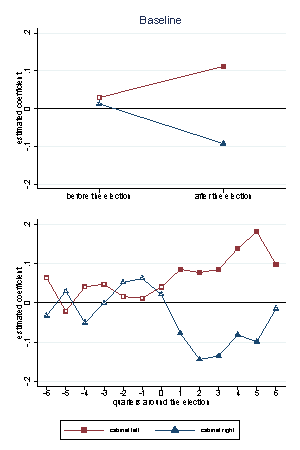
\includegraphics[width=\linewidth]{../results/applications/app_graphs_baseline.pdf}
%		{\scriptsize Note: These figures show the time evolution of refugee inflows as estimated in fixed effects regression with a set of dummies for before and after the election or a set of dummies for different quarters before and after an election in a quarter t = 0. Significant coefficients are indicated by filled plot markers. Periods in which the two coefficients are significantly different from each other are indicated with a grey background.\par}
%	\end{minipage}
%\end{figure}
%
%\clearpage
%\FloatBarrier
%\begin{table}[!ht]\centering \footnotesize
\def\sym#1{\ifmmode^{#1}\else\(^{#1}\)\fi}
\caption{Coefficients Graph 1 - baseline}
\begin{tabular}{l*{3}{c}}
\hline\hline
                   &\multicolumn{1}{c}{(1)}&\multicolumn{1}{c}{(2)}&\multicolumn{1}{c}{(3)}\\
                    &\multicolumn{1}{c}{left}&\multicolumn{1}{c}{right}&\multicolumn{1}{c}{diff}\\
\hline
before              &      0.0291         &      0.0128         &      0.0163         \\
                    &    (0.0244)         &    (0.0234)         &    (0.0340)         \\
[0.5em]
after               &       0.112\sym{***}&     -0.0929\sym{***}&       0.205\sym{***}\\
                    &    (0.0215)         &    (0.0226)         &    (0.0314)         \\
\hline
Observations        &       23705         &       23705         &       23705         \\
\hline\hline
\multicolumn{4}{l}{\footnotesize Standard errors in parentheses}\\
\multicolumn{4}{l}{\footnotesize \sym{*} \(p<0.05\), \sym{**} \(p<0.01\), \sym{***} \(p<0.001\)}\\
\end{tabular}
\end{table}

%\begin{table}[htbp]\centering
\def\sym#1{\ifmmode^{#1}\else\(^{#1}\)\fi}
\caption{Coefficients Graph 2}
\begin{tabular}{l*{2}{c}}
\hline\hline
                    &\multicolumn{1}{c}{(1)}&\multicolumn{1}{c}{(2)}\\
                    &\multicolumn{1}{c}{left}&\multicolumn{1}{c}{right}\\
\hline
 6 quarters before the election&      0.0555\sym{*}  &     -0.0244         \\
                    &    (0.0275)         &    (0.0365)         \\
[1em]
 5 quarters before the election&     -0.0294         &      0.0385         \\
                    &    (0.0295)         &    (0.0311)         \\
[1em]
 4 quarters before the election&      0.0333         &     -0.0422         \\
                    &    (0.0366)         &    (0.0385)         \\
[1em]
 3 quarters before the election&      0.0398         &     0.00650         \\
                    &    (0.0439)         &    (0.0302)         \\
[1em]
 2 quarters before the election&     0.00828         &      0.0600         \\
                    &    (0.0358)         &    (0.0385)         \\
[1em]
 1 quarters before the election&     0.00414         &      0.0701         \\
                    &    (0.0425)         &    (0.0363)         \\
[1em]
Quarter of the election&      0.0325         &      0.0293         \\
                    &    (0.0393)         &    (0.0374)         \\
[1em]
 1 quarters after the election&      0.0775\sym{*}  &     -0.0698         \\
                    &    (0.0373)         &    (0.0364)         \\
[1em]
 2 quarters after the election&      0.0697\sym{*}  &      -0.136\sym{***}\\
                    &    (0.0346)         &    (0.0338)         \\
[1em]
 3 quarters after the election&      0.0774\sym{*}  &      -0.127\sym{**} \\
                    &    (0.0339)         &    (0.0448)         \\
[1em]
 4 quarters after the election&       0.131\sym{***}&     -0.0733         \\
                    &    (0.0315)         &    (0.0384)         \\
[1em]
 5 quarters after the election&       0.173\sym{***}&     -0.0904\sym{**} \\
                    &    (0.0288)         &    (0.0350)         \\
[1em]
 6 quarters after the election&      0.0899\sym{***}&    -0.00688         \\
                    &    (0.0264)         &    (0.0296)         \\
\hline
Observations        &       23705         &       23705         \\
\hline\hline
\multicolumn{3}{l}{\footnotesize Standard errors in parentheses}\\
\multicolumn{3}{l}{\footnotesize \sym{*} \(p<0.05\), \sym{**} \(p<0.01\), \sym{***} \(p<0.001\)}\\
\end{tabular}
\end{table}

%
%
%\clearpage
%\FloatBarrier
%\begin{figure}[!ht]
%	\caption{First-time asylum applications per capita: predicted pattern - R1 to R6}
%	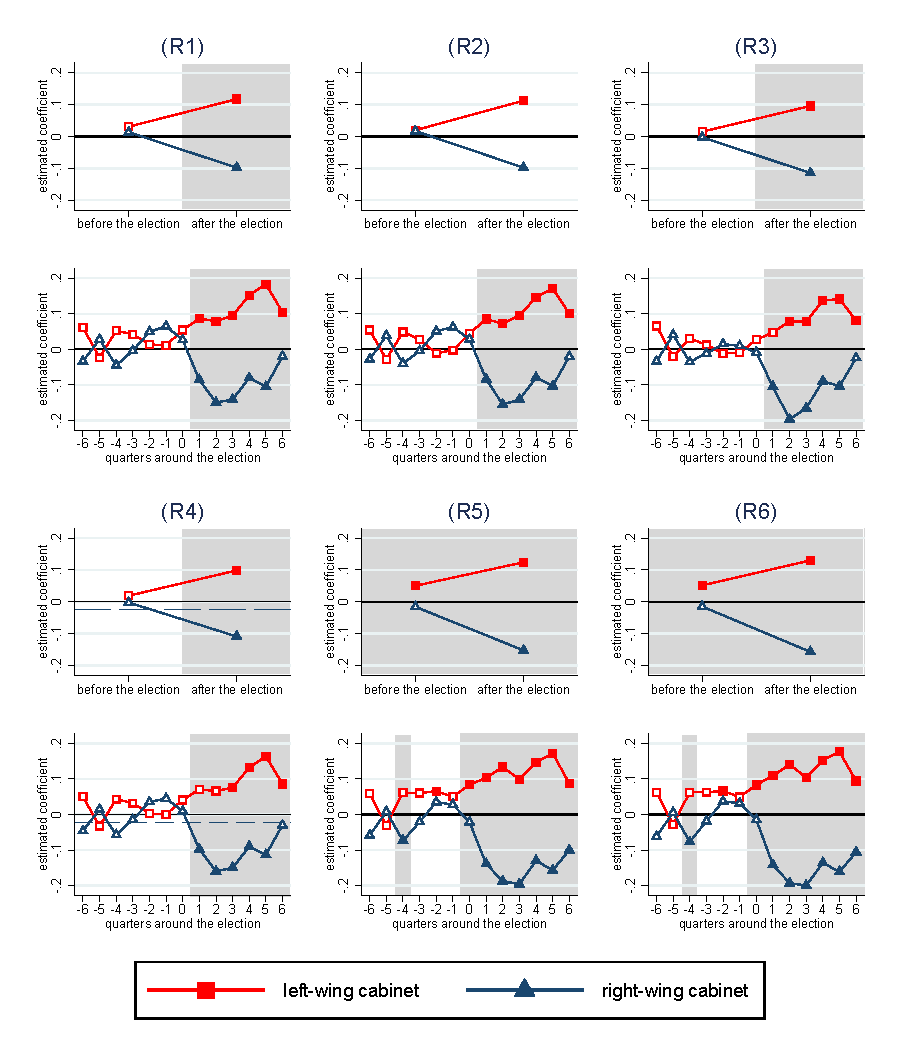
\includegraphics[width=1\textwidth]{../results/applications/app_graphs_R1-R6.pdf}
%	\scriptsize{Note: These figures show the time evolution of refugee inflows as estimated in fixed effects regression with a set of dummies for before and after the election or a set of dummies for different quarters before and after an election in a quarter t = 0. Significant coefficients are indicated by filled plot markers. Periods in which the two coefficients are significantly different from each other are indicated with a grey background. The navy dashed line in sub-figure R4 shows the average inflow of asylum seekers under right-wing cabinets in periods outside the election period. Significance of the coefficients of the right-wing cabinet in sub-figure R4 is reported for the distance to this average non-election period effect.}
%\end{figure}
%
%\clearpage
%\FloatBarrier
%
%\begin{table}[!ht]\centering \footnotesize
\def\sym#1{\ifmmode^{#1}\else\(^{#1}\)\fi}
\caption{Coefficients before after model - R1 - R2}
\begin{tabular}{l*{6}{c}}
\hline\hline
                    &\multicolumn{3}{c}{(R1)}&\multicolumn{3}{c}{(R2)}\\
                    &\multicolumn{1}{c}{left}&\multicolumn{1}{c}{right}&\multicolumn{1}{c}{diff}&\multicolumn{1}{c}{left}&\multicolumn{1}{c}{right}&\multicolumn{1}{c}{diff}\\
\hline
before              &      0.0295         &      0.0153         &      0.0143         &      0.0185         &      0.0189         &   -0.000336         \\
                    &    (0.0243)         &    (0.0233)         &    (0.0340)         &    (0.0250)         &    (0.0231)         &    (0.0346)         \\
[0.5em]
after               &       0.119\sym{***}&     -0.0948\sym{***}&       0.214\sym{***}&       0.114\sym{***}&     -0.0948\sym{***}&       0.209\sym{***}\\
                    &    (0.0226)         &    (0.0233)         &    (0.0332)         &    (0.0228)         &    (0.0230)         &    (0.0334)         \\
\hline
Observations        &       23705         &       23705         &       23705         &       23705         &       23705         &       23705         \\
\hline\hline
\multicolumn{7}{l}{ Standard errors in parentheses \sym{*} \(p<0.05\), \sym{**} \(p<0.01\), \sym{***} \(p<0.001\)}\\
\end{tabular}
\end{table}

%\begin{table}[!ht]\centering \footnotesize
\def\sym#1{\ifmmode^{#1}\else\(^{#1}\)\fi}
\caption{Coefficients quarterly model - R1 - R2}
\begin{tabular}{l*{6}{c}}
\hline\hline
                    &\multicolumn{3}{c}{(R1)}&\multicolumn{3}{c}{(R2)}\\
                    &\multicolumn{1}{c}{left}&\multicolumn{1}{c}{right}&\multicolumn{1}{c}{diff}&\multicolumn{1}{c}{left}&\multicolumn{1}{c}{right}&\multicolumn{1}{c}{diff}\\
\hline
 6 quarters before the election&      0.0646         &     -0.0313         &      0.0959         &      0.0572         &     -0.0259         &      0.0830         \\
                    &    (0.0350)         &    (0.0410)         &    (0.0642)         &    (0.0362)         &    (0.0407)         &    (0.0658)         \\
[0.5em]
 5 quarters before the election&     -0.0231         &      0.0320         &     -0.0551         &     -0.0271         &      0.0430         &     -0.0701         \\
                    &    (0.0316)         &    (0.0343)         &    (0.0541)         &    (0.0315)         &    (0.0328)         &    (0.0529)         \\
[0.5em]
 4 quarters before the election&      0.0409         &     -0.0499         &      0.0908         &      0.0375         &     -0.0447         &      0.0822         \\
                    &    (0.0341)         &    (0.0369)         &    (0.0508)         &    (0.0345)         &    (0.0360)         &    (0.0506)         \\
[0.5em]
 3 quarters before the election&      0.0475         &    -0.00320         &      0.0507         &      0.0328         &    -0.00366         &      0.0364         \\
                    &    (0.0416)         &    (0.0303)         &    (0.0512)         &    (0.0429)         &    (0.0303)         &    (0.0521)         \\
[0.5em]
 2 quarters before the election&      0.0171         &      0.0540         &     -0.0370         &    -0.00771         &      0.0561         &     -0.0638         \\
                    &    (0.0338)         &    (0.0371)         &    (0.0463)         &    (0.0337)         &    (0.0370)         &    (0.0447)         \\
[0.5em]
 1 quarters before the election&      0.0126         &      0.0698\sym{*}  &     -0.0572         &    -0.00144         &      0.0674\sym{*}  &     -0.0689         \\
                    &    (0.0361)         &    (0.0343)         &    (0.0420)         &    (0.0362)         &    (0.0338)         &    (0.0420)         \\
[0.5em]
Quarter of the election&      0.0438         &      0.0263         &      0.0175         &      0.0342         &      0.0285         &     0.00571         \\
                    &    (0.0356)         &    (0.0387)         &    (0.0497)         &    (0.0362)         &    (0.0383)         &    (0.0522)         \\
[0.5em]
 1 quarters after the election&      0.0912\sym{*}  &     -0.0780\sym{*}  &       0.169\sym{***}&      0.0892\sym{*}  &     -0.0765\sym{*}  &       0.166\sym{***}\\
                    &    (0.0389)         &    (0.0320)         &    (0.0455)         &    (0.0396)         &    (0.0315)         &    (0.0460)         \\
[0.5em]
 2 quarters after the election&      0.0803\sym{**} &      -0.146\sym{***}&       0.226\sym{***}&      0.0735\sym{*}  &      -0.151\sym{***}&       0.225\sym{***}\\
                    &    (0.0304)         &    (0.0353)         &    (0.0427)         &    (0.0298)         &    (0.0361)         &    (0.0440)         \\
[0.5em]
 3 quarters after the election&      0.0947\sym{**} &      -0.138\sym{***}&       0.233\sym{***}&      0.0948\sym{**} &      -0.138\sym{***}&       0.233\sym{***}\\
                    &    (0.0331)         &    (0.0398)         &    (0.0553)         &    (0.0332)         &    (0.0376)         &    (0.0542)         \\
[0.5em]
 4 quarters after the election&       0.149\sym{***}&     -0.0835\sym{*}  &       0.232\sym{***}&       0.142\sym{***}&     -0.0823\sym{*}  &       0.225\sym{***}\\
                    &    (0.0290)         &    (0.0354)         &    (0.0477)         &    (0.0298)         &    (0.0363)         &    (0.0495)         \\
[0.5em]
 5 quarters after the election&       0.190\sym{***}&      -0.102\sym{**} &       0.292\sym{***}&       0.178\sym{***}&      -0.100\sym{**} &       0.278\sym{***}\\
                    &    (0.0297)         &    (0.0358)         &    (0.0472)         &    (0.0296)         &    (0.0356)         &    (0.0474)         \\
[0.5em]
 6 quarters after the election&       0.106\sym{**} &     -0.0164         &       0.122\sym{*}  &       0.101\sym{**} &     -0.0168         &       0.118\sym{*}  \\
                    &    (0.0322)         &    (0.0317)         &    (0.0492)         &    (0.0322)         &    (0.0311)         &    (0.0479)         \\
\hline
Observations        &       23705         &       23705         &       23705         &       23705         &       23705         &       23705         \\
\hline\hline
\multicolumn{7}{l}{ Standard errors in parentheses \sym{*} \(p<0.05\), \sym{**} \(p<0.01\), \sym{***} \(p<0.001\)}\\
\end{tabular}
\end{table}

%\clearpage
%\FloatBarrier
%\begin{table}[!ht]\centering \footnotesize
\def\sym#1{\ifmmode^{#1}\else\(^{#1}\)\fi}
\caption{Coefficients before after model - R3 - R4}
\begin{tabular}{l*{6}{c}}
\hline\hline
                    &\multicolumn{3}{c}{(R3)}&\multicolumn{3}{c}{(R4)}\\
&\multicolumn{1}{c}{left}&\multicolumn{1}{c}{right}&\multicolumn{1}{c}{diff}&\multicolumn{1}{c}{left}&\multicolumn{1}{c}{right}&\multicolumn{1}{c}{diff}\\
\hline
before              &      0.0143         &    -0.00105         &      0.0153         &      0.0194         &      0.0223         &      0.0177         \\
                    &    (0.0239)         &    (0.0235)         &    (0.0335)         &    (0.0267)         &    (0.0223)         &    (0.0358)         \\
[0.5em]
after               &      0.0969\sym{***}&      -0.112\sym{***}&       0.209\sym{***}&       0.102\sym{***}&     -0.0831\sym{**} &       0.206\sym{***}\\
                    &    (0.0206)         &    (0.0229)         &    (0.0308)         &    (0.0229)         &    (0.0258)         &    (0.0325)         \\
\hline
Observations        &       23705         &       23705         &       23705         &       23705         &       23705         &       23705         \\
\hline\hline
\multicolumn{7}{l}{ Standard errors in parentheses \sym{*} \(p<0.05\), \sym{**} \(p<0.01\), \sym{***} \(p<0.001\)}\\
\end{tabular}
\end{table}

%\begin{table}[!ht]\centering \footnotesize
\def\sym#1{\ifmmode^{#1}\else\(^{#1}\)\fi}
\caption{Coefficients quarterly model - R3 - R4}
\begin{tabular}{l*{6}{c}}
\hline\hline
                    &\multicolumn{1}{c}{(1)}&\multicolumn{1}{c}{(2)}&\multicolumn{1}{c}{(3)}&\multicolumn{1}{c}{(4)}&\multicolumn{1}{c}{(5)}&\multicolumn{1}{c}{(6)}\\
                    &\multicolumn{1}{c}{left2\_R3}&\multicolumn{1}{c}{right2\_R3}&\multicolumn{1}{c}{diff2\_R3}&\multicolumn{1}{c}{left2\_R4}&\multicolumn{1}{c}{right2\_R4}&\multicolumn{1}{c}{diff2\_R4}\\
\hline
 6 quarters before the election&      0.0652         &     -0.0339         &      0.0991         &      0.0501         &     -0.0248         &      0.0963         \\
                    &    (0.0338)         &    (0.0418)         &    (0.0639)         &    (0.0274)         &    (0.0365)         &    (0.0649)         \\
[1em]
 5 quarters before the election&     -0.0207         &      0.0405         &     -0.0611         &     -0.0324         &      0.0361         &     -0.0470         \\
                    &    (0.0316)         &    (0.0341)         &    (0.0538)         &    (0.0295)         &    (0.0311)         &    (0.0548)         \\
[1em]
 4 quarters before the election&      0.0303         &     -0.0357         &      0.0660         &      0.0433         &     -0.0354         &       0.100         \\
                    &    (0.0338)         &    (0.0364)         &    (0.0510)         &    (0.0365)         &    (0.0381)         &    (0.0522)         \\
[1em]
 3 quarters before the election&      0.0123         &     -0.0117         &      0.0240         &      0.0319         &     0.00719         &      0.0462         \\
                    &    (0.0409)         &    (0.0303)         &    (0.0517)         &    (0.0438)         &    (0.0302)         &    (0.0527)         \\
[1em]
 2 quarters before the election&     -0.0115         &      0.0147         &     -0.0263         &     0.00273         &      0.0566         &     -0.0324         \\
                    &    (0.0337)         &    (0.0367)         &    (0.0449)         &    (0.0361)         &    (0.0386)         &    (0.0467)         \\
[1em]
 1 quarters before the election&    -0.00969         &     0.00946         &     -0.0191         &    0.000695         &      0.0665         &     -0.0443         \\
                    &    (0.0362)         &    (0.0348)         &    (0.0418)         &    (0.0426)         &    (0.0364)         &    (0.0418)         \\
[1em]
Quarter of the election&      0.0271         &    -0.00884         &      0.0359         &      0.0410         &      0.0310         &      0.0315         \\
                    &    (0.0348)         &    (0.0383)         &    (0.0472)         &    (0.0390)         &    (0.0373)         &    (0.0510)         \\
[1em]
 1 quarters after the election&      0.0473         &      -0.105\sym{**} &       0.153\sym{***}&      0.0706         &     -0.0763\sym{*}  &       0.168\sym{***}\\
                    &    (0.0379)         &    (0.0329)         &    (0.0450)         &    (0.0371)         &    (0.0366)         &    (0.0468)         \\
[1em]
 2 quarters after the election&      0.0783\sym{**} &      -0.197\sym{***}&       0.275\sym{***}&      0.0660         &      -0.138\sym{***}&       0.225\sym{***}\\
                    &    (0.0290)         &    (0.0352)         &    (0.0418)         &    (0.0346)         &    (0.0339)         &    (0.0433)         \\
[1em]
 3 quarters after the election&      0.0777\sym{*}  &      -0.165\sym{***}&       0.243\sym{***}&      0.0754\sym{*}  &      -0.128\sym{**} &       0.225\sym{***}\\
                    &    (0.0318)         &    (0.0400)         &    (0.0536)         &    (0.0339)         &    (0.0449)         &    (0.0544)         \\
[1em]
 4 quarters after the election&       0.137\sym{***}&     -0.0895\sym{**} &       0.226\sym{***}&       0.132\sym{***}&     -0.0684         &       0.222\sym{***}\\
                    &    (0.0272)         &    (0.0345)         &    (0.0450)         &    (0.0314)         &    (0.0384)         &    (0.0464)         \\
[1em]
 5 quarters after the election&       0.142\sym{***}&      -0.104\sym{**} &       0.246\sym{***}&       0.164\sym{***}&     -0.0919\sym{**} &       0.277\sym{***}\\
                    &    (0.0266)         &    (0.0357)         &    (0.0452)         &    (0.0286)         &    (0.0350)         &    (0.0466)         \\
[1em]
 6 quarters after the election&      0.0802\sym{**} &     -0.0245         &       0.105\sym{*}  &      0.0861\sym{***}&    -0.00824         &       0.116\sym{*}  \\
                    &    (0.0293)         &    (0.0303)         &    (0.0461)         &    (0.0262)         &    (0.0296)         &    (0.0476)         \\
\hline
Observations        &       23705         &       23705         &       23705         &       23705         &       23705         &       23705         \\
\hline\hline
\multicolumn{7}{l}{\footnotesize Standard errors in parentheses}\\
\multicolumn{7}{l}{\footnotesize \sym{*} \(p<0.05\), \sym{**} \(p<0.01\), \sym{***} \(p<0.001\)}\\
\end{tabular}
\end{table}

%\clearpage
%\FloatBarrier
%\begin{table}[!ht]\centering \footnotesize
\def\sym#1{\ifmmode^{#1}\else\(^{#1}\)\fi}
\caption{Coefficients before after model R5 - R6}
\begin{tabular}{l*{6}{c}}
\hline\hline
                    &\multicolumn{3}{c}{(R5)}&\multicolumn{3}{c}{(R6)}\\
&\multicolumn{1}{c}{left}&\multicolumn{1}{c}{right}&\multicolumn{1}{c}{diff}&\multicolumn{1}{c}{left}&\multicolumn{1}{c}{right}&\multicolumn{1}{c}{diff}\\
\hline
before              &      0.0484\sym{*}  &     -0.0134         &      0.0619         &      0.0494\sym{*}  &     -0.0123         &      0.0617\sym{*}  \\
                    &    (0.0235)         &    (0.0232)         &    (0.0320)         &    (0.0229)         &    (0.0230)         &    (0.0305)         \\
[0.5em]
after               &       0.126\sym{***}&      -0.148\sym{***}&       0.274\sym{***}&       0.131\sym{***}&      -0.153\sym{***}&       0.284\sym{***}\\
                    &    (0.0217)         &    (0.0237)         &    (0.0328)         &    (0.0229)         &    (0.0247)         &    (0.0359)         \\
\hline
Observations        &       23705         &       23705         &       23705         &       23705         &       23705         &       23705         \\
\hline\hline
\multicolumn{7}{l}{ Standard errors in parentheses \sym{*} \(p<0.05\), \sym{**} \(p<0.01\), \sym{***} \(p<0.001\)}\\
\end{tabular}
\end{table}

%\begin{table}[!ht]\centering \footnotesize
\def\sym#1{\ifmmode^{#1}\else\(^{#1}\)\fi}
\caption{Coefficients quarterly model R5 - R6}
\begin{tabular}{l*{6}{c}}
\hline\hline
                     &\multicolumn{3}{c}{(R5)}&\multicolumn{3}{c}{(R6)}\\
 &\multicolumn{1}{c}{left}&\multicolumn{1}{c}{right}&\multicolumn{1}{c}{diff}&\multicolumn{1}{c}{left}&\multicolumn{1}{c}{right}&\multicolumn{1}{c}{diff}\\
 \hline
 6 quarters before the election&      0.0624         &     -0.0554         &       0.118         &      0.0658         &     -0.0580         &       0.124         \\
                    &    (0.0338)         &    (0.0414)         &    (0.0637)         &    (0.0348)         &    (0.0407)         &    (0.0638)         \\
[0.5em]
 5 quarters before the election&     -0.0301         &      0.0137         &     -0.0438         &     -0.0269         &      0.0115         &     -0.0385         \\
                    &    (0.0315)         &    (0.0346)         &    (0.0537)         &    (0.0311)         &    (0.0335)         &    (0.0517)         \\
[0.5em]
 4 quarters before the election&      0.0481         &     -0.0786\sym{*}  &       0.127\sym{*}  &      0.0481         &     -0.0819\sym{*}  &       0.130\sym{**} \\
                    &    (0.0339)         &    (0.0366)         &    (0.0497)         &    (0.0335)         &    (0.0358)         &    (0.0480)         \\
[0.5em]
 3 quarters before the election&      0.0667         &     -0.0195         &      0.0862         &      0.0692         &     -0.0170         &      0.0862         \\
                    &    (0.0407)         &    (0.0302)         &    (0.0497)         &    (0.0406)         &    (0.0296)         &    (0.0474)         \\
[0.5em]
 2 quarters before the election&      0.0693\sym{*}  &      0.0414         &      0.0279         &      0.0697\sym{*}  &      0.0436         &      0.0261         \\
                    &    (0.0323)         &    (0.0376)         &    (0.0437)         &    (0.0322)         &    (0.0380)         &    (0.0441)         \\
[0.5em]
 1 quarters before the election&      0.0513         &      0.0343         &      0.0171         &      0.0503         &      0.0382         &      0.0121         \\
                    &    (0.0354)         &    (0.0336)         &    (0.0389)         &    (0.0339)         &    (0.0336)         &    (0.0367)         \\
[0.5em]
Quarter of the election&      0.0712\sym{*}  &     -0.0204         &      0.0916\sym{*}  &      0.0703\sym{*}  &     -0.0140         &      0.0844         \\
                    &    (0.0347)         &    (0.0381)         &    (0.0463)         &    (0.0339)         &    (0.0376)         &    (0.0441)         \\
[0.5em]
 1 quarters after the election&       0.108\sym{**} &      -0.128\sym{***}&       0.237\sym{***}&       0.115\sym{**} &      -0.131\sym{***}&       0.246\sym{***}\\
                    &    (0.0387)         &    (0.0332)         &    (0.0457)         &    (0.0384)         &    (0.0336)         &    (0.0463)         \\
[0.5em]
 2 quarters after the election&       0.135\sym{***}&      -0.182\sym{***}&       0.318\sym{***}&       0.141\sym{***}&      -0.187\sym{***}&       0.329\sym{***}\\
                    &    (0.0320)         &    (0.0355)         &    (0.0445)         &    (0.0330)         &    (0.0361)         &    (0.0467)         \\
[0.5em]
 3 quarters after the election&      0.0985\sym{**} &      -0.191\sym{***}&       0.290\sym{***}&       0.104\sym{**} &      -0.195\sym{***}&       0.299\sym{***}\\
                    &    (0.0325)         &    (0.0395)         &    (0.0546)         &    (0.0332)         &    (0.0401)         &    (0.0562)         \\
[0.5em]
 4 quarters after the election&       0.143\sym{***}&      -0.133\sym{***}&       0.276\sym{***}&       0.148\sym{***}&      -0.138\sym{***}&       0.287\sym{***}\\
                    &    (0.0281)         &    (0.0354)         &    (0.0473)         &    (0.0293)         &    (0.0369)         &    (0.0505)         \\
[0.5em]
 5 quarters after the election&       0.180\sym{***}&      -0.152\sym{***}&       0.332\sym{***}&       0.185\sym{***}&      -0.157\sym{***}&       0.341\sym{***}\\
                    &    (0.0278)         &    (0.0365)         &    (0.0473)         &    (0.0290)         &    (0.0375)         &    (0.0501)         \\
[0.5em]
 6 quarters after the election&      0.0894\sym{**} &     -0.0954\sym{**} &       0.185\sym{***}&      0.0958\sym{**} &      -0.100\sym{**} &       0.196\sym{***}\\
                    &    (0.0300)         &    (0.0308)         &    (0.0467)         &    (0.0313)         &    (0.0319)         &    (0.0498)         \\
\hline
Observations        &       23705         &       23705         &       23705         &       23705         &       23705         &       23705         \\
\hline\hline
\multicolumn{7}{l}{ Standard errors in parentheses \sym{*} \(p<0.05\), \sym{**} \(p<0.01\), \sym{***} \(p<0.001\)}\\
\end{tabular}
\end{table}


\clearpage
\FloatBarrier
\begin{table}[htbp]\centering \footnotesize
\def\sym#1{\ifmmode^{#1}\else\(^{#1}\)\fi}
\caption{Determinants of first-time asylum applications per capita - R7 - R12}
\begin{tabular}{l*{6}{c}}
\hline\hline
	&\multicolumn{1}{c}{(1)}     &\multicolumn{1}{c}{(2)}       &\multicolumn{1}{c}{(3)}       &\multicolumn{1}{c}{(4)}    	&\multicolumn{1}{c}{(5)}  	&\multicolumn{1}{c}{(6)}   \\
                    &\multicolumn{1}{c}{R7}         &\multicolumn{1}{c}{R8}         &\multicolumn{1}{c}{R9}         &\multicolumn{1}{c}{R10}         &\multicolumn{1}{c}{R11}         &\multicolumn{1}{c}{R12}         \\
\hline
Political Terror Scale	&       0.400\sym{***}& 0.337\sym{***}    &       0.409\sym{***}&       0.400\sym{***}&       0.400\sym{***}&       0.404\sym{***}\\
                    	&    (0.0696)         &     (0.0616)                  &    (0.0696)         &    (0.0697)         &    (0.0450)         &    (0.0706)         \\
[0,5em]
Civic Liberty (FHI) 	&       0.142         &        0.129              &       0.176         &       0.175         &       0.175\sym{**} &       0.170         \\
                    	&     (0.127)         &        (0.123)             &     (0.129)         &     (0.131)         &    (0.0611)         &     (0.134)         \\
[0,5em]
Political Rights (FHI)	&      0.0633         &       0.0564                &      0.0450         &      0.0487         &      0.0487         &      0.0476         \\
                    	&    (0.0712)         &          (0.0670)           &    (0.0751)         &    (0.0752)         &    (0.0479)         &    (0.0758)         \\
[0,5em]
Quarterly civil war 	&       0.192\sym{***}&     0.160\sym{***}          &    0.126\sym{***}                 &       0.188\sym{***}&       0.188\sym{***}&       0.186\sym{***}\\
battle death (000s)     &    (0.0224)         &  (0.0221)                   &     (0.0139)                 &    (0.0234)         &    (0.0265)         &    (0.0236)         \\
[0,5em]
Log origin country 		&      -0.636\sym{***}&   -0.693\sym{***}                  &      -0.654\sym{***}&      -0.661\sym{***}&      -0.661\sym{***}&      -0.651\sym{***}\\
real GDP per capita     &     (0.158)         &     (0.149)                 &     (0.167)         &     (0.163)         &     (0.105)         &     (0.163)         \\
[0,5em]
Log destination country &      -1.484\sym{**} &      -1.447\sym{**} &      -1.464\sym{**} &      -1.470\sym{**} &      -1.470\sym{*}  &      -1.483\sym{**} \\
real GDP per capita     &     (0.443)         &     (0.439)         &     (0.440)         &     (0.440)         &     (0.608)         &     (0.443)         \\
[0,5em]
Quarterly unemployment &     -0.0714\sym{***}&     -0.0740\sym{***}&     -0.0744\sym{***}&     -0.0745\sym{***}&     -0.0745\sym{***}&     -0.0714\sym{***}\\
rate at destination    &    (0.0108)         &    (0.0108)         &    (0.0108)         &    (0.0108)         &    (0.0112)         &    (0.0108)         \\
[0,5em]
Years after 2007          &                     &                     &                     &       0.190         &                     &                     \\
                    &                     &                     &                     &     (0.183)         &                     &                     \\
[0,5em]
Cabinet position left * &      0.0357         &      0.0290         &      0.0288         &      0.0291         &      0.0291         &      0.0248         \\
Before the election                    &    (0.0245)         &    (0.0245)         &    (0.0244)         &    (0.0244)         &    (0.0301)         &    (0.0240)         \\
[0,5em]
Cabinet position left * &       0.115\sym{***}&       0.112\sym{***}&       0.112\sym{***}&       0.112\sym{***}&       0.112\sym{***}&      0.0993\sym{***}\\
After the election                    &    (0.0215)         &    (0.0216)         &    (0.0215)         &    (0.0215)         &    (0.0286)         &    (0.0220)         \\
[0,5em]
Cabinet position right * &     0.00861         &      0.0120         &      0.0128         &      0.0128         &      0.0128         &      0.0135         \\
Before the election                    &    (0.0234)         &    (0.0234)         &    (0.0235)         &    (0.0234)         &    (0.0302)         &    (0.0238)         \\
[0,5em]
Cabinet position right * &     -0.0945\sym{***}&     -0.0945\sym{***}&     -0.0923\sym{***}&     -0.0929\sym{***}&     -0.0929\sym{**} &     -0.0913\sym{***}\\
After the election                    &    (0.0225)         &    (0.0223)         &    (0.0227)         &    (0.0226)         &    (0.0303)         &    (0.0261)         \\
\hline
Observations        &       23705         &       23705         &       23705         &       23705         &       23705         &       23239         \\
Adjusted \(R^{2}\)  &       0.182         &       0.168         &       0.177         &       0.176         &       0.176         &       0.175         \\
Fixed Effects       &       D x O         &       D x O         &       D x O         &       D x O         &       D x O         &       D x O         \\
Destination dummies &          No         &          No         &          No         &          No         &          No         &          No         \\
Quarter-Year dummies&         Yes         &         Yes         &         Yes         &         Yes         &         Yes         &         Yes         \\
\hline\hline
\multicolumn{7}{l}{Standard errors in parentheses \sym{*} \(p<0.05\), \sym{**} \(p<0.01\), \sym{***} \(p<0.001\)}\\
\end{tabular}
\end{table}


\clearpage
\FloatBarrier
\begin{figure}[!ht]
	\caption{First-time asylum applications per capita: predicted pattern - R7 to R12}
	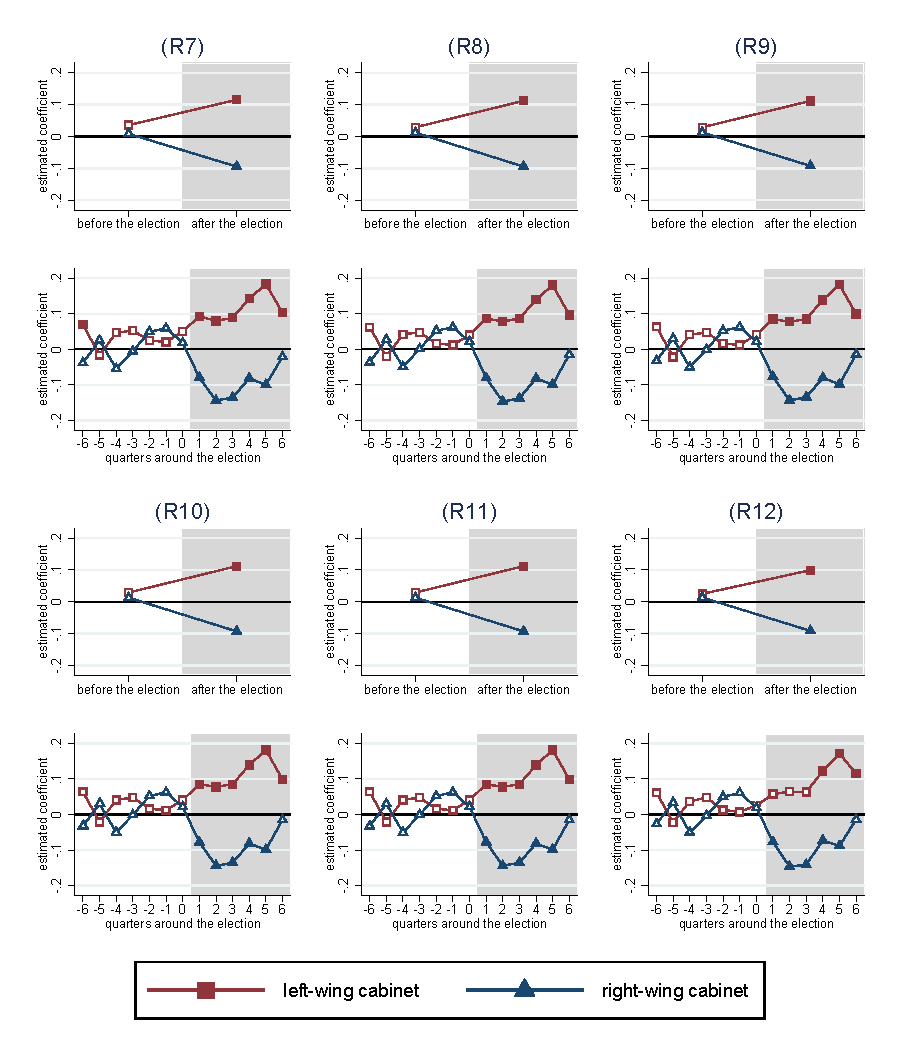
\includegraphics[width=1\textwidth]{../results/applications/app_graphs_R7-R12.pdf}
	\scriptsize{Note: These figures show the time evolution of refugee inflows as estimated in fixed effects regression
		with a set of dummies for before and after the election or a set of dummies for different quarters before and after an election in a quarter t = 0. Significant coefficients are indicated by filled plot markers. Periods in which the two coefficients are significantly different from each other are indicated with a grey background.}
\end{figure}

%
%\clearpage
%\FloatBarrier
%\begin{table}[!ht]\centering \footnotesize
\def\sym#1{\ifmmode^{#1}\else\(^{#1}\)\fi}
\caption{Coefficients before after model - R7 - R8}
\begin{tabular}{l*{6}{c}}
\hline\hline
                    &\multicolumn{1}{c}{(1)}&\multicolumn{1}{c}{(2)}&\multicolumn{1}{c}{(3)}&\multicolumn{1}{c}{(4)}&\multicolumn{1}{c}{(5)}&\multicolumn{1}{c}{(6)}\\
                    &\multicolumn{1}{c}{left1\_R7}&\multicolumn{1}{c}{right1\_R7}&\multicolumn{1}{c}{diff1\_R7}&\multicolumn{1}{c}{left1\_R8}&\multicolumn{1}{c}{right1\_R8}&\multicolumn{1}{c}{diff1\_R8}\\
\hline
before              &      0.0371         &     0.00683         &      0.0302         &      0.0304         &      0.0101         &      0.0203         \\
                    &    (0.0246)         &    (0.0234)         &    (0.0343)         &    (0.0246)         &    (0.0235)         &    (0.0341)         \\
[1em]
after               &       0.114\sym{***}&     -0.0977\sym{***}&       0.211\sym{***}&       0.110\sym{***}&     -0.0977\sym{***}&       0.208\sym{***}\\
                    &    (0.0213)         &    (0.0226)         &    (0.0314)         &    (0.0215)         &    (0.0224)         &    (0.0312)         \\
\hline
Observations        &       23705         &       23705         &       23705         &       23705         &       23705         &       23705         \\
\hline\hline
\multicolumn{7}{l}{\footnotesize Standard errors in parentheses}\\
\multicolumn{7}{l}{\footnotesize \sym{*} \(p<0.05\), \sym{**} \(p<0.01\), \sym{***} \(p<0.001\)}\\
\end{tabular}
\end{table}

%\begin{table}[!ht]\centering \footnotesize
\def\sym#1{\ifmmode^{#1}\else\(^{#1}\)\fi}
\caption{Coefficients quarterly model - R7 - R8}
\begin{tabular}{l*{6}{c}}
\hline\hline
                    &\multicolumn{1}{c}{(1)}&\multicolumn{1}{c}{(2)}&\multicolumn{1}{c}{(3)}&\multicolumn{1}{c}{(4)}&\multicolumn{1}{c}{(5)}&\multicolumn{1}{c}{(6)}\\
                    &\multicolumn{1}{c}{left2\_R7}&\multicolumn{1}{c}{right2\_R7}&\multicolumn{1}{c}{diff2\_R7}&\multicolumn{1}{c}{left2\_R8}&\multicolumn{1}{c}{right2\_R8}&\multicolumn{1}{c}{diff2\_R8}\\
\hline
 6 quarters before the election&      0.0660         &     -0.0407         &       0.107         &      0.0588         &     -0.0392         &      0.0980         \\
                    &    (0.0338)         &    (0.0417)         &    (0.0638)         &    (0.0342)         &    (0.0413)         &    (0.0637)         \\
[1em]
 5 quarters before the election&     -0.0177         &      0.0211         &     -0.0388         &     -0.0215         &      0.0231         &     -0.0446         \\
                    &    (0.0314)         &    (0.0347)         &    (0.0539)         &    (0.0318)         &    (0.0347)         &    (0.0544)         \\
[1em]
 4 quarters before the election&      0.0579         &     -0.0500         &       0.108\sym{*}  &      0.0540         &     -0.0450         &      0.0990         \\
                    &    (0.0342)         &    (0.0366)         &    (0.0513)         &    (0.0340)         &    (0.0364)         &    (0.0512)         \\
[1em]
 3 quarters before the election&      0.0472         &    -0.00654         &      0.0538         &      0.0413         &   -0.000311         &      0.0417         \\
                    &    (0.0414)         &    (0.0299)         &    (0.0517)         &    (0.0414)         &    (0.0302)         &    (0.0514)         \\
[1em]
 2 quarters before the election&      0.0209         &      0.0442         &     -0.0233         &      0.0130         &      0.0472         &     -0.0342         \\
                    &    (0.0339)         &    (0.0373)         &    (0.0457)         &    (0.0338)         &    (0.0369)         &    (0.0452)         \\
[1em]
 1 quarters before the election&      0.0192         &      0.0535         &     -0.0344         &      0.0104         &      0.0562         &     -0.0458         \\
                    &    (0.0366)         &    (0.0340)         &    (0.0415)         &    (0.0365)         &    (0.0341)         &    (0.0410)         \\
[1em]
Quarter of the election&      0.0600         &      0.0180         &      0.0419         &      0.0511         &      0.0210         &      0.0301         \\
                    &    (0.0361)         &    (0.0383)         &    (0.0499)         &    (0.0362)         &    (0.0384)         &    (0.0504)         \\
[1em]
 1 quarters after the election&      0.0879\sym{*}  &     -0.0876\sym{**} &       0.176\sym{***}&      0.0816\sym{*}  &     -0.0892\sym{**} &       0.171\sym{***}\\
                    &    (0.0387)         &    (0.0325)         &    (0.0451)         &    (0.0387)         &    (0.0325)         &    (0.0454)         \\
[1em]
 2 quarters after the election&      0.0780\sym{**} &      -0.148\sym{***}&       0.226\sym{***}&      0.0760\sym{*}  &      -0.151\sym{***}&       0.227\sym{***}\\
                    &    (0.0302)         &    (0.0352)         &    (0.0422)         &    (0.0308)         &    (0.0350)         &    (0.0420)         \\
[1em]
 3 quarters after the election&      0.0883\sym{**} &      -0.139\sym{***}&       0.227\sym{***}&      0.0865\sym{**} &      -0.141\sym{***}&       0.228\sym{***}\\
                    &    (0.0324)         &    (0.0392)         &    (0.0542)         &    (0.0322)         &    (0.0395)         &    (0.0541)         \\
[1em]
 4 quarters after the election&       0.146\sym{***}&     -0.0787\sym{*}  &       0.224\sym{***}&       0.142\sym{***}&     -0.0792\sym{*}  &       0.222\sym{***}\\
                    &    (0.0278)         &    (0.0345)         &    (0.0459)         &    (0.0282)         &    (0.0341)         &    (0.0458)         \\
[1em]
 5 quarters after the election&       0.176\sym{***}&      -0.103\sym{**} &       0.280\sym{***}&       0.174\sym{***}&      -0.103\sym{**} &       0.277\sym{***}\\
                    &    (0.0274)         &    (0.0357)         &    (0.0464)         &    (0.0279)         &    (0.0352)         &    (0.0463)         \\
[1em]
 6 quarters after the election&       0.101\sym{***}&     -0.0241         &       0.125\sym{**} &      0.0946\sym{**} &     -0.0179         &       0.113\sym{*}  \\
                    &    (0.0299)         &    (0.0304)         &    (0.0469)         &    (0.0304)         &    (0.0301)         &    (0.0471)         \\
\hline
Observations        &       23705         &       23705         &       23705         &       23705         &       23705         &       23705         \\
\hline\hline
\multicolumn{7}{l}{\footnotesize Standard errors in parentheses}\\
\multicolumn{7}{l}{\footnotesize \sym{*} \(p<0.05\), \sym{**} \(p<0.01\), \sym{***} \(p<0.001\)}\\
\end{tabular}
\end{table}

%\clearpage
%\FloatBarrier
%\begin{table}[!ht]\centering \footnotesize
\def\sym#1{\ifmmode^{#1}\else\(^{#1}\)\fi}
\caption{Coefficients before after model - R9 - R10}
\begin{tabular}{l*{6}{c}}
\hline\hline
                    &\multicolumn{1}{c}{(1)}&\multicolumn{1}{c}{(2)}&\multicolumn{1}{c}{(3)}&\multicolumn{1}{c}{(4)}&\multicolumn{1}{c}{(5)}&\multicolumn{1}{c}{(6)}\\
                    &\multicolumn{1}{c}{left1\_R9}&\multicolumn{1}{c}{right1\_R9}&\multicolumn{1}{c}{diff1\_R9}&\multicolumn{1}{c}{left1\_R10}&\multicolumn{1}{c}{right1\_R10}&\multicolumn{1}{c}{diff1\_R10}\\
\hline
before              &      0.0302         &      0.0110         &      0.0192         &      0.0304         &      0.0109         &      0.0195         \\
                    &    (0.0245)         &    (0.0235)         &    (0.0342)         &    (0.0245)         &    (0.0235)         &    (0.0342)         \\
[1em]
after               &       0.110\sym{***}&     -0.0956\sym{***}&       0.206\sym{***}&       0.110\sym{***}&     -0.0962\sym{***}&       0.206\sym{***}\\
                    &    (0.0213)         &    (0.0227)         &    (0.0315)         &    (0.0213)         &    (0.0226)         &    (0.0314)         \\
\hline
Observations        &       23705         &       23705         &       23705         &       23705         &       23705         &       23705         \\
\hline\hline
\multicolumn{7}{l}{\footnotesize Standard errors in parentheses}\\
\multicolumn{7}{l}{\footnotesize \sym{*} \(p<0.05\), \sym{**} \(p<0.01\), \sym{***} \(p<0.001\)}\\
\end{tabular}
\end{table}

%\begin{table}[!ht]\centering \footnotesize
\def\sym#1{\ifmmode^{#1}\else\(^{#1}\)\fi}
\caption{Coefficients quarterly model - R9 - R10}
\begin{tabular}{l*{6}{c}}
\hline\hline
                    &\multicolumn{3}{c}{(R9)}&\multicolumn{3}{c}{(R10)}\\
&\multicolumn{1}{c}{left}&\multicolumn{1}{c}{right}&\multicolumn{1}{c}{diff}&\multicolumn{1}{c}{left}&\multicolumn{1}{c}{right}&\multicolumn{1}{c}{diff}\\

\hline
 6 quarters before the election&      0.0630         &     -0.0325         &      0.0955         &      0.0638         &     -0.0326         &      0.0964         \\
                    &    (0.0342)         &    (0.0414)         &    (0.0640)         &    (0.0340)         &    (0.0415)         &    (0.0639)         \\
[0.5em]
 5 quarters before the election&     -0.0218         &      0.0301         &     -0.0520         &     -0.0213         &      0.0301         &     -0.0513         \\
                    &    (0.0314)         &    (0.0346)         &    (0.0538)         &    (0.0313)         &    (0.0346)         &    (0.0537)         \\
[0.5em]
 4 quarters before the election&      0.0407         &     -0.0504         &      0.0911         &      0.0411         &     -0.0504         &      0.0916         \\
                    &    (0.0340)         &    (0.0371)         &    (0.0510)         &    (0.0341)         &    (0.0370)         &    (0.0509)         \\
[0.5em]
 3 quarters before the election&      0.0473         &    -0.00110         &      0.0484         &      0.0477         &    -0.00112         &      0.0488         \\
                    &    (0.0414)         &    (0.0299)         &    (0.0513)         &    (0.0414)         &    (0.0299)         &    (0.0513)         \\
[0.5em]
 2 quarters before the election&      0.0160         &      0.0523         &     -0.0363         &      0.0161         &      0.0522         &     -0.0361         \\
                    &    (0.0336)         &    (0.0373)         &    (0.0454)         &    (0.0336)         &    (0.0373)         &    (0.0454)         \\
[0.5em]
 1 quarters before the election&      0.0123         &      0.0624         &     -0.0501         &      0.0122         &      0.0623         &     -0.0501         \\
                    &    (0.0363)         &    (0.0342)         &    (0.0412)         &    (0.0363)         &    (0.0342)         &    (0.0413)         \\
[0.5em]
Quarter of the election&      0.0408         &      0.0215         &      0.0193         &      0.0406         &      0.0215         &      0.0191         \\
                    &    (0.0361)         &    (0.0385)         &    (0.0497)         &    (0.0362)         &    (0.0385)         &    (0.0497)         \\
[0.5em]
 1 quarters after the election&      0.0852\sym{*}  &     -0.0775\sym{*}  &       0.163\sym{***}&      0.0853\sym{*}  &     -0.0777\sym{*}  &       0.163\sym{***}\\
                    &    (0.0390)         &    (0.0324)         &    (0.0452)         &    (0.0390)         &    (0.0324)         &    (0.0452)         \\
[0.5em]
 2 quarters after the election&      0.0771\sym{*}  &      -0.144\sym{***}&       0.221\sym{***}&      0.0775\sym{*}  &      -0.144\sym{***}&       0.222\sym{***}\\
                    &    (0.0304)         &    (0.0354)         &    (0.0423)         &    (0.0303)         &    (0.0353)         &    (0.0422)         \\
[0.5em]
 3 quarters after the election&      0.0849\sym{**} &      -0.135\sym{***}&       0.220\sym{***}&      0.0852\sym{**} &      -0.136\sym{***}&       0.221\sym{***}\\
                    &    (0.0324)         &    (0.0390)         &    (0.0537)         &    (0.0324)         &    (0.0391)         &    (0.0539)         \\
[0.5em]
 4 quarters after the election&       0.139\sym{***}&     -0.0805\sym{*}  &       0.219\sym{***}&       0.139\sym{***}&     -0.0814\sym{*}  &       0.220\sym{***}\\
                    &    (0.0278)         &    (0.0347)         &    (0.0461)         &    (0.0278)         &    (0.0345)         &    (0.0458)         \\
[0.5em]
 5 quarters after the election&       0.182\sym{***}&     -0.0982\sym{**} &       0.280\sym{***}&       0.181\sym{***}&     -0.0990\sym{**} &       0.280\sym{***}\\
                    &    (0.0276)         &    (0.0358)         &    (0.0468)         &    (0.0277)         &    (0.0356)         &    (0.0466)         \\
[0.5em]
 6 quarters after the election&      0.0989\sym{***}&     -0.0143         &       0.113\sym{*}  &      0.0985\sym{**} &     -0.0149         &       0.113\sym{*}  \\
                    &    (0.0300)         &    (0.0303)         &    (0.0467)         &    (0.0301)         &    (0.0302)         &    (0.0467)         \\
\hline
Observations        &       23705         &       23705         &       23705         &       23705         &       23705         &       23705         \\
\hline\hline
\multicolumn{7}{l}{ Standard errors in parentheses \sym{*} \(p<0.05\), \sym{**} \(p<0.01\), \sym{***} \(p<0.001\)}\\
\end{tabular}
\end{table}

%\clearpage
%\FloatBarrier
%\begin{table}[!ht]\centering \footnotesize
\def\sym#1{\ifmmode^{#1}\else\(^{#1}\)\fi}
\caption{Coefficients before after model R11 - R12}
\begin{tabular}{l*{6}{c}}
\hline\hline
                    &\multicolumn{3}{c}{(R11)}&\multicolumn{3}{c}{(R12)}\\
&\multicolumn{1}{c}{left}&\multicolumn{1}{c}{right}&\multicolumn{1}{c}{diff}&\multicolumn{1}{c}{left}&\multicolumn{1}{c}{right}&\multicolumn{1}{c}{diff}\\
\hline
before              &      0.0291         &      0.0128         &      0.0163         &      0.0248         &      0.0135         &      0.0113         \\
                    &    (0.0301)         &    (0.0302)         &    (0.0473)         &    (0.0240)         &    (0.0238)         &    (0.0335)         \\
[0.5em]
after               &       0.112\sym{***}&     -0.0929\sym{**} &       0.205\sym{***}&      0.0993\sym{***}&     -0.0913\sym{***}&       0.191\sym{***}\\
                    &    (0.0286)         &    (0.0303)         &    (0.0436)         &    (0.0220)         &    (0.0261)         &    (0.0332)         \\
\hline
Observations        &       23705         &       23705         &       23705         &       23239         &       23239         &       23239         \\
\hline\hline
\multicolumn{7}{l}{ Standard errors in parentheses \sym{*} \(p<0.05\), \sym{**} \(p<0.01\), \sym{***} \(p<0.001\)}\\
\end{tabular}
\end{table}

%\begin{table}[!ht]\centering \footnotesize
\def\sym#1{\ifmmode^{#1}\else\(^{#1}\)\fi}
\caption{Coefficients quarterly model R11 - R12}
\begin{tabular}{l*{6}{c}}
\hline\hline
                    &\multicolumn{1}{c}{(1)}&\multicolumn{1}{c}{(2)}&\multicolumn{1}{c}{(3)}&\multicolumn{1}{c}{(4)}&\multicolumn{1}{c}{(5)}&\multicolumn{1}{c}{(6)}\\
                    &\multicolumn{1}{c}{left2\_R11}&\multicolumn{1}{c}{right2\_R11}&\multicolumn{1}{c}{diff2\_R11}&\multicolumn{1}{c}{left2\_R12}&\multicolumn{1}{c}{right2\_R12}&\multicolumn{1}{c}{diff2\_R12}\\
\hline
 6 quarters before the election&      0.0605         &     -0.0350         &      0.0955         &      0.0578         &     -0.0297         &      0.0875         \\
                    &    (0.0395)         &    (0.0407)         &    (0.0629)         &    (0.0322)         &    (0.0417)         &    (0.0626)         \\
[1em]
 5 quarters before the election&     -0.0222         &      0.0256         &     -0.0479         &     -0.0227         &      0.0288         &     -0.0515         \\
                    &    (0.0386)         &    (0.0404)         &    (0.0632)         &    (0.0306)         &    (0.0346)         &    (0.0533)         \\
[1em]
 4 quarters before the election&      0.0530         &     -0.0457         &      0.0987         &      0.0488         &     -0.0456         &      0.0945         \\
                    &    (0.0433)         &    (0.0425)         &    (0.0625)         &    (0.0340)         &    (0.0364)         &    (0.0505)         \\
[1em]
 3 quarters before the election&      0.0418         &    -0.00232         &      0.0442         &      0.0417         &    -0.00478         &      0.0464         \\
                    &    (0.0491)         &    (0.0463)         &    (0.0686)         &    (0.0420)         &    (0.0305)         &    (0.0524)         \\
[1em]
 2 quarters before the election&      0.0125         &      0.0468         &     -0.0343         &     0.00869         &      0.0443         &     -0.0356         \\
                    &    (0.0434)         &    (0.0454)         &    (0.0636)         &    (0.0336)         &    (0.0378)         &    (0.0451)         \\
[1em]
 1 quarters before the election&      0.0108         &      0.0569         &     -0.0461         &     0.00624         &      0.0553         &     -0.0491         \\
                    &    (0.0400)         &    (0.0426)         &    (0.0611)         &    (0.0370)         &    (0.0344)         &    (0.0416)         \\
[1em]
Quarter of the election&      0.0512         &      0.0213         &      0.0299         &      0.0372         &      0.0196         &      0.0176         \\
                    &    (0.0374)         &    (0.0405)         &    (0.0558)         &    (0.0372)         &    (0.0384)         &    (0.0491)         \\
[1em]
 1 quarters after the election&      0.0804\sym{*}  &     -0.0861\sym{*}  &       0.167\sym{**} &      0.0522         &     -0.0857\sym{*}  &       0.138\sym{**} \\
                    &    (0.0370)         &    (0.0394)         &    (0.0509)         &    (0.0396)         &    (0.0348)         &    (0.0436)         \\
[1em]
 2 quarters after the election&      0.0758\sym{*}  &      -0.148\sym{***}&       0.224\sym{***}&      0.0619         &      -0.151\sym{***}&       0.213\sym{***}\\
                    &    (0.0375)         &    (0.0412)         &    (0.0555)         &    (0.0335)         &    (0.0369)         &    (0.0454)         \\
[1em]
 3 quarters after the election&      0.0852\sym{*}  &      -0.139\sym{**} &       0.224\sym{***}&      0.0636\sym{*}  &      -0.146\sym{**} &       0.209\sym{***}\\
                    &    (0.0392)         &    (0.0429)         &    (0.0603)         &    (0.0322)         &    (0.0447)         &    (0.0564)         \\
[1em]
 4 quarters after the election&       0.142\sym{***}&     -0.0786         &       0.221\sym{***}&       0.127\sym{***}&     -0.0709         &       0.198\sym{***}\\
                    &    (0.0387)         &    (0.0433)         &    (0.0586)         &    (0.0287)         &    (0.0401)         &    (0.0500)         \\
[1em]
 5 quarters after the election&       0.174\sym{***}&      -0.103\sym{*}  &       0.277\sym{***}&       0.164\sym{***}&     -0.0928\sym{*}  &       0.257\sym{***}\\
                    &    (0.0384)         &    (0.0415)         &    (0.0592)         &    (0.0279)         &    (0.0380)         &    (0.0486)         \\
[1em]
 6 quarters after the election&      0.0968\sym{*}  &     -0.0183         &       0.115         &       0.111\sym{***}&     -0.0164         &       0.127\sym{**} \\
                    &    (0.0385)         &    (0.0374)         &    (0.0600)         &    (0.0307)         &    (0.0332)         &    (0.0478)         \\
\hline
Observations        &       23705         &       23705         &       23705         &       23239         &       23239         &       23239         \\
\hline\hline
\multicolumn{7}{l}{\footnotesize Standard errors in parentheses}\\
\multicolumn{7}{l}{\footnotesize \sym{*} \(p<0.05\), \sym{**} \(p<0.01\), \sym{***} \(p<0.001\)}\\
\end{tabular}
\end{table}



\clearpage
\FloatBarrier
\begin{table}[htbp]\centering \scriptsize
\def\sym#1{\ifmmode^{#1}\else\(^{#1}\)\fi}
\caption{Determinants of first-time asylum applications per capita - R13 - R18}
\begin{tabular}{l*{6}{c}}
\hline\hline
	&\multicolumn{1}{c}{(1)}     &\multicolumn{1}{c}{(2)}       &\multicolumn{1}{c}{(3)}       &\multicolumn{1}{c}{(4)}    	&\multicolumn{1}{c}{(5)}  	&\multicolumn{1}{c}{(6)}   \\
                    &\multicolumn{1}{c}{R13}         &\multicolumn{1}{c}{R14}         &\multicolumn{1}{c}{R15}         &\multicolumn{1}{c}{R16}         &\multicolumn{1}{c}{R17}         &\multicolumn{1}{c}{R18}         \\
\hline
Political Terror Scale&       0.400\sym{***}&       0.400\sym{***}&       0.374\sym{***}&       0.414\sym{***}&       0.404\sym{***}&       0.410\sym{***}\\
                    &    (0.0450)         &    (0.0450)         &    (0.0657)         &    (0.0750)         &    (0.0785)         &    (0.0849)         \\
[0.5em]
Civic Liberty (FHI) &       0.175\sym{**} &       0.176\sym{**} &       0.166         &       0.195         &       0.163         &       0.172         \\
                    &    (0.0611)         &    (0.0612)         &     (0.124)         &     (0.133)         &     (0.132)         &     (0.143)         \\
[0.5em]
Political Rights (FHI)&      0.0483         &      0.0478         &      0.0396         &      0.0420         &      0.0450         &      0.0513         \\
                    &    (0.0478)         &    (0.0478)         &    (0.0689)         &    (0.0797)         &    (0.0759)         &    (0.0785)         \\
[0.5em]
Quarterly civil war&       0.188\sym{***}&       0.187\sym{***}&       0.191\sym{***}&       0.201\sym{***}&       0.207\sym{***}&       0.186\sym{***}\\
 battle death (000s)                    &    (0.0265)         &    (0.0265)         &    (0.0226)         &    (0.0249)         &    (0.0263)         &    (0.0232)         \\
[0.5em]
Log origin country &      -0.662\sym{***}&      -0.663\sym{***}&      -0.633\sym{***}&      -0.641\sym{***}&      -0.571\sym{**} &      -0.766\sym{***}\\
real GDP per capita                   &     (0.105)         &     (0.105)         &     (0.150)         &     (0.160)         &     (0.163)         &     (0.170)         \\
[0.5em]
Log destination country &      -1.466\sym{*}  &      -1.513\sym{*}  &      -1.246\sym{**} &      -1.353\sym{*}  &      -0.102         &      -1.771\sym{***}\\
quarterly real GDP per capita                    &     (0.613)         &     (0.608)         &     (0.411)         &     (0.524)         &     (0.530)         &     (0.471)         \\
[0.5em]
Quarterly unemployment &     -0.0728\sym{***}&     -0.0736\sym{***}&     -0.0631\sym{***}&     -0.0739\sym{***}&    -0.00992         &     -0.0737\sym{***}\\
rate at destination                    &    (0.0111)         &    (0.0111)         &   (0.00955)         &    (0.0115)         &    (0.0104)         &    (0.0112)         \\
[0.5em]
Log average total first-time &                     &                     &                     &                     &       0.728\sym{***}&                     \\
applications in the previous 6 quarters                    &                     &                     &                     &                     &    (0.0524)         &                     \\
[0.5em]
Cabinet position left * &      0.0115         &      0.0143         &      0.0305         &      0.0128         &    -0.00704         &      0.0364         \\
Before the election                    &    (0.0297)         &    (0.0321)         &    (0.0229)         &    (0.0250)         &    (0.0237)         &    (0.0324)         \\
[0.5em]
Cabinet position left * &       0.104\sym{***}&       0.112\sym{***}&       0.108\sym{***}&       0.105\sym{***}&      0.0487\sym{*}  &       0.195\sym{***}\\
After the election                    &    (0.0280)         &    (0.0337)         &    (0.0203)         &    (0.0206)         &    (0.0185)         &    (0.0316)         \\
[0.5em]
Cabinet position right * &      0.0318         &      0.0322         &     0.00798         &      0.0209         &     -0.0141         &      0.0306         \\
Before the election                   &    (0.0303)         &    (0.0280)         &    (0.0213)         &    (0.0257)         &    (0.0251)         &    (0.0305)         \\
[0.5em]
Cabinet position right * &     -0.0806\sym{**} &     -0.0424         &     -0.0763\sym{**} &     -0.0992\sym{***}&     -0.0566\sym{*}  &     -0.0419         \\
After the election                    &    (0.0287)         &    (0.0276)         &    (0.0226)         &    (0.0238)         &    (0.0241)         &    (0.0319)         \\
\hline
Observations        &       23705         &       23705         &       25466         &       22446         &       22391         &       16488         \\
Adjusted \(R^{2}\)  &       0.176         &       0.175         &       0.162         &       0.185         &       0.250         &       0.183         \\
Fixed Effects       &       D x O         &       D x O         &       D x O         &       D x O         &       D x O         &       D x O         \\
Destination dummies &          No         &          No         &          No         &          No         &          No         &          No         \\
Quarter-Year dummies&         Yes         &         Yes         &         Yes         &         Yes         &         Yes         &         Yes         \\
\hline\hline
\multicolumn{7}{l}{ Standard errors in parentheses \sym{*} \(p<0.05\), \sym{**} \(p<0.01\), \sym{***} \(p<0.001\)}\\
\end{tabular}
\end{table}


\clearpage
\FloatBarrier
\begin{figure}[!ht]
	\caption{First-time asylum applications per capita: predicted pattern - R13 to R18}
	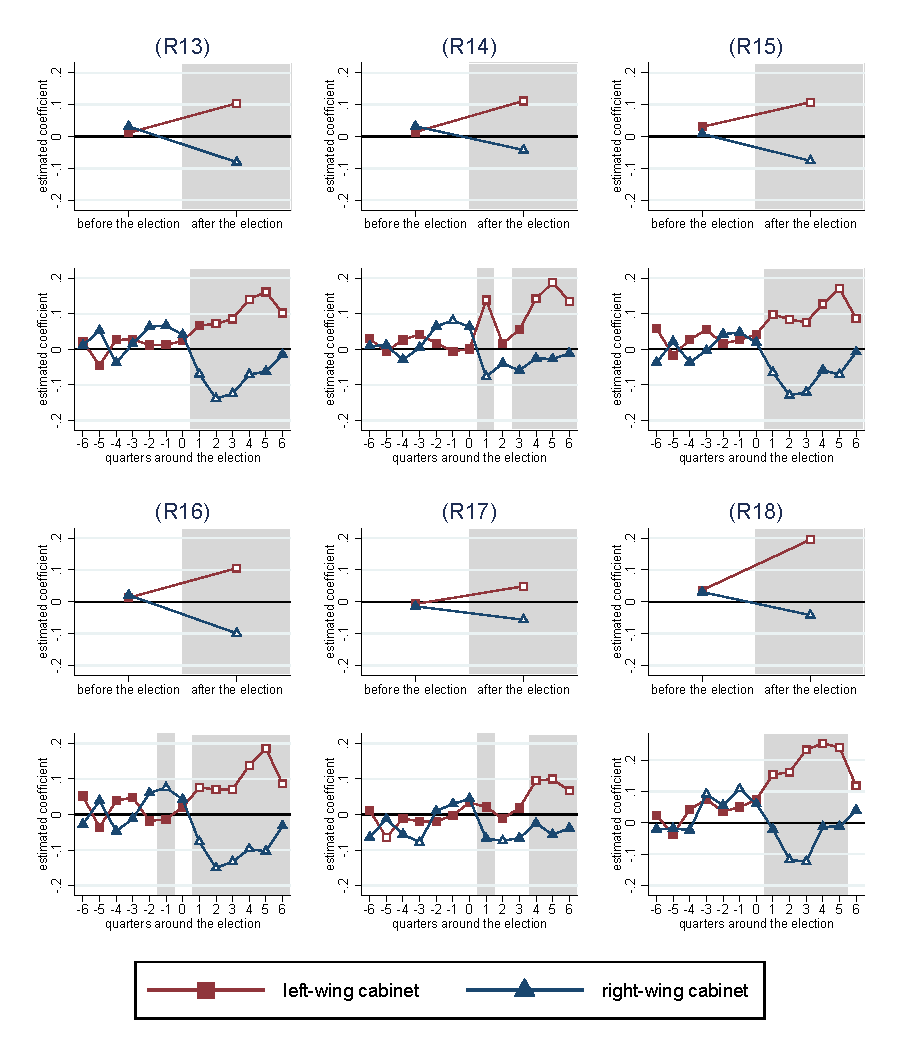
\includegraphics[width=1\textwidth]{../results/applications/app_graphs_R13-R18.pdf}
	\scriptsize{Note: These figures show the time evolution of refugee inflows as estimated in fixed effects regression
		with a set of dummies for before and after the election or a set of dummies for different quarters before and after an election in a quarter t = 0. Significant coefficients are indicated by filled plot markers. Periods in which the two coefficients are significantly different from each other are indicated with a grey background.}
\end{figure}

%\clearpage
%\FloatBarrier
%\begin{table}[!ht]\centering \footnotesize
\def\sym#1{\ifmmode^{#1}\else\(^{#1}\)\fi}
\caption{Coefficients before after model - R13 - R14}
\begin{tabular}{l*{6}{c}}
\hline\hline
                    &\multicolumn{1}{c}{(1)}&\multicolumn{1}{c}{(2)}&\multicolumn{1}{c}{(3)}&\multicolumn{1}{c}{(4)}&\multicolumn{1}{c}{(5)}&\multicolumn{1}{c}{(6)}\\
                    &\multicolumn{1}{c}{left1\_R13}&\multicolumn{1}{c}{right1\_R13}&\multicolumn{1}{c}{diff1\_R13}&\multicolumn{1}{c}{left1\_R14}&\multicolumn{1}{c}{right1\_R14}&\multicolumn{1}{c}{diff1\_R14}\\
\hline
before              &      0.0127         &      0.0302         &     -0.0175         &      0.0139         &      0.0323         &     -0.0183         \\
                    &    (0.0249)         &    (0.0232)         &    (0.0342)         &    (0.0273)         &    (0.0188)         &    (0.0315)         \\
[1em]
after               &       0.102\sym{***}&     -0.0834\sym{***}&       0.186\sym{***}&       0.110\sym{***}&     -0.0454\sym{*}  &       0.156\sym{***}\\
                    &    (0.0215)         &    (0.0207)         &    (0.0291)         &    (0.0232)         &    (0.0208)         &    (0.0312)         \\
\hline
Observations        &       23705         &       23705         &       23705         &       23705         &       23705         &       23705         \\
\hline\hline
\multicolumn{7}{l}{\footnotesize Standard errors in parentheses}\\
\multicolumn{7}{l}{\footnotesize \sym{*} \(p<0.05\), \sym{**} \(p<0.01\), \sym{***} \(p<0.001\)}\\
\end{tabular}
\end{table}

%\begin{table}[!ht]\centering \footnotesize
\def\sym#1{\ifmmode^{#1}\else\(^{#1}\)\fi}
\caption{Coefficients quarterly model - R13 - R14}
\begin{tabular}{l*{6}{c}}
\hline\hline
                    &\multicolumn{1}{c}{(1)}&\multicolumn{1}{c}{(2)}&\multicolumn{1}{c}{(3)}&\multicolumn{1}{c}{(4)}&\multicolumn{1}{c}{(5)}&\multicolumn{1}{c}{(6)}\\
                    &\multicolumn{1}{c}{left2\_R13}&\multicolumn{1}{c}{right2\_R13}&\multicolumn{1}{c}{diff2\_R13}&\multicolumn{1}{c}{left2\_R14}&\multicolumn{1}{c}{right2\_R14}&\multicolumn{1}{c}{diff2\_R14}\\
\hline
 6 quarters before the election&      0.0192         &     0.00723         &      0.0120         &      0.0265         &     0.00628         &      0.0202         \\
                    &    (0.0352)         &    (0.0391)         &    (0.0624)         &    (0.0374)         &    (0.0305)         &    (0.0544)         \\
[1em]
 5 quarters before the election&     -0.0466         &      0.0484         &     -0.0950         &     -0.0115         &      0.0108         &     -0.0222         \\
                    &    (0.0340)         &    (0.0326)         &    (0.0546)         &    (0.0361)         &    (0.0286)         &    (0.0516)         \\
[1em]
 4 quarters before the election&      0.0380         &     -0.0335         &      0.0715         &      0.0361         &     -0.0234         &      0.0595         \\
                    &    (0.0337)         &    (0.0360)         &    (0.0499)         &    (0.0348)         &    (0.0341)         &    (0.0486)         \\
[1em]
 3 quarters before the election&      0.0203         &      0.0162         &     0.00403         &      0.0350         &     0.00449         &      0.0305         \\
                    &    (0.0394)         &    (0.0313)         &    (0.0505)         &    (0.0448)         &    (0.0283)         &    (0.0529)         \\
[1em]
 2 quarters before the election&     0.00859         &      0.0572         &     -0.0486         &      0.0127         &      0.0592         &     -0.0465         \\
                    &    (0.0333)         &    (0.0377)         &    (0.0445)         &    (0.0353)         &    (0.0369)         &    (0.0463)         \\
[1em]
 1 quarters before the election&      0.0115         &      0.0605         &     -0.0490         &    -0.00967         &      0.0784\sym{*}  &     -0.0880\sym{*}  \\
                    &    (0.0362)         &    (0.0350)         &    (0.0419)         &    (0.0379)         &    (0.0353)         &    (0.0447)         \\
[1em]
Quarter of the election&      0.0322         &      0.0420         &    -0.00976         &     0.00870         &      0.0660         &     -0.0573         \\
                    &    (0.0357)         &    (0.0384)         &    (0.0496)         &    (0.0414)         &    (0.0364)         &    (0.0545)         \\
[1em]
 1 quarters after the election&      0.0617         &     -0.0780\sym{**} &       0.140\sym{***}&       0.138\sym{***}&     -0.0869\sym{**} &       0.225\sym{***}\\
                    &    (0.0370)         &    (0.0302)         &    (0.0392)         &    (0.0393)         &    (0.0321)         &    (0.0439)         \\
[1em]
 2 quarters after the election&      0.0702\sym{*}  &      -0.143\sym{***}&       0.213\sym{***}&      0.0142         &     -0.0435         &      0.0576         \\
                    &    (0.0307)         &    (0.0351)         &    (0.0427)         &    (0.0329)         &    (0.0303)         &    (0.0390)         \\
[1em]
 3 quarters after the election&      0.0851\sym{*}  &      -0.129\sym{***}&       0.214\sym{***}&      0.0526         &     -0.0601         &       0.113\sym{*}  \\
                    &    (0.0333)         &    (0.0355)         &    (0.0499)         &    (0.0369)         &    (0.0342)         &    (0.0529)         \\
[1em]
 4 quarters after the election&       0.142\sym{***}&     -0.0659\sym{*}  &       0.208\sym{***}&       0.143\sym{***}&     -0.0206         &       0.163\sym{**} \\
                    &    (0.0293)         &    (0.0327)         &    (0.0456)         &    (0.0365)         &    (0.0314)         &    (0.0532)         \\
[1em]
 5 quarters after the election&       0.154\sym{***}&     -0.0661\sym{*}  &       0.220\sym{***}&       0.183\sym{***}&     -0.0332         &       0.216\sym{***}\\
                    &    (0.0269)         &    (0.0321)         &    (0.0409)         &    (0.0332)         &    (0.0313)         &    (0.0489)         \\
[1em]
 6 quarters after the election&       0.101\sym{**} &     -0.0189         &       0.120\sym{*}  &       0.135\sym{***}&     -0.0149         &       0.149\sym{**} \\
                    &    (0.0309)         &    (0.0309)         &    (0.0489)         &    (0.0305)         &    (0.0291)         &    (0.0462)         \\
\hline
Observations        &       23705         &       23705         &       23705         &       23705         &       23705         &       23705         \\
\hline\hline
\multicolumn{7}{l}{\footnotesize Standard errors in parentheses}\\
\multicolumn{7}{l}{\footnotesize \sym{*} \(p<0.05\), \sym{**} \(p<0.01\), \sym{***} \(p<0.001\)}\\
\end{tabular}
\end{table}

%\clearpage
%\FloatBarrier
%\begin{table}[!ht]\centering \footnotesize
\def\sym#1{\ifmmode^{#1}\else\(^{#1}\)\fi}
\caption{Coefficients before after model - R15 - R16}
\begin{tabular}{l*{6}{c}}
\hline\hline
                    &\multicolumn{3}{c}{(R15)}&\multicolumn{3}{c}{(R16)}\\
&\multicolumn{1}{c}{left}&\multicolumn{1}{c}{right}&\multicolumn{1}{c}{diff}&\multicolumn{1}{c}{left}&\multicolumn{1}{c}{right}&\multicolumn{1}{c}{diff}\\
\hline
before              &      0.0305         &     0.00798         &      0.0226         &      0.0128         &      0.0209         &    -0.00815         \\
                    &    (0.0229)         &    (0.0213)         &    (0.0298)         &    (0.0250)         &    (0.0257)         &    (0.0369)         \\
[0.5em]
after               &       0.108\sym{***}&     -0.0763\sym{***}&       0.184\sym{***}&       0.105\sym{***}&     -0.0992\sym{***}&       0.205\sym{***}\\
                    &    (0.0203)         &    (0.0226)         &    (0.0306)         &    (0.0206)         &    (0.0238)         &    (0.0323)         \\
\hline
Observations        &       25466         &       25466         &       25466         &       22446         &       22446         &       22446         \\
\hline\hline
\multicolumn{7}{l}{ Standard errors in parentheses \sym{*} \(p<0.05\), \sym{**} \(p<0.01\), \sym{***} \(p<0.001\)}\\
\end{tabular}
\end{table}

%\begin{table}[!ht]\centering \footnotesize
\def\sym#1{\ifmmode^{#1}\else\(^{#1}\)\fi}
\caption{Coefficients quarterly model - R15 - R16}
\begin{tabular}{l*{6}{c}}
\hline\hline
                    &\multicolumn{3}{c}{(R15)}&\multicolumn{3}{c}{(R16)}\\
&\multicolumn{1}{c}{left}&\multicolumn{1}{c}{right}&\multicolumn{1}{c}{diff}&\multicolumn{1}{c}{left}&\multicolumn{1}{c}{right}&\multicolumn{1}{c}{diff}\\
\hline
 6 quarters before the election&      0.0587         &     -0.0376         &      0.0962         &      0.0517         &     -0.0270         &      0.0788         \\
                    &    (0.0310)         &    (0.0380)         &    (0.0582)         &    (0.0359)         &    (0.0427)         &    (0.0662)         \\
[0.5em]
 5 quarters before the election&     -0.0175         &      0.0212         &     -0.0388         &     -0.0360         &      0.0387         &     -0.0747         \\
                    &    (0.0297)         &    (0.0315)         &    (0.0489)         &    (0.0322)         &    (0.0335)         &    (0.0509)         \\
[0.5em]
 4 quarters before the election&      0.0274         &     -0.0364         &      0.0639         &      0.0385         &     -0.0468         &      0.0853         \\
                    &    (0.0311)         &    (0.0340)         &    (0.0456)         &    (0.0345)         &    (0.0393)         &    (0.0526)         \\
[0.5em]
 3 quarters before the election&      0.0548         &    -0.00400         &      0.0588         &      0.0483         &     -0.0119         &      0.0602         \\
                    &    (0.0396)         &    (0.0294)         &    (0.0473)         &    (0.0446)         &    (0.0306)         &    (0.0551)         \\
[0.5em]
 2 quarters before the election&      0.0157         &      0.0424         &     -0.0267         &     -0.0181         &      0.0605         &     -0.0787         \\
                    &    (0.0316)         &    (0.0382)         &    (0.0430)         &    (0.0329)         &    (0.0387)         &    (0.0463)         \\
[0.5em]
 1 quarters before the election&      0.0267         &      0.0473         &     -0.0206         &     -0.0131         &      0.0755\sym{*}  &     -0.0887\sym{*}  \\
                    &    (0.0351)         &    (0.0311)         &    (0.0391)         &    (0.0356)         &    (0.0370)         &    (0.0441)         \\
[0.5em]
Quarter of the election&      0.0418         &      0.0187         &      0.0231         &      0.0210         &      0.0424         &     -0.0214         \\
                    &    (0.0331)         &    (0.0360)         &    (0.0469)         &    (0.0357)         &    (0.0461)         &    (0.0579)         \\
[0.5em]
 1 quarters after the election&      0.0980\sym{**} &     -0.0655\sym{*}  &       0.164\sym{***}&      0.0758\sym{*}  &     -0.0767\sym{*}  &       0.153\sym{***}\\
                    &    (0.0357)         &    (0.0331)         &    (0.0437)         &    (0.0382)         &    (0.0350)         &    (0.0457)         \\
[0.5em]
 2 quarters after the election&      0.0841\sym{**} &      -0.129\sym{***}&       0.213\sym{***}&      0.0708\sym{*}  &      -0.150\sym{***}&       0.221\sym{***}\\
                    &    (0.0297)         &    (0.0325)         &    (0.0426)         &    (0.0305)         &    (0.0345)         &    (0.0440)         \\
[0.5em]
 3 quarters after the election&      0.0754\sym{*}  &      -0.121\sym{**} &       0.196\sym{***}&      0.0708\sym{*}  &      -0.133\sym{**} &       0.204\sym{***}\\
                    &    (0.0301)         &    (0.0370)         &    (0.0510)         &    (0.0315)         &    (0.0426)         &    (0.0563)         \\
[0.5em]
 4 quarters after the election&       0.127\sym{***}&     -0.0587         &       0.186\sym{***}&       0.138\sym{***}&     -0.0970\sym{**} &       0.235\sym{***}\\
                    &    (0.0283)         &    (0.0353)         &    (0.0460)         &    (0.0278)         &    (0.0337)         &    (0.0439)         \\
[0.5em]
 5 quarters after the election&       0.170\sym{***}&     -0.0711\sym{*}  &       0.241\sym{***}&       0.186\sym{***}&      -0.103\sym{**} &       0.289\sym{***}\\
                    &    (0.0283)         &    (0.0332)         &    (0.0466)         &    (0.0269)         &    (0.0375)         &    (0.0483)         \\
[0.5em]
 6 quarters after the election&      0.0867\sym{**} &    -0.00777         &      0.0944\sym{*}  &      0.0862\sym{**} &     -0.0322         &       0.118\sym{**} \\
                    &    (0.0284)         &    (0.0332)         &    (0.0462)         &    (0.0293)         &    (0.0322)         &    (0.0451)         \\
\hline
Observations        &       25466         &       25466         &       25466         &       22446         &       22446         &       22446         \\
\hline\hline
\multicolumn{7}{l}{ Standard errors in parentheses \sym{*} \(p<0.05\), \sym{**} \(p<0.01\), \sym{***} \(p<0.001\)}\\
\end{tabular}
\end{table}

%\clearpage
%\FloatBarrier
%\begin{table}[!ht]\centering \footnotesize
\def\sym#1{\ifmmode^{#1}\else\(^{#1}\)\fi}
\caption{Coefficients before after model R17 - R18}
\begin{tabular}{l*{6}{c}}
\hline\hline
                    &\multicolumn{1}{c}{(1)}&\multicolumn{1}{c}{(2)}&\multicolumn{1}{c}{(3)}&\multicolumn{1}{c}{(4)}&\multicolumn{1}{c}{(5)}&\multicolumn{1}{c}{(6)}\\
                    &\multicolumn{1}{c}{left1\_R17}&\multicolumn{1}{c}{right1\_R17}&\multicolumn{1}{c}{diff1\_R17}&\multicolumn{1}{c}{left1\_R18}&\multicolumn{1}{c}{right1\_R18}&\multicolumn{1}{c}{diff1\_R18}\\
\hline
before              &    -0.00670         &     -0.0146         &     0.00793         &      0.0381         &      0.0269         &      0.0112         \\
                    &    (0.0237)         &    (0.0252)         &    (0.0355)         &    (0.0325)         &    (0.0305)         &    (0.0479)         \\
[1em]
after               &      0.0487\sym{**} &     -0.0578\sym{*}  &       0.106\sym{***}&       0.193\sym{***}&     -0.0459         &       0.239\sym{***}\\
                    &    (0.0185)         &    (0.0243)         &    (0.0302)         &    (0.0315)         &    (0.0321)         &    (0.0523)         \\
\hline
Observations        &       22391         &       22391         &       22391         &       16488         &       16488         &       16488         \\
\hline\hline
\multicolumn{7}{l}{\footnotesize Standard errors in parentheses}\\
\multicolumn{7}{l}{\footnotesize \sym{*} \(p<0.05\), \sym{**} \(p<0.01\), \sym{***} \(p<0.001\)}\\
\end{tabular}
\end{table}

%\begin{table}[htbp]\centering
\def\sym#1{\ifmmode^{#1}\else\(^{#1}\)\fi}
\caption{Coefficients R17 - R18}
\begin{tabular}{l*{4}{c}}
\hline\hline
                    &\multicolumn{1}{c}{(1)}&\multicolumn{1}{c}{(2)}&\multicolumn{1}{c}{(3)}&\multicolumn{1}{c}{(4)}\\
                    &\multicolumn{1}{c}{left\_R17}&\multicolumn{1}{c}{right\_R17}&\multicolumn{1}{c}{left\_R18}&\multicolumn{1}{c}{right\_R18}\\
\hline
 6 quarters before the election&      0.0660\sym{*}  &     -0.0319         &      0.0540         &     -0.0211         \\
                    &    (0.0269)         &    (0.0366)         &    (0.0276)         &    (0.0364)         \\
[1em]
 5 quarters before the election&     -0.0192         &      0.0325         &     -0.0351         &      0.0422         \\
                    &    (0.0296)         &    (0.0311)         &    (0.0294)         &    (0.0311)         \\
[1em]
 4 quarters before the election&      0.0454         &     -0.0318         &      0.0275         &     -0.0359         \\
                    &    (0.0368)         &    (0.0380)         &    (0.0360)         &    (0.0381)         \\
[1em]
 3 quarters before the election&      0.0474         &      0.0169         &      0.0327         &      0.0127         \\
                    &    (0.0436)         &    (0.0296)         &    (0.0434)         &    (0.0298)         \\
[1em]
 2 quarters before the election&      0.0209         &      0.0544         &     0.00536         &      0.0641         \\
                    &    (0.0359)         &    (0.0380)         &    (0.0355)         &    (0.0390)         \\
[1em]
 1 quarters before the election&      0.0114         &      0.0538         &     0.00449         &      0.0569         \\
                    &    (0.0423)         &    (0.0369)         &    (0.0425)         &    (0.0368)         \\
[1em]
Quarter of the election&      0.0340         &      0.0191         &      0.0330         &      0.0317         \\
                    &    (0.0392)         &    (0.0379)         &    (0.0393)         &    (0.0374)         \\
[1em]
 1 quarters after the election&      0.0611         &     -0.0764\sym{*}  &      0.0757\sym{*}  &     -0.0742\sym{*}  \\
                    &    (0.0372)         &    (0.0367)         &    (0.0373)         &    (0.0366)         \\
[1em]
 2 quarters after the election&      0.0743\sym{*}  &      -0.142\sym{***}&      0.0742\sym{*}  &      -0.118\sym{***}\\
                    &    (0.0345)         &    (0.0340)         &    (0.0347)         &    (0.0343)         \\
[1em]
 3 quarters after the election&      0.0825\sym{*}  &      -0.135\sym{**} &      0.0822\sym{*}  &      -0.121\sym{**} \\
                    &    (0.0337)         &    (0.0454)         &    (0.0339)         &    (0.0443)         \\
[1em]
 4 quarters after the election&       0.137\sym{***}&     -0.0808\sym{*}  &       0.135\sym{***}&     -0.0692         \\
                    &    (0.0315)         &    (0.0385)         &    (0.0315)         &    (0.0386)         \\
[1em]
 5 quarters after the election&       0.180\sym{***}&     -0.0953\sym{**} &       0.181\sym{***}&     -0.0860\sym{*}  \\
                    &    (0.0282)         &    (0.0352)         &    (0.0282)         &    (0.0353)         \\
[1em]
 6 quarters after the election&      0.0927\sym{***}&     -0.0141         &      0.0951\sym{***}&    -0.00180         \\
                    &    (0.0263)         &    (0.0300)         &    (0.0260)         &    (0.0294)         \\
\hline
Observations        &       23705         &       23705         &       23705         &       23705         \\
\hline\hline
\multicolumn{5}{l}{\footnotesize Standard errors in parentheses}\\
\multicolumn{5}{l}{\footnotesize \sym{*} \(p<0.05\), \sym{**} \(p<0.01\), \sym{***} \(p<0.001\)}\\
\end{tabular}
\end{table}




\clearpage
\FloatBarrier
\section{Robustness Checks for Decision Analysis}


\begin{itemize}
	\itemsep0em
	\item \textbf{Robustness Check 1}\footnote{Robustness check 1 to 6 and 10 are analogous to the robustness checks in the application analysis.}: In this robustness check we use separate fixed effects for destination and origin instead of a fixed effect for each destination-origin pair.
	
	\item \textbf{Robustness Check 2}: In this robustness check we use destination fixed effects as well as origin*time fixed effects. All time-variant origin country control variables are captured by the origin*time fixed effects and therefore not included in this specification. 
	
	\item \textbf{Robustness Check 3}: In this robustness check the log of the average total past asylum applications at destination per capita in the previous 5 years is included as an additional destination control variable. 
	
	\item \textbf{Robustness Check 4}: In order to allow for different effects of left-wing and right-wing cabinets outside the election period, this robustness check includes a dummy which is equal to 1 if the incumbent cabinet is classified as right-wing.   
	
	\item \textbf{Robustness Check 5}: In this robustness check we use the overall asylum policy index provided by Hatton (2017), which measures the strictness of asylum policies in destination countries as an additional control variable.
	
	\item \textbf{Robustness Check 6}: In comparison to robustness check 5, in this robustness check we include the separate asylum policy indices for the areas access, welfare and processing. 
	
	\item \textbf{Robustness Check 7}: In this robustness check we control for the log of the average total and the log of the average dyadic decision per capita in the current and the previous 3 quarters.
	
	\item \textbf{Robustness Check 8}: in this robustness check we control for the log of the average total and the log of the average dyadic first-time applications per capita in the previous 2 quarters.
	
	\item \textbf{Robustness Check 9}: In this robustness check we cluster standard errors on destination-origin level Hungary.  
	
	\item \textbf{Robustness Check 10}: As there have been some changes in the data collection method of the asylum data by Eurostat in 2008, in this robustness check we include a dummy which is equal to 1 if the year is 2008 or later and zero otherwise as an additional control variable. 

	\item \textbf{Robustness Check 11}: In this robustness check we use a slightly different procedure to classify the position of the cabinet as left-wing or right-wing. Before creating the dummies we normalize the left-right position of the cabinet on the destination country level.

	\item \textbf{Robustness Check 12}: In this robustness check the destination country sample includes all large countries in terms of asylum decisions for which decision data is available in at least 44 out of the 52 quarters under analysis. The countries that are added are Austria, Finland, Greece and Hungary. 
	 
\end{itemize}	
	

%\clearpage
%\FloatBarrier
%\begin{table}[!ht]\centering \scriptsize
\def\sym#1{\ifmmode^{#1}\else\(^{#1}\)\fi}
\caption{Determinants of asylum decisions}
\begin{tabular}{l*{3}{c}}
\hline\hline
Dependent variable                    &\multicolumn{1}{c}{Acceptance rate}&\multicolumn{1}{c}{Refugee status rate}&\multicolumn{1}{c}{Temporary protection rate}\\
\hline
Political Terror Scale&      0.0269\sym{*}  &      0.0297\sym{**} &    -0.00281         \\
                    &    (0.0109)         &   (0.00860)         &   (0.00629)         \\
[0.5em]
Civic Liberty (FHI) &      0.0345         &      0.0219         &      0.0126         \\
                    &    (0.0226)         &    (0.0145)         &   (0.00993)         \\
[0.5em]
Political Rights (FHI)&    -0.00792         &    -0.00961         &     0.00169         \\
                    &    (0.0199)         &    (0.0116)         &   (0.00924)         \\
[0.5em]
Quarterly civil war &      0.0532\sym{***}&      0.0160\sym{***}&      0.0372\sym{***}\\
battle death (000s)                    &   (0.00503)         &   (0.00323)         &   (0.00263)         \\
[0.5em]
Log origin country &     -0.0227         &     -0.0135         &    -0.00921         \\
real GDP per capita                    &    (0.0322)         &    (0.0252)         &    (0.0111)         \\
[0.5em]
Log destination country&       0.223\sym{*}  &      -0.131\sym{*}  &       0.354\sym{***}\\
 quarterly real GDP per capita                    &    (0.0863)         &    (0.0598)         &    (0.0777)         \\
[0.5em]
Quarterly unemployment &  -0.0000658         &    -0.00402\sym{*}  &     0.00395\sym{*}  \\
rate at destination                    &   (0.00115)         &   (0.00161)         &   (0.00161)         \\
[0.5em]
Cabinet position left * &     0.00568         &     -0.0168\sym{**} &      0.0225\sym{***}\\
 Before the election                   &   (0.00771)         &   (0.00530)         &   (0.00483)         \\
[0.5em]
Cabinet position left * &     -0.0256\sym{**} &     -0.0257\sym{***}&   0.0000830         \\
 After the election                   &   (0.00760)         &   (0.00534)         &   (0.00377)         \\
[0.5em]
Cabinet position right * &     -0.0118         &    -0.00716         &    -0.00469         \\
 Before the election                   &   (0.00738)         &   (0.00564)         &   (0.00519)         \\
[0.5em]
Cabinet position right * &      0.0496\sym{***}&      0.0123\sym{**} &      0.0373\sym{***}\\
After the election                    &   (0.00904)         &   (0.00416)         &   (0.00823)         \\
\hline
Observations        &       12921         &       12921         &       12921         \\
Adjusted \(R^{2}\)  &       0.134         &       0.083         &       0.067         \\
Mean dependent variable&       0.159         &      0.0866         &      0.0725         \\
Fixed Effects       &       D x O         &       D x O         &       D x O         \\
Destination dummies &          No         &          No         &          No         \\
Quarter-Year dummies&         Yes         &         Yes         &         Yes         \\
\hline\hline
\multicolumn{4}{l}{Standard errors in parentheses \sym{*} \(p<0.05\), \sym{**} \(p<0.01\), \sym{***} \(p<0.001\)}\\
\end{tabular}
\label{dec_table1_baseline}
\end{table}

%
%\clearpage
%\FloatBarrier
%\begin{figure}[!ht]
%	\caption{Asylum decisions per capita: predicted pattern - baseline}
%	\centering
%	\begin{minipage}{1\textwidth} 
%		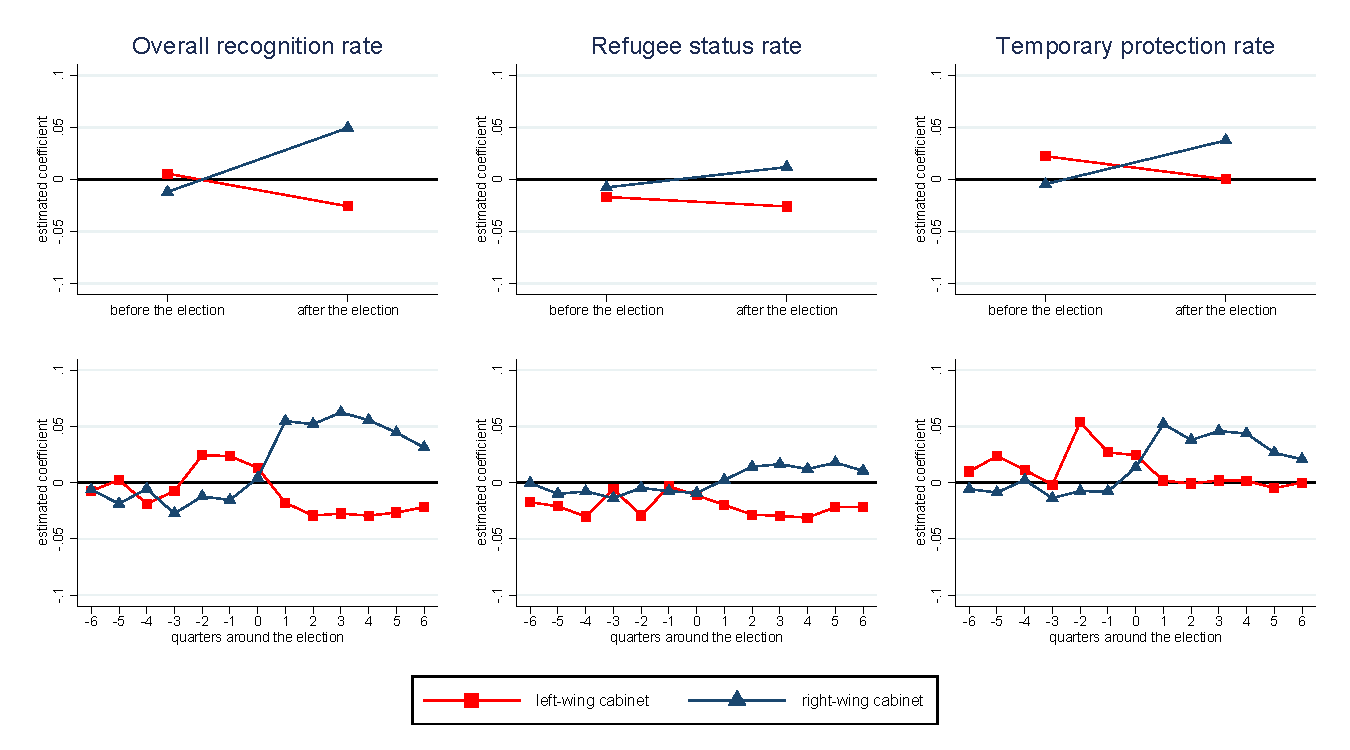
\includegraphics[width=\linewidth]{../results/decisions/dec_graphs_baseline.pdf}
%		{\scriptsize Note: These figures show the time evolution of the overall recognition rate, the refugee status rate and the temporary protection rate as estimated in fixed effects regression with a set of dummies for before and after the election or a set of dummies for different quarters before and after an election in a quarter t = 0. Significant coefficients are indicated by filled plot markers. Periods in which the two coefficients are significantly different from each other are indicated with a grey background. \par}
%	\end{minipage}
%\end{figure}
%
%\begin{table}[!ht]\centering \scriptsize
\def\sym#1{\ifmmode^{#1}\else\(^{#1}\)\fi}
\caption{Coefficients before after model decisions baseline}
\begin{tabular}{l*{9}{c}}
\hline\hline
                    &\multicolumn{3}{c}{(acceptance rate)}&\multicolumn{3}{c}{(refugee status rate)}&\multicolumn{3}{c}{(temporaray protection rate)}\\
                    &\multicolumn{1}{c}{left}&\multicolumn{1}{c}{right}&\multicolumn{1}{c}{diff}&\multicolumn{1}{c}{left}&\multicolumn{1}{c}{right}&\multicolumn{1}{c}{diff}&\multicolumn{1}{c}{left}&\multicolumn{1}{c}{right}&\multicolumn{1}{c}{diff}\\
\hline
before              &     0.00568         &     -0.0118         &      0.0175         &     -0.0168\sym{**} &    -0.00716         &    -0.00966         &      0.0225\sym{***}&    -0.00469         &      0.0272\sym{***}\\
                    &   (0.00771)         &   (0.00738)         &    (0.0114)         &   (0.00530)         &   (0.00564)         &   (0.00762)         &   (0.00483)         &   (0.00519)         &   (0.00801)         \\
[0.5em]
after               &     -0.0256\sym{***}&      0.0496\sym{***}&     -0.0752\sym{***}&     -0.0257\sym{***}&      0.0123\sym{**} &     -0.0380\sym{***}&   0.0000830         &      0.0373\sym{***}&     -0.0372\sym{***}\\
                    &   (0.00760)         &   (0.00904)         &    (0.0133)         &   (0.00534)         &   (0.00416)         &   (0.00775)         &   (0.00377)         &   (0.00823)         &   (0.00839)         \\
\hline
Observations        &       12921         &       12921         &       12921         &       12921         &       12921         &       12921         &       12921         &       12921         &       12921         \\
\hline\hline
\multicolumn{10}{l}{\footnotesize Standard errors in parentheses \sym{*} \(p<0.05\), \sym{**} \(p<0.01\), \sym{***} \(p<0.001\)}\\
\end{tabular}
\end{table}

%\begin{table}[htbp]\centering
\def\sym#1{\ifmmode^{#1}\else\(^{#1}\)\fi}
\caption{Coefficients quarterly model Decisions}
\begin{tabular}{l*{6}{c}}
\hline\hline
                    &\multicolumn{1}{c}{(1)}&\multicolumn{1}{c}{(2)}&\multicolumn{1}{c}{(3)}&\multicolumn{1}{c}{(4)}&\multicolumn{1}{c}{(5)}&\multicolumn{1}{c}{(6)}\\
                    &\multicolumn{1}{c}{left\_pos}&\multicolumn{1}{c}{right\_pos}&\multicolumn{1}{c}{left\_ref}&\multicolumn{1}{c}{right\_ref}&\multicolumn{1}{c}{left\_temp}&\multicolumn{1}{c}{right\_temp}\\
\hline
 6 quarters before the election&     0.00309         &     -0.0993\sym{***}&      -0.110\sym{**} &     -0.0108         &      0.0519         &      -0.135\sym{***}\\
                    &    (0.0319)         &    (0.0290)         &    (0.0391)         &    (0.0257)         &    (0.0336)         &    (0.0306)         \\
[1em]
 5 quarters before the election&      0.0681         &     -0.0678         &      -0.115\sym{**} &     -0.0134         &       0.146\sym{***}&     -0.0941\sym{**} \\
                    &    (0.0437)         &    (0.0369)         &    (0.0382)         &    (0.0358)         &    (0.0409)         &    (0.0288)         \\
[1em]
 4 quarters before the election&     -0.0393         &     -0.0384         &      -0.209\sym{***}&     -0.0624         &      0.0917\sym{*}  &    -0.00152         \\
                    &    (0.0533)         &    (0.0374)         &    (0.0439)         &    (0.0398)         &    (0.0432)         &    (0.0349)         \\
[1em]
 3 quarters before the election&      0.0531         &     -0.0583         &      -0.107\sym{**} &     -0.0289         &      0.0961\sym{*}  &     -0.0539         \\
                    &    (0.0428)         &    (0.0443)         &    (0.0369)         &    (0.0479)         &    (0.0403)         &    (0.0348)         \\
[1em]
 2 quarters before the election&       0.177\sym{***}&     -0.0252         &      -0.177\sym{***}&     -0.0218         &       0.269\sym{***}&      0.0147         \\
                    &    (0.0425)         &    (0.0466)         &    (0.0402)         &    (0.0386)         &    (0.0359)         &    (0.0459)         \\
[1em]
 1 quarters before the election&       0.158\sym{**} &      0.0238         &     -0.0584         &      0.0542         &       0.166\sym{***}&      0.0449         \\
                    &    (0.0529)         &    (0.0516)         &    (0.0390)         &    (0.0437)         &    (0.0407)         &    (0.0464)         \\
[1em]
Quarter of the election&      0.0460         &      0.0489         &      -0.106\sym{*}  &      0.0178         &      0.0803\sym{*}  &      0.0618         \\
                    &    (0.0450)         &    (0.0415)         &    (0.0414)         &    (0.0305)         &    (0.0327)         &    (0.0429)         \\
[1em]
 1 quarters after the election&    -0.00651         &       0.142\sym{**} &      -0.100\sym{**} &      0.0765\sym{*}  &      0.0516         &      0.0997\sym{*}  \\
                    &    (0.0428)         &    (0.0478)         &    (0.0387)         &    (0.0320)         &    (0.0338)         &    (0.0465)         \\
[1em]
 2 quarters after the election&     -0.0521         &       0.142\sym{**} &      -0.107\sym{**} &       0.111\sym{**} &      0.0644\sym{*}  &      0.0651         \\
                    &    (0.0374)         &    (0.0452)         &    (0.0394)         &    (0.0343)         &    (0.0316)         &    (0.0455)         \\
[1em]
 3 quarters after the election&     -0.0284         &       0.224\sym{***}&      -0.107\sym{**} &       0.128\sym{***}&      0.0953\sym{**} &       0.137\sym{**} \\
                    &    (0.0339)         &    (0.0330)         &    (0.0354)         &    (0.0295)         &    (0.0295)         &    (0.0432)         \\
[1em]
 4 quarters after the election&     -0.0467         &       0.194\sym{***}&      -0.120\sym{***}&      0.0852\sym{*}  &      0.0993\sym{***}&       0.114\sym{**} \\
                    &    (0.0348)         &    (0.0330)         &    (0.0352)         &    (0.0358)         &    (0.0297)         &    (0.0415)         \\
[1em]
 5 quarters after the election&  -0.0000619         &       0.170\sym{***}&     -0.0910\sym{**} &       0.109\sym{***}&      0.0936\sym{**} &       0.121\sym{**} \\
                    &    (0.0350)         &    (0.0399)         &    (0.0339)         &    (0.0330)         &    (0.0348)         &    (0.0414)         \\
[1em]
 6 quarters after the election&     -0.0324         &       0.100\sym{***}&      -0.131\sym{**} &      0.0943\sym{**} &       0.108\sym{***}&      0.0336         \\
                    &    (0.0418)         &    (0.0293)         &    (0.0441)         &    (0.0290)         &    (0.0310)         &    (0.0342)         \\
\hline
Observations        &       15938         &       15938         &       15938         &       15938         &       15938         &       15938         \\
\hline\hline
\multicolumn{7}{l}{\footnotesize Standard errors in parentheses}\\
\multicolumn{7}{l}{\footnotesize \sym{*} \(p<0.05\), \sym{**} \(p<0.01\), \sym{***} \(p<0.001\)}\\
\end{tabular}
\end{table}



 %=================================================================================================

\clearpage
\FloatBarrier
\subsection{Robustness checks for overall recognition rate}

\begin{table}[htbp]\centering
\def\sym#1{\ifmmode^{#1}\else\(^{#1}\)\fi}
\caption{Determinats of acceptance\_rate - R1 - R6}
\begin{tabular}{l*{6}{c}}
\hline\hline
                    &\multicolumn{1}{c}{(1)}&\multicolumn{1}{c}{(2)}&\multicolumn{1}{c}{(3)}&\multicolumn{1}{c}{(4)}&\multicolumn{1}{c}{(5)}&\multicolumn{1}{c}{(6)}\\
                    &\multicolumn{1}{c}{Acceptance rate}&\multicolumn{1}{c}{Acceptance rate}&\multicolumn{1}{c}{Acceptance rate}&\multicolumn{1}{c}{Acceptance rate}&\multicolumn{1}{c}{Acceptance rate}&\multicolumn{1}{c}{Acceptance rate}\\
\hline
Political Terror Scale&      0.0251\sym{*}  &                     &      0.0270\sym{*}  &      0.0269\sym{*}  &      0.0269\sym{*}  &      0.0267\sym{*}  \\
                    &    (0.0107)         &                     &    (0.0110)         &    (0.0110)         &    (0.0109)         &    (0.0111)         \\
[1em]
Civic Liberty (FHI) &      0.0373         &                     &      0.0348         &      0.0344         &      0.0345         &      0.0348         \\
                    &    (0.0224)         &                     &    (0.0227)         &    (0.0226)         &    (0.0227)         &    (0.0227)         \\
[1em]
Political Rights (FHI)&    -0.00807         &                     &    -0.00819         &    -0.00788         &    -0.00792         &    -0.00857         \\
                    &    (0.0186)         &                     &    (0.0198)         &    (0.0199)         &    (0.0199)         &    (0.0201)         \\
[1em]
Quarterly civil war battle death (000s)&      0.0532\sym{***}&                     &      0.0528\sym{***}&      0.0532\sym{***}&      0.0532\sym{***}&      0.0531\sym{***}\\
                    &   (0.00481)         &                     &   (0.00514)         &   (0.00503)         &   (0.00504)         &   (0.00511)         \\
[1em]
Log origin country real GDP per capita&     -0.0208         &                     &     -0.0230         &     -0.0228         &     -0.0227         &     -0.0243         \\
                    &    (0.0286)         &                     &    (0.0324)         &    (0.0322)         &    (0.0322)         &    (0.0321)         \\
[1em]
Log destination country quarterly real GDP per capita&       0.206\sym{*}  &       0.235\sym{**} &       0.249\sym{**} &       0.224\sym{*}  &       0.222\sym{*}  &       0.224\sym{**} \\
                    &    (0.0844)         &    (0.0728)         &    (0.0888)         &    (0.0862)         &    (0.0873)         &    (0.0790)         \\
[1em]
Quarterly unemployment rate at destination&    0.000227         &    0.000159         &   -0.000697         &    0.000492         &  -0.0000701         &   -0.000664         \\
                    &   (0.00132)         &   (0.00137)         &   (0.00114)         &   (0.00117)         &   (0.00117)         &   (0.00110)         \\
[1em]
Log migrant stock in 2000/1&    0.000920         &     0.00114         &                     &                     &                     &                     \\
                    &   (0.00238)         &   (0.00242)         &                     &                     &                     &                     \\
[1em]
Log distance from origin to destination&     -0.0118         &     -0.0166         &                     &                     &                     &                     \\
                    &    (0.0195)         &    (0.0191)         &                     &                     &                     &                     \\
[1em]
Log total average asylum applications per capita in previous 5 years&                     &                     &     -0.0306\sym{**} &                     &                     &                     \\
                    &                     &                     &    (0.0114)         &                     &                     &                     \\
[1em]
Asylum policy index overall&                     &                     &                     &                     &  -0.0000649         &                     \\
                    &                     &                     &                     &                     &   (0.00205)         &                     \\
[1em]
Policy on access    &                     &                     &                     &                     &                     &      0.0180\sym{**} \\
                    &                     &                     &                     &                     &                     &   (0.00575)         \\
[1em]
Policy on processing&                     &                     &                     &                     &                     &     -0.0248\sym{***}\\
                    &                     &                     &                     &                     &                     &   (0.00378)         \\
[1em]
Policy on welfare   &                     &                     &                     &                     &                     &      0.0141\sym{**} \\
                    &                     &                     &                     &                     &                     &   (0.00487)         \\
[1em]
Cabinet position left * Before the election&     0.00483         &     0.00239         &     0.00549         &      0.0256\sym{***}&     0.00569         &     0.00900         \\
                    &   (0.00798)         &   (0.00874)         &   (0.00777)         &   (0.00712)         &   (0.00772)         &   (0.00783)         \\
[1em]
Cabinet position left * After the election&     -0.0251\sym{**} &     -0.0245\sym{**} &     -0.0231\sym{**} &    -0.00606         &     -0.0256\sym{**} &     -0.0237\sym{**} \\
                    &   (0.00760)         &   (0.00773)         &   (0.00730)         &   (0.00674)         &   (0.00762)         &   (0.00720)         \\
[1em]
Cabinet position right * Before the election&     -0.0109         &     -0.0111         &     -0.0113         &     -0.0276\sym{**} &     -0.0119         &     -0.0120         \\
                    &   (0.00772)         &   (0.00767)         &   (0.00730)         &   (0.00840)         &   (0.00744)         &   (0.00725)         \\
[1em]
Cabinet position right * After the election&      0.0510\sym{***}&      0.0502\sym{***}&      0.0475\sym{***}&      0.0330\sym{***}&      0.0495\sym{***}&      0.0511\sym{***}\\
                    &   (0.00927)         &   (0.00914)         &   (0.00876)         &   (0.00737)         &   (0.00927)         &   (0.00920)         \\
\hline
Observations        &       12921         &       12921         &       12921         &       12921         &       12921         &       12921         \\
Adjusted \(R^{2}\)  &       0.141         &       0.054         &       0.136         &       0.136         &       0.134         &       0.141         \\
Mean acceptance\_rate&       0.159         &       0.159         &       0.159         &       0.159         &       0.159         &       0.159         \\
Fixed Effects       &           O         &       O x T         &       D x O         &       D x O         &       D x O         &       D x O         \\
Destination dummies &         Yes         &         Yes         &          No         &          No         &          No         &          No         \\
Quarter-Year dummies&         Yes         &          No         &         Yes         &         Yes         &         Yes         &         Yes         \\
\hline\hline
\multicolumn{7}{l}{\footnotesize Standard errors in parentheses}\\
\multicolumn{7}{l}{\footnotesize \sym{*} \(p<0.05\), \sym{**} \(p<0.01\), \sym{***} \(p<0.001\)}\\
\end{tabular}
\end{table}


\clearpage
\FloatBarrier
\begin{figure}[!ht]
	\caption{Overall recognition rate: predicted pattern - R1 to R6}
	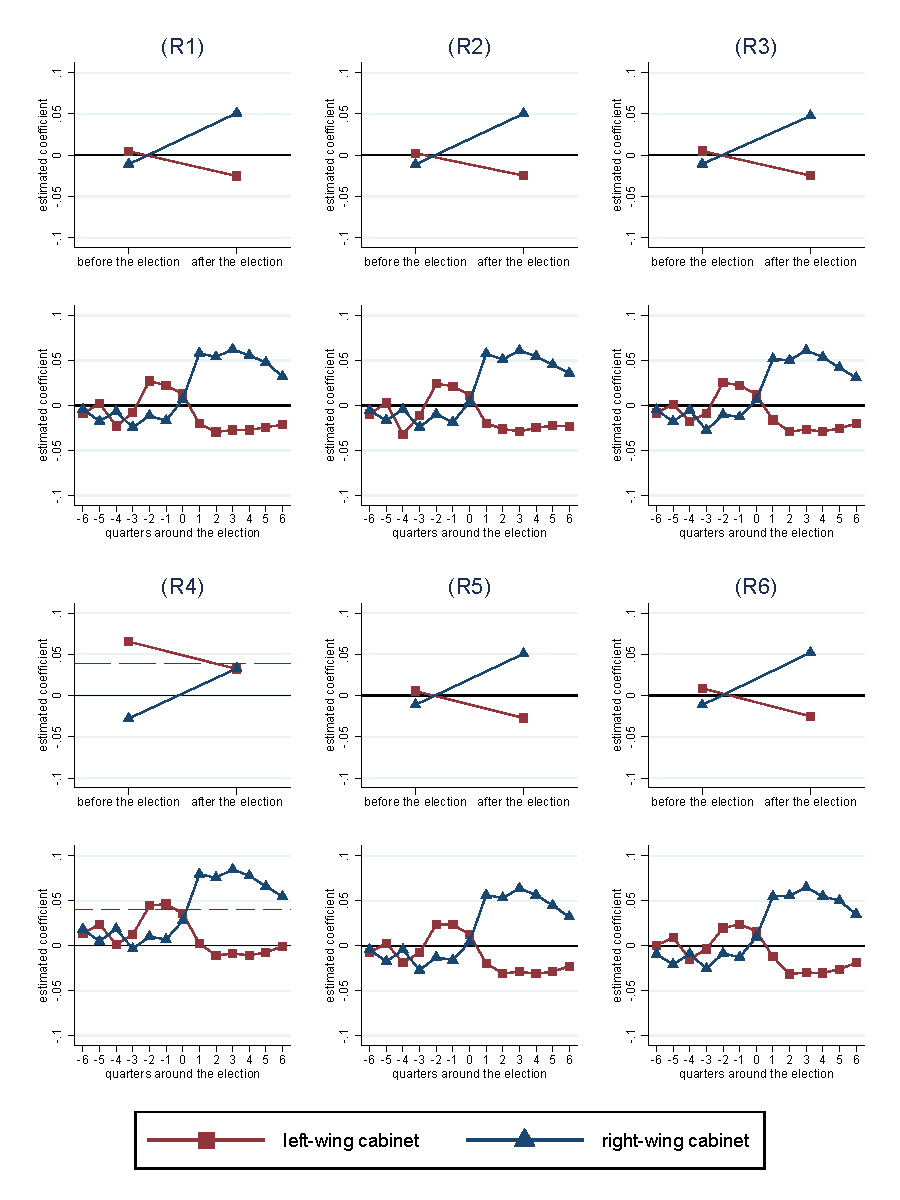
\includegraphics[width=1\textwidth]{../results/decisions/acceptance_rate_graphs_R1-R6.pdf}
	\scriptsize{Note: These figures show the time evolution of of the overall recognition rate as estimated in fixed effects regression with a set of dummies for before and after the election or a set of dummies for different quarters before and after an election in a quarter t = 0. Significant coefficients are indicated by filled plot markers. Periods in which the two coefficients are significantly different from each other are indicated with a grey background. The navy dashed line in sub-figure R4 shows the average overall recognition rate under right-wing cabinets in periods outside the election period. Significance of the coefficients of the right-wing cabinet in sub-figure R4 is reported for the distance to this average non-election period effect.}
\end{figure}

%\clearpage
%\FloatBarrier
%\begin{table}[htbp]\centering
\def\sym#1{\ifmmode^{#1}\else\(^{#1}\)\fi}
\caption{Coefficients before after model acceptance\_rate R1 - R2}
\begin{tabular}{l*{6}{c}}
\hline\hline
                    &\multicolumn{1}{c}{(1)}&\multicolumn{1}{c}{(2)}&\multicolumn{1}{c}{(3)}&\multicolumn{1}{c}{(4)}&\multicolumn{1}{c}{(5)}&\multicolumn{1}{c}{(6)}\\
                    &\multicolumn{1}{c}{left1\_R1}&\multicolumn{1}{c}{right1\_R1}&\multicolumn{1}{c}{diff1\_R1}&\multicolumn{1}{c}{left1\_R2}&\multicolumn{1}{c}{right1\_R2}&\multicolumn{1}{c}{diff1\_R2}\\
\hline
before              &     0.00487         &     -0.0109         &      0.0158         &     0.00245         &     -0.0111         &      0.0136         \\
                    &   (0.00797)         &   (0.00771)         &    (0.0120)         &   (0.00872)         &   (0.00766)         &    (0.0123)         \\
[1em]
after               &     -0.0252\sym{***}&      0.0511\sym{***}&     -0.0763\sym{***}&     -0.0247\sym{**} &      0.0503\sym{***}&     -0.0750\sym{***}\\
                    &   (0.00761)         &   (0.00925)         &    (0.0135)         &   (0.00773)         &   (0.00912)         &    (0.0136)         \\
\hline
Observations        &       12921         &       12921         &       12921         &       12921         &       12921         &       12921         \\
\hline\hline
\multicolumn{7}{l}{\footnotesize Standard errors in parentheses}\\
\multicolumn{7}{l}{\footnotesize \sym{*} \(p<0.05\), \sym{**} \(p<0.01\), \sym{***} \(p<0.001\)}\\
\end{tabular}
\end{table}

%\begin{table}[htbp]\centering
\def\sym#1{\ifmmode^{#1}\else\(^{#1}\)\fi}
\caption{Coefficients quarterly model acceptance\_rate R1 - R2}
\begin{tabular}{l*{6}{c}}
\hline\hline
                    &\multicolumn{1}{c}{(1)}&\multicolumn{1}{c}{(2)}&\multicolumn{1}{c}{(3)}&\multicolumn{1}{c}{(4)}&\multicolumn{1}{c}{(5)}&\multicolumn{1}{c}{(6)}\\
                    &\multicolumn{1}{c}{left2\_R1}&\multicolumn{1}{c}{right2\_R1}&\multicolumn{1}{c}{diff2\_R1}&\multicolumn{1}{c}{left2\_R2}&\multicolumn{1}{c}{right2\_R2}&\multicolumn{1}{c}{diff2\_R2}\\
\hline
 6 quarters before the election&    -0.00915         &    -0.00404         &    -0.00511         &    -0.00933         &    -0.00571         &    -0.00362         \\
                    &   (0.00959)         &    (0.0113)         &    (0.0168)         &    (0.0108)         &    (0.0114)         &    (0.0180)         \\
[1em]
 5 quarters before the election&     0.00248         &     -0.0175         &      0.0199         &     0.00268         &     -0.0165         &      0.0192         \\
                    &    (0.0139)         &   (0.00976)         &    (0.0163)         &    (0.0147)         &   (0.00958)         &    (0.0167)         \\
[1em]
 4 quarters before the election&     -0.0229         &    -0.00680         &     -0.0161         &     -0.0319\sym{*}  &    -0.00447         &     -0.0275         \\
                    &    (0.0140)         &    (0.0122)         &    (0.0185)         &    (0.0141)         &    (0.0113)         &    (0.0183)         \\
[1em]
 3 quarters before the election&    -0.00775         &     -0.0245\sym{*}  &      0.0167         &     -0.0112         &     -0.0241\sym{*}  &      0.0129         \\
                    &    (0.0124)         &    (0.0105)         &    (0.0163)         &    (0.0124)         &    (0.0101)         &    (0.0158)         \\
[1em]
 2 quarters before the election&      0.0272\sym{*}  &     -0.0114         &      0.0386\sym{*}  &      0.0243\sym{*}  &    -0.00969         &      0.0340\sym{*}  \\
                    &    (0.0113)         &    (0.0127)         &    (0.0159)         &    (0.0123)         &    (0.0124)         &    (0.0163)         \\
[1em]
 1 quarters before the election&      0.0225\sym{*}  &     -0.0171         &      0.0396\sym{*}  &      0.0215         &     -0.0185         &      0.0400\sym{*}  \\
                    &    (0.0112)         &    (0.0154)         &    (0.0198)         &    (0.0117)         &    (0.0153)         &    (0.0198)         \\
[1em]
Quarter of the election&      0.0127         &     0.00690         &     0.00584         &      0.0115         &     0.00381         &     0.00773         \\
                    &    (0.0115)         &    (0.0140)         &    (0.0171)         &    (0.0119)         &    (0.0149)         &    (0.0180)         \\
[1em]
 1 quarters after the election&     -0.0204\sym{*}  &      0.0580\sym{**} &     -0.0784\sym{***}&     -0.0200         &      0.0576\sym{**} &     -0.0776\sym{***}\\
                    &    (0.0103)         &    (0.0184)         &    (0.0227)         &    (0.0112)         &    (0.0179)         &    (0.0229)         \\
[1em]
 2 quarters after the election&     -0.0294\sym{**} &      0.0539\sym{**} &     -0.0834\sym{***}&     -0.0260\sym{*}  &      0.0511\sym{**} &     -0.0771\sym{***}\\
                    &    (0.0109)         &    (0.0170)         &    (0.0208)         &    (0.0111)         &    (0.0164)         &    (0.0211)         \\
[1em]
 3 quarters after the election&     -0.0273\sym{**} &      0.0625\sym{***}&     -0.0898\sym{***}&     -0.0289\sym{**} &      0.0611\sym{***}&     -0.0900\sym{***}\\
                    &   (0.00881)         &    (0.0133)         &    (0.0177)         &   (0.00886)         &    (0.0133)         &    (0.0180)         \\
[1em]
 4 quarters after the election&     -0.0273\sym{**} &      0.0557\sym{***}&     -0.0830\sym{***}&     -0.0249\sym{*}  &      0.0548\sym{***}&     -0.0797\sym{***}\\
                    &   (0.00991)         &   (0.00920)         &    (0.0152)         &    (0.0104)         &   (0.00964)         &    (0.0162)         \\
[1em]
 5 quarters after the election&     -0.0241\sym{*}  &      0.0479\sym{**} &     -0.0720\sym{***}&     -0.0222\sym{*}  &      0.0453\sym{**} &     -0.0675\sym{***}\\
                    &    (0.0105)         &    (0.0150)         &    (0.0206)         &    (0.0106)         &    (0.0151)         &    (0.0203)         \\
[1em]
 6 quarters after the election&     -0.0214         &      0.0323\sym{**} &     -0.0537\sym{**} &     -0.0231         &      0.0360\sym{***}&     -0.0591\sym{**} \\
                    &    (0.0134)         &    (0.0105)         &    (0.0197)         &    (0.0138)         &    (0.0102)         &    (0.0193)         \\
\hline
Observations        &       12921         &       12921         &       12921         &       12921         &       12921         &       12921         \\
\hline\hline
\multicolumn{7}{l}{\footnotesize Standard errors in parentheses}\\
\multicolumn{7}{l}{\footnotesize \sym{*} \(p<0.05\), \sym{**} \(p<0.01\), \sym{***} \(p<0.001\)}\\
\end{tabular}
\end{table}

%
%\clearpage
%\FloatBarrier
%\begin{table}[!ht]\centering \footnotesize
\def\sym#1{\ifmmode^{#1}\else\(^{#1}\)\fi}
\caption{Coefficients before after model acceptance\_rate R3 - R4}
\begin{tabular}{l*{6}{c}}
\hline\hline
                    &\multicolumn{1}{c}{(1)}&\multicolumn{1}{c}{(2)}&\multicolumn{1}{c}{(3)}&\multicolumn{1}{c}{(4)}&\multicolumn{1}{c}{(5)}&\multicolumn{1}{c}{(6)}\\
                    &\multicolumn{1}{c}{left1\_R3}&\multicolumn{1}{c}{right1\_R3}&\multicolumn{1}{c}{diff1\_R3}&\multicolumn{1}{c}{left1\_R4}&\multicolumn{1}{c}{right1\_R4}&\multicolumn{1}{c}{diff1\_R4}\\
\hline
before              &     0.00508         &     -0.0106         &      0.0157         &      0.0263\sym{***}&     -0.0279\sym{***}&      0.0150         \\
                    &   (0.00784)         &   (0.00734)         &    (0.0115)         &   (0.00717)         &   (0.00841)         &    (0.0117)         \\
[1em]
after               &     -0.0247\sym{***}&      0.0476\sym{***}&     -0.0723\sym{***}&    -0.00679         &      0.0327\sym{***}&     -0.0787\sym{***}\\
                    &   (0.00731)         &   (0.00885)         &    (0.0128)         &   (0.00672)         &   (0.00731)         &    (0.0138)         \\
\hline
Observations        &       12921         &       12921         &       12921         &       12921         &       12921         &       12921         \\
\hline\hline
\multicolumn{7}{l}{\footnotesize Standard errors in parentheses}\\
\multicolumn{7}{l}{\footnotesize \sym{*} \(p<0.05\), \sym{**} \(p<0.01\), \sym{***} \(p<0.001\)}\\
\end{tabular}
\end{table}

%\begin{table}[!ht]\centering \footnotesize
\def\sym#1{\ifmmode^{#1}\else\(^{#1}\)\fi}
\caption{Coefficients quarterly model acceptance\_rate R3 - R4}
\begin{tabular}{l*{6}{c}}
\hline\hline
                    &\multicolumn{1}{c}{(1)}&\multicolumn{1}{c}{(2)}&\multicolumn{1}{c}{(3)}&\multicolumn{1}{c}{(4)}&\multicolumn{1}{c}{(5)}&\multicolumn{1}{c}{(6)}\\
                    &\multicolumn{1}{c}{left2\_R3}&\multicolumn{1}{c}{right2\_R3}&\multicolumn{1}{c}{diff2\_R3}&\multicolumn{1}{c}{left2\_R4}&\multicolumn{1}{c}{right2\_R4}&\multicolumn{1}{c}{diff2\_R4}\\
\hline
 6 quarters before the election&    -0.00823         &    -0.00489         &    -0.00334         &      0.0141         &     -0.0215\sym{*}  &    -0.00456         \\
                    &   (0.00962)         &    (0.0117)         &    (0.0168)         &   (0.00947)         &   (0.00984)         &    (0.0170)         \\
[1em]
 5 quarters before the election&     0.00129         &     -0.0179         &      0.0192         &      0.0239         &     -0.0351\sym{***}&      0.0188         \\
                    &    (0.0132)         &   (0.00969)         &    (0.0153)         &    (0.0130)         &   (0.00962)         &    (0.0154)         \\
[1em]
 4 quarters before the election&     -0.0181         &    -0.00514         &     -0.0130         &     0.00144         &     -0.0215         &     -0.0173         \\
                    &    (0.0133)         &    (0.0114)         &    (0.0176)         &    (0.0122)         &    (0.0115)         &    (0.0180)         \\
[1em]
 3 quarters before the election&    -0.00867         &     -0.0276\sym{**} &      0.0189         &      0.0124         &     -0.0435\sym{***}&      0.0157         \\
                    &    (0.0123)         &    (0.0106)         &    (0.0157)         &    (0.0130)         &    (0.0123)         &    (0.0158)         \\
[1em]
 2 quarters before the election&      0.0252\sym{*}  &     -0.0102         &      0.0354\sym{*}  &      0.0446\sym{***}&     -0.0298\sym{*}  &      0.0342\sym{*}  \\
                    &    (0.0111)         &    (0.0121)         &    (0.0153)         &   (0.00975)         &    (0.0128)         &    (0.0158)         \\
[1em]
 1 quarters before the election&      0.0226\sym{*}  &     -0.0129         &      0.0354         &      0.0464\sym{***}&     -0.0329\sym{*}  &      0.0391\sym{*}  \\
                    &    (0.0108)         &    (0.0140)         &    (0.0186)         &    (0.0105)         &    (0.0153)         &    (0.0190)         \\
[1em]
Quarter of the election&      0.0120         &     0.00634         &     0.00564         &      0.0358\sym{**} &     -0.0123         &     0.00797         \\
                    &    (0.0117)         &    (0.0124)         &    (0.0161)         &    (0.0120)         &    (0.0155)         &    (0.0162)         \\
[1em]
 1 quarters after the election&     -0.0161         &      0.0517\sym{**} &     -0.0678\sym{**} &     0.00246         &      0.0395\sym{*}  &     -0.0773\sym{***}\\
                    &   (0.00998)         &    (0.0176)         &    (0.0210)         &   (0.00994)         &    (0.0169)         &    (0.0220)         \\
[1em]
 2 quarters after the election&     -0.0290\sym{**} &      0.0501\sym{**} &     -0.0791\sym{***}&     -0.0105         &      0.0357\sym{*}  &     -0.0864\sym{***}\\
                    &    (0.0105)         &    (0.0164)         &    (0.0203)         &    (0.0109)         &    (0.0148)         &    (0.0217)         \\
[1em]
 3 quarters after the election&     -0.0268\sym{**} &      0.0612\sym{***}&     -0.0880\sym{***}&    -0.00890         &      0.0448\sym{***}&     -0.0939\sym{***}\\
                    &   (0.00845)         &    (0.0128)         &    (0.0174)         &   (0.00839)         &    (0.0110)         &    (0.0181)         \\
[1em]
 4 quarters after the election&     -0.0289\sym{**} &      0.0536\sym{***}&     -0.0825\sym{***}&     -0.0104         &      0.0376\sym{***}&     -0.0882\sym{***}\\
                    &   (0.00985)         &   (0.00906)         &    (0.0150)         &   (0.00839)         &   (0.00946)         &    (0.0155)         \\
[1em]
 5 quarters after the election&     -0.0254\sym{*}  &      0.0418\sym{**} &     -0.0673\sym{***}&    -0.00734         &      0.0259\sym{*}  &     -0.0734\sym{***}\\
                    &    (0.0103)         &    (0.0144)         &    (0.0199)         &   (0.00979)         &    (0.0123)         &    (0.0206)         \\
[1em]
 6 quarters after the election&     -0.0203         &      0.0308\sym{**} &     -0.0511\sym{**} &   -0.000438         &      0.0148         &     -0.0554\sym{**} \\
                    &    (0.0130)         &    (0.0100)         &    (0.0184)         &    (0.0126)         &    (0.0100)         &    (0.0185)         \\
\hline
Observations        &       12921         &       12921         &       12921         &       12921         &       12921         &       12921         \\
\hline\hline
\multicolumn{7}{l}{\footnotesize Standard errors in parentheses}\\
\multicolumn{7}{l}{\footnotesize \sym{*} \(p<0.05\), \sym{**} \(p<0.01\), \sym{***} \(p<0.001\)}\\
\end{tabular}
\end{table}

%
%\clearpage
%\FloatBarrier
%\begin{table}[htbp]\centering
\def\sym#1{\ifmmode^{#1}\else\(^{#1}\)\fi}
\caption{Coefficients before after model acceptance\_rate R5 - R6}
\begin{tabular}{l*{6}{c}}
\hline\hline
                    &\multicolumn{1}{c}{(1)}&\multicolumn{1}{c}{(2)}&\multicolumn{1}{c}{(3)}&\multicolumn{1}{c}{(4)}&\multicolumn{1}{c}{(5)}&\multicolumn{1}{c}{(6)}\\
                    &\multicolumn{1}{c}{left1\_R5}&\multicolumn{1}{c}{right1\_R5}&\multicolumn{1}{c}{diff1\_R5}&\multicolumn{1}{c}{left1\_R6}&\multicolumn{1}{c}{right1\_R6}&\multicolumn{1}{c}{diff1\_R6}\\
\hline
before              &     0.00539         &     -0.0113         &      0.0167         &     0.00867         &     -0.0115         &      0.0202         \\
                    &   (0.00776)         &   (0.00749)         &    (0.0116)         &   (0.00786)         &   (0.00731)         &    (0.0115)         \\
[1em]
after               &     -0.0272\sym{***}&      0.0506\sym{***}&     -0.0778\sym{***}&     -0.0251\sym{***}&      0.0520\sym{***}&     -0.0771\sym{***}\\
                    &   (0.00756)         &   (0.00936)         &    (0.0135)         &   (0.00714)         &   (0.00928)         &    (0.0128)         \\
\hline
Observations        &       12921         &       12921         &       12921         &       12921         &       12921         &       12921         \\
\hline\hline
\multicolumn{7}{l}{\footnotesize Standard errors in parentheses}\\
\multicolumn{7}{l}{\footnotesize \sym{*} \(p<0.05\), \sym{**} \(p<0.01\), \sym{***} \(p<0.001\)}\\
\end{tabular}
\end{table}

%\begin{table}[!ht]\centering \footnotesize
\def\sym#1{\ifmmode^{#1}\else\(^{#1}\)\fi}
\caption{Coefficients quarterly model acceptance\_rate R5 - R6}
\begin{tabular}{l*{6}{c}}
\hline\hline
                    &\multicolumn{1}{c}{(1)}&\multicolumn{1}{c}{(2)}&\multicolumn{1}{c}{(3)}&\multicolumn{1}{c}{(4)}&\multicolumn{1}{c}{(5)}&\multicolumn{1}{c}{(6)}\\
                    &\multicolumn{1}{c}{left2\_R5}&\multicolumn{1}{c}{right2\_R5}&\multicolumn{1}{c}{diff2\_R5}&\multicolumn{1}{c}{left2\_R6}&\multicolumn{1}{c}{right2\_R6}&\multicolumn{1}{c}{diff2\_R6}\\
\hline
 6 quarters before the election&    -0.00736         &    -0.00419         &    -0.00317         &    0.000462         &    -0.00934         &     0.00980         \\
                    &   (0.00958)         &    (0.0118)         &    (0.0168)         &   (0.00988)         &    (0.0120)         &    (0.0174)         \\
[1em]
 5 quarters before the election&     0.00270         &     -0.0176         &      0.0203         &     0.00915         &     -0.0209\sym{*}  &      0.0301         \\
                    &    (0.0130)         &   (0.00968)         &    (0.0152)         &    (0.0137)         &   (0.00979)         &    (0.0163)         \\
[1em]
 4 quarters before the election&     -0.0189         &    -0.00451         &     -0.0144         &     -0.0149         &    -0.00894         &    -0.00596         \\
                    &    (0.0133)         &    (0.0115)         &    (0.0177)         &    (0.0132)         &    (0.0117)         &    (0.0177)         \\
[1em]
 3 quarters before the election&    -0.00781         &     -0.0273\sym{*}  &      0.0194         &    -0.00354         &     -0.0254\sym{*}  &      0.0218         \\
                    &    (0.0123)         &    (0.0106)         &    (0.0158)         &    (0.0122)         &    (0.0103)         &    (0.0160)         \\
[1em]
 2 quarters before the election&      0.0240\sym{*}  &     -0.0126         &      0.0366\sym{*}  &      0.0196         &    -0.00854         &      0.0281         \\
                    &    (0.0112)         &    (0.0123)         &    (0.0154)         &    (0.0110)         &    (0.0124)         &    (0.0155)         \\
[1em]
 1 quarters before the election&      0.0233\sym{*}  &     -0.0159         &      0.0392\sym{*}  &      0.0238\sym{*}  &     -0.0128         &      0.0366\sym{*}  \\
                    &    (0.0108)         &    (0.0143)         &    (0.0189)         &    (0.0107)         &    (0.0132)         &    (0.0175)         \\
[1em]
Quarter of the election&      0.0126         &     0.00414         &     0.00847         &      0.0162         &     0.00960         &     0.00659         \\
                    &    (0.0116)         &    (0.0129)         &    (0.0165)         &    (0.0117)         &    (0.0125)         &    (0.0158)         \\
[1em]
 1 quarters after the election&     -0.0195         &      0.0564\sym{**} &     -0.0759\sym{***}&     -0.0124         &      0.0549\sym{**} &     -0.0673\sym{**} \\
                    &    (0.0102)         &    (0.0181)         &    (0.0220)         &    (0.0101)         &    (0.0180)         &    (0.0217)         \\
[1em]
 2 quarters after the election&     -0.0308\sym{**} &      0.0532\sym{**} &     -0.0841\sym{***}&     -0.0315\sym{**} &      0.0557\sym{***}&     -0.0872\sym{***}\\
                    &    (0.0106)         &    (0.0169)         &    (0.0211)         &    (0.0101)         &    (0.0168)         &    (0.0208)         \\
[1em]
 3 quarters after the election&     -0.0290\sym{***}&      0.0638\sym{***}&     -0.0928\sym{***}&     -0.0298\sym{***}&      0.0648\sym{***}&     -0.0946\sym{***}\\
                    &   (0.00866)         &    (0.0131)         &    (0.0177)         &   (0.00836)         &    (0.0130)         &    (0.0172)         \\
[1em]
 4 quarters after the election&     -0.0310\sym{**} &      0.0563\sym{***}&     -0.0873\sym{***}&     -0.0303\sym{**} &      0.0549\sym{***}&     -0.0852\sym{***}\\
                    &    (0.0101)         &   (0.00955)         &    (0.0155)         &   (0.00987)         &   (0.00927)         &    (0.0146)         \\
[1em]
 5 quarters after the election&     -0.0288\sym{**} &      0.0449\sym{**} &     -0.0737\sym{***}&     -0.0261\sym{*}  &      0.0502\sym{***}&     -0.0764\sym{***}\\
                    &    (0.0106)         &    (0.0148)         &    (0.0206)         &    (0.0106)         &    (0.0149)         &    (0.0202)         \\
[1em]
 6 quarters after the election&     -0.0228         &      0.0321\sym{**} &     -0.0549\sym{**} &     -0.0190         &      0.0350\sym{***}&     -0.0539\sym{**} \\
                    &    (0.0131)         &   (0.00995)         &    (0.0182)         &    (0.0130)         &   (0.00984)         &    (0.0179)         \\
\hline
Observations        &       12921         &       12921         &       12921         &       12921         &       12921         &       12921         \\
\hline\hline
\multicolumn{7}{l}{\footnotesize Standard errors in parentheses}\\
\multicolumn{7}{l}{\footnotesize \sym{*} \(p<0.05\), \sym{**} \(p<0.01\), \sym{***} \(p<0.001\)}\\
\end{tabular}
\end{table}





\clearpage
\FloatBarrier
\begin{table}[!ht]\centering \scriptsize
	\def\sym#1{\ifmmode^{#1}\else\(^{#1}\)\fi}
	\caption{Determinants of overall recognition rate - R7 - R12}
	\begin{tabular}{l*{6}{c}}
		\hline\hline
		&\multicolumn{1}{c}{(1)}     &\multicolumn{1}{c}{(2)}       &\multicolumn{1}{c}{(3)}       &\multicolumn{1}{c}{(4)}    	&\multicolumn{1}{c}{(5)}  	&\multicolumn{1}{c}{(6)}   \\
		&\multicolumn{1}{c}{R7}&\multicolumn{1}{c}{R8}&\multicolumn{1}{c}{R9}&\multicolumn{1}{c}{R10}&\multicolumn{1}{c}{R11}&\multicolumn{1}{c}{R12}\\ 
\hline
Political Terror Scale&      0.0257\sym{*}  &                     &      0.0276\sym{***}&      0.0276\sym{*}  &      0.0276\sym{*}  &      0.0218\sym{*}  \\
                    &    (0.0111)         &                     &   (0.00798)         &    (0.0111)         &    (0.0111)         &    (0.0102)         \\
[0,5em]
Civic Liberty (FHI) &      0.0341         &                     &      0.0341\sym{**} &      0.0341         &      0.0341         &      0.0382         \\
                    &    (0.0220)         &                     &    (0.0130)         &    (0.0226)         &    (0.0226)         &    (0.0194)         \\
[0,5em]
Political Rights (FHI)&    -0.00849         &                     &    -0.00828         &    -0.00828         &    -0.00828         &    -0.00792         \\
                    &    (0.0198)         &                     &    (0.0102)         &    (0.0198)         &    (0.0198)         &    (0.0159)         \\
[0,5em]
Quarterly civil war &      0.0518\sym{***}&                     &      0.0533\sym{***}&      0.0533\sym{***}&      0.0533\sym{***}&      0.0465\sym{***}\\
battle death (000s)                    &   (0.00529)         &                     &   (0.00616)         &   (0.00505)         &   (0.00505)         &   (0.00461)         \\
[0,5em]
Log origin country real &     -0.0137         &                     &     -0.0155         &     -0.0155         &     -0.0155         &     -0.0157         \\
GDP per capita                    &    (0.0349)         &                     &    (0.0230)         &    (0.0338)         &    (0.0338)         &    (0.0337)         \\
[0,5em]
Log destination country quarterly &       0.181\sym{*}  &       0.179         &       0.221\sym{*}  &       0.221\sym{*}  &       0.221\sym{*}  &      0.0718         \\
real GDP per capita                    &    (0.0850)         &    (0.0894)         &     (0.100)         &    (0.0878)         &    (0.0878)         &    (0.0723)         \\
[0,5em]
Quarterly unemployment rate &    -0.00232         &    -0.00170         &  -0.0000391         &  -0.0000391         &  -0.0000391         &   -0.000589         \\
at destination                    &   (0.00141)         &   (0.00135)         &   (0.00168)         &   (0.00116)         &   (0.00116)         &   (0.00118)         \\
[0,5em]
Log total decisions per capita &     -0.0319\sym{**} &                     &                     &                     &                     &                     \\
 in previous year                   &    (0.0117)         &                     &                     &                     &                     &                     \\
[0,5em]
Log dyadic decisions at destination  &     0.00822         &                     &                     &                     &                     &                     \\
per capita in previous year                    &   (0.00656)         &                     &                     &                     &                     &                     \\
[0,5em]
Log total first-time applications &                     &     -0.0321\sym{*}  &                     &                     &                     &                     \\
in the previous 2 quarters                    &                     &    (0.0132)         &                     &                     &                     &                     \\
[0,5em]
Log dyadic first-time applications &                     &      0.0165         &                     &                     &                     &                     \\
in the previous 2 quarters                    &                     &    (0.0109)         &                     &                     &                     &                     \\
[0,5em]
Years after 2007    &                     &                     &                     &      0.0452         &                     &                     \\
                    &                     &                     &                     &    (0.0289)         &                     &                     \\
[0,5em]
Cabinet position left * &     0.00679         &     0.00531         &     0.00565         &     0.00565         &     0.00565         &   -0.000532         \\
Before the election                    &   (0.00766)         &   (0.00797)         &   (0.00795)         &   (0.00771)         &   (0.00771)         &   (0.00622)         \\
[0,5em]
Cabinet position left * &     -0.0237\sym{**} &     -0.0250\sym{**} &     -0.0257\sym{***}&     -0.0257\sym{**} &     -0.0257\sym{**} &     -0.0140\sym{*}  \\
After the election                    &   (0.00729)         &   (0.00763)         &   (0.00664)         &   (0.00761)         &   (0.00761)         &   (0.00650)         \\
[0,5em]
Cabinet position right * &     -0.0125         &     -0.0129         &     -0.0119         &     -0.0119         &     -0.0119         &    0.000456         \\
Before the election                    &   (0.00745)         &   (0.00752)         &   (0.00703)         &   (0.00737)         &   (0.00737)         &   (0.00652)         \\
[0,5em]
Cabinet position right * &      0.0485\sym{***}&      0.0477\sym{***}&      0.0495\sym{***}&      0.0495\sym{***}&      0.0495\sym{***}&      0.0427\sym{***}\\
After the election                    &   (0.00882)         &   (0.00918)         &   (0.00781)         &   (0.00903)         &   (0.00903)         &   (0.00747)         \\
\hline
Observations        &       12921         &       12868         &       12921         &       12921         &       12921         &       17193         \\
Adjusted \(R^{2}\)  &       0.136         &       0.084         &       0.134         &       0.134         &       0.134         &       0.099         \\
Mean acceptance\_rate&       0.159         &       0.159         &       0.159         &       0.159         &       0.159         &       0.170         \\
Fixed Effects       &       D x O         &       D x O         &       D x O         &       D x O         &       D x O         &       D x O         \\
Destination dummies &          No         &          No         &          No         &          No         &          No         &          No         \\
Quarter-Year dummies&         Yes         &         Yes         &         Yes         &         Yes         &         Yes         &         Yes         \\
\hline\hline
\multicolumn{7}{l}{ Standard errors in parentheses \sym{*} \(p<0.05\), \sym{**} \(p<0.01\), \sym{***} \(p<0.001\)}\\
\end{tabular}
\end{table}


\clearpage
\FloatBarrier
\begin{figure}[!ht]
	\caption{Accaptace rate: predicted pattern - R7 to R12}
	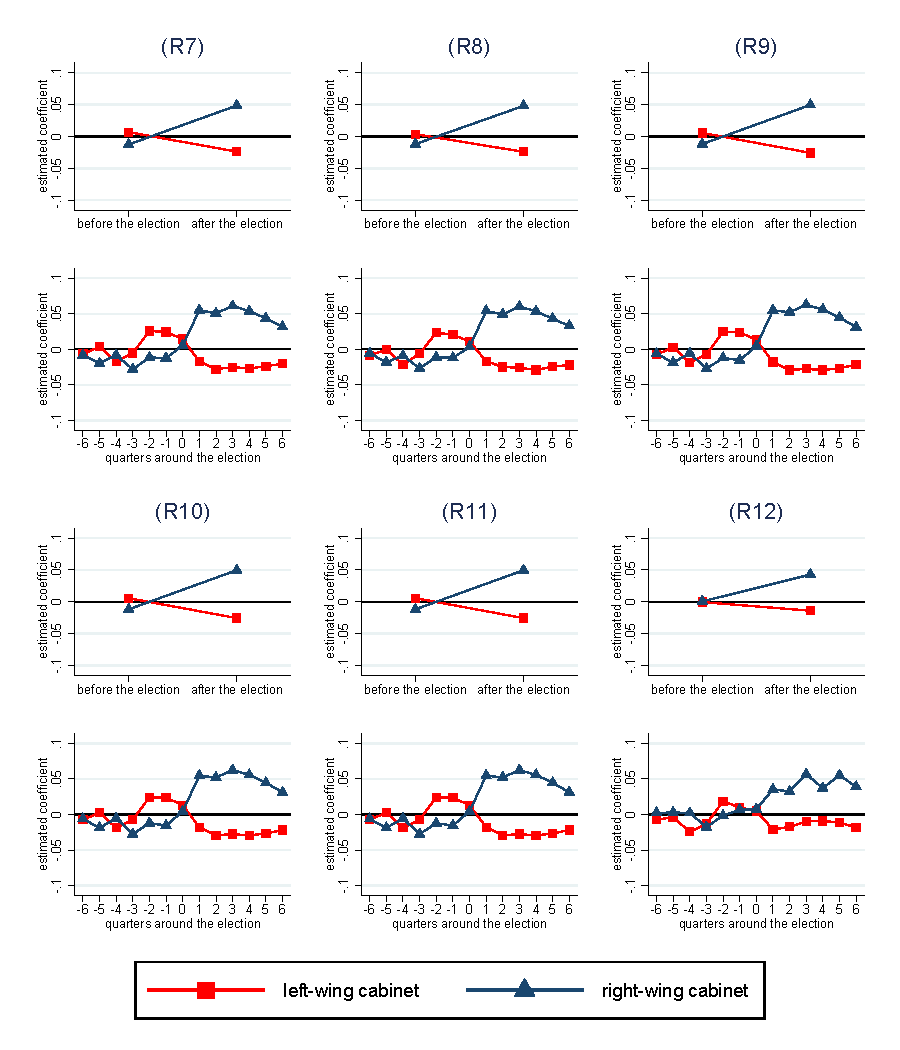
\includegraphics[width=1\textwidth]{../results/decisions/acceptance_rate_graphs_R7-R12.pdf}
	\scriptsize{Note: These figures show the time evolution of the overall recognition rate as estimated in fixed effects regression with a set of dummies for before and after the election or a set of dummies for different quarters before and after an election in a quarter t = 0. Significant coefficients are indicated by filled plot markers. Periods in which the two coefficients are significantly different from each other are indicated with a grey background.}
\end{figure}

%\clearpage
%\FloatBarrier
%\begin{table}[!ht]\centering \footnotesize
\def\sym#1{\ifmmode^{#1}\else\(^{#1}\)\fi}
\caption{Coefficients before after model acceptance rate R7 - R8}
\begin{tabular}{l*{6}{c}}
\hline\hline
                    &\multicolumn{3}{c}{(R7)}&\multicolumn{3}{c}{(R8)}\\
&\multicolumn{1}{c}{left}&\multicolumn{1}{c}{right}&\multicolumn{1}{c}{diff}&\multicolumn{1}{c}{left}&\multicolumn{1}{c}{right}&\multicolumn{1}{c}{diff}\\
\hline
before              &     0.00674         &     -0.0124         &      0.0191         &     0.00369         &     -0.0117         &      0.0154         \\
                    &   (0.00766)         &   (0.00745)         &    (0.0114)         &   (0.00775)         &   (0.00735)         &    (0.0114)         \\
[0,5em]
after               &     -0.0236\sym{**} &      0.0487\sym{***}&     -0.0723\sym{***}&     -0.0240\sym{**} &      0.0482\sym{***}&     -0.0722\sym{***}\\
                    &   (0.00727)         &   (0.00884)         &    (0.0126)         &   (0.00738)         &   (0.00888)         &    (0.0128)         \\
\hline
Observations        &       12921         &       12921         &       12921         &       12868         &       12868         &       12868         \\
\hline\hline
\multicolumn{7}{l}{\footnotesize Standard errors in parentheses \sym{*} \(p<0.05\), \sym{**} \(p<0.01\), \sym{***} \(p<0.001\)}\\
\end{tabular}
\end{table}

%\begin{table}[!ht]\centering \footnotesize
\def\sym#1{\ifmmode^{#1}\else\(^{#1}\)\fi}
\caption{Coefficients quarterly model acceptance rate R7 - R8}
\begin{tabular}{l*{6}{c}}
\hline\hline
                    &\multicolumn{3}{c}{(R7)}&\multicolumn{3}{c}{(R8)}\\
&\multicolumn{1}{c}{left}&\multicolumn{1}{c}{right}&\multicolumn{1}{c}{diff}&\multicolumn{1}{c}{left}&\multicolumn{1}{c}{right}&\multicolumn{1}{c}{diff}\\
\hline
 6 quarters before the election&    -0.00644         &    -0.00828         &     0.00184         &    -0.00837         &    -0.00561         &    -0.00276         \\
                    &   (0.00937)         &    (0.0113)         &    (0.0162)         &   (0.00951)         &    (0.0115)         &    (0.0166)         \\
[0,5em]
 5 quarters before the election&     0.00339         &     -0.0196\sym{*}  &      0.0230         &   -0.000552         &     -0.0180         &      0.0175         \\
                    &    (0.0131)         &   (0.00971)         &    (0.0154)         &    (0.0132)         &   (0.00968)         &    (0.0156)         \\
[0,5em]
 4 quarters before the election&     -0.0179         &    -0.00830         &    -0.00961         &     -0.0217         &    -0.00908         &     -0.0126         \\
                    &    (0.0133)         &    (0.0115)         &    (0.0174)         &    (0.0135)         &    (0.0114)         &    (0.0177)         \\
[0,5em]
 3 quarters before the election&    -0.00527         &     -0.0281\sym{**} &      0.0228         &    -0.00615         &     -0.0267\sym{*}  &      0.0205         \\
                    &    (0.0121)         &    (0.0107)         &    (0.0157)         &    (0.0121)         &    (0.0105)         &    (0.0156)         \\
[0,5em]
 2 quarters before the election&      0.0259\sym{*}  &     -0.0112         &      0.0371\sym{*}  &      0.0234\sym{*}  &     -0.0109         &      0.0344\sym{*}  \\
                    &    (0.0110)         &    (0.0124)         &    (0.0155)         &    (0.0111)         &    (0.0124)         &    (0.0154)         \\
[0,5em]
 1 quarters before the election&      0.0242\sym{*}  &     -0.0120         &      0.0362         &      0.0202         &     -0.0118         &      0.0320         \\
                    &    (0.0110)         &    (0.0143)         &    (0.0189)         &    (0.0108)         &    (0.0143)         &    (0.0189)         \\
[0,5em]
Quarter of the election&      0.0141         &     0.00518         &     0.00896         &      0.0111         &     0.00332         &     0.00773         \\
                    &    (0.0114)         &    (0.0127)         &    (0.0161)         &    (0.0113)         &    (0.0127)         &    (0.0159)         \\
[0,5em]
 1 quarters after the election&     -0.0170         &      0.0554\sym{**} &     -0.0723\sym{***}&     -0.0167         &      0.0541\sym{**} &     -0.0709\sym{***}\\
                    &   (0.00996)         &    (0.0178)         &    (0.0212)         &   (0.00998)         &    (0.0177)         &    (0.0210)         \\
[0,5em]
 2 quarters after the election&     -0.0279\sym{**} &      0.0509\sym{**} &     -0.0788\sym{***}&     -0.0248\sym{*}  &      0.0493\sym{**} &     -0.0741\sym{***}\\
                    &    (0.0106)         &    (0.0166)         &    (0.0206)         &    (0.0108)         &    (0.0165)         &    (0.0203)         \\
[0,5em]
 3 quarters after the election&     -0.0252\sym{**} &      0.0611\sym{***}&     -0.0863\sym{***}&     -0.0259\sym{**} &      0.0602\sym{***}&     -0.0861\sym{***}\\
                    &   (0.00833)         &    (0.0128)         &    (0.0172)         &   (0.00852)         &    (0.0127)         &    (0.0169)         \\
[0,5em]
 4 quarters after the election&     -0.0271\sym{**} &      0.0536\sym{***}&     -0.0807\sym{***}&     -0.0291\sym{**} &      0.0533\sym{***}&     -0.0824\sym{***}\\
                    &   (0.00990)         &   (0.00904)         &    (0.0147)         &   (0.00998)         &   (0.00912)         &    (0.0150)         \\
[0,5em]
 5 quarters after the election&     -0.0235\sym{*}  &      0.0437\sym{**} &     -0.0672\sym{***}&     -0.0243\sym{*}  &      0.0431\sym{**} &     -0.0674\sym{***}\\
                    &    (0.0104)         &    (0.0142)         &    (0.0195)         &    (0.0105)         &    (0.0144)         &    (0.0199)         \\
[0,5em]
 6 quarters after the election&     -0.0203         &      0.0317\sym{**} &     -0.0520\sym{**} &     -0.0220         &      0.0330\sym{**} &     -0.0550\sym{**} \\
                    &    (0.0127)         &   (0.00991)         &    (0.0180)         &    (0.0130)         &    (0.0104)         &    (0.0187)         \\
\hline
Observations        &       12921         &       12921         &       12921         &       12868         &       12868         &       12868         \\
\hline\hline
\multicolumn{7}{l}{\footnotesize Standard errors in parentheses \sym{*} \(p<0.05\), \sym{**} \(p<0.01\), \sym{***} \(p<0.001\)}\\
\end{tabular}
\end{table}

%
%\clearpage
%\FloatBarrier
%\begin{table}[!ht]\centering \footnotesize
\def\sym#1{\ifmmode^{#1}\else\(^{#1}\)\fi}
\caption{Coefficients before after model acceptance\_rate R9 - R10}
\begin{tabular}{l*{6}{c}}
\hline\hline
                    &\multicolumn{1}{c}{(1)}&\multicolumn{1}{c}{(2)}&\multicolumn{1}{c}{(3)}&\multicolumn{1}{c}{(4)}&\multicolumn{1}{c}{(5)}&\multicolumn{1}{c}{(6)}\\
                    &\multicolumn{1}{c}{left1\_R9}&\multicolumn{1}{c}{right1\_R9}&\multicolumn{1}{c}{diff1\_R9}&\multicolumn{1}{c}{left1\_R10}&\multicolumn{1}{c}{right1\_R10}&\multicolumn{1}{c}{diff1\_R10}\\
\hline
before              &     0.00565         &     -0.0119         &      0.0175         &     0.00565         &     -0.0119         &      0.0175         \\
                    &   (0.00795)         &   (0.00703)         &    (0.0108)         &   (0.00771)         &   (0.00737)         &    (0.0114)         \\
[1em]
after               &     -0.0257\sym{***}&      0.0495\sym{***}&     -0.0752\sym{***}&     -0.0257\sym{***}&      0.0495\sym{***}&     -0.0752\sym{***}\\
                    &   (0.00664)         &   (0.00781)         &   (0.00995)         &   (0.00761)         &   (0.00903)         &    (0.0133)         \\
\hline
Observations        &       12921         &       12921         &       12921         &       12921         &       12921         &       12921         \\
\hline\hline
\multicolumn{7}{l}{\footnotesize Standard errors in parentheses}\\
\multicolumn{7}{l}{\footnotesize \sym{*} \(p<0.05\), \sym{**} \(p<0.01\), \sym{***} \(p<0.001\)}\\
\end{tabular}
\end{table}

%\begin{table}[htbp]\centering
\def\sym#1{\ifmmode^{#1}\else\(^{#1}\)\fi}
\caption{Coefficients quarterly model acceptance\_rate R9 - R10}
\begin{tabular}{l*{6}{c}}
\hline\hline
                    &\multicolumn{1}{c}{(1)}&\multicolumn{1}{c}{(2)}&\multicolumn{1}{c}{(3)}&\multicolumn{1}{c}{(4)}&\multicolumn{1}{c}{(5)}&\multicolumn{1}{c}{(6)}\\
                    &\multicolumn{1}{c}{left2\_R9}&\multicolumn{1}{c}{right2\_R9}&\multicolumn{1}{c}{diff2\_R9}&\multicolumn{1}{c}{left2\_R10}&\multicolumn{1}{c}{right2\_R10}&\multicolumn{1}{c}{diff2\_R10}\\
\hline
 6 quarters before the election&    -0.00744         &    -0.00628         &    -0.00116         &    -0.00744         &    -0.00628         &    -0.00116         \\
                    &   (0.00968)         &    (0.0108)         &    (0.0151)         &   (0.00938)         &    (0.0115)         &    (0.0165)         \\
[1em]
 5 quarters before the election&     0.00254         &     -0.0187         &      0.0212         &     0.00254         &     -0.0187         &      0.0212         \\
                    &    (0.0112)         &    (0.0107)         &    (0.0160)         &    (0.0132)         &   (0.00963)         &    (0.0155)         \\
[1em]
 4 quarters before the election&     -0.0187         &    -0.00538         &     -0.0133         &     -0.0187         &    -0.00538         &     -0.0133         \\
                    &    (0.0128)         &    (0.0113)         &    (0.0167)         &    (0.0134)         &    (0.0113)         &    (0.0176)         \\
[1em]
 3 quarters before the election&    -0.00749         &     -0.0275\sym{**} &      0.0200         &    -0.00749         &     -0.0275\sym{**} &      0.0200         \\
                    &    (0.0141)         &    (0.0104)         &    (0.0168)         &    (0.0122)         &    (0.0106)         &    (0.0157)         \\
[1em]
 2 quarters before the election&      0.0245         &     -0.0122         &      0.0367         &      0.0245\sym{*}  &     -0.0122         &      0.0367\sym{*}  \\
                    &    (0.0142)         &    (0.0131)         &    (0.0192)         &    (0.0111)         &    (0.0125)         &    (0.0155)         \\
[1em]
 1 quarters before the election&      0.0237\sym{*}  &     -0.0155         &      0.0392\sym{*}  &      0.0237\sym{*}  &     -0.0155         &      0.0392\sym{*}  \\
                    &    (0.0120)         &    (0.0140)         &    (0.0181)         &    (0.0109)         &    (0.0145)         &    (0.0191)         \\
[1em]
Quarter of the election&      0.0132         &     0.00437         &     0.00887         &      0.0132         &     0.00437         &     0.00887         \\
                    &    (0.0111)         &    (0.0116)         &    (0.0148)         &    (0.0114)         &    (0.0129)         &    (0.0162)         \\
[1em]
 1 quarters after the election&     -0.0179         &      0.0548\sym{***}&     -0.0727\sym{***}&     -0.0179         &      0.0548\sym{**} &     -0.0727\sym{***}\\
                    &   (0.00973)         &    (0.0138)         &    (0.0165)         &    (0.0100)         &    (0.0178)         &    (0.0213)         \\
[1em]
 2 quarters after the election&     -0.0293\sym{**} &      0.0521\sym{***}&     -0.0814\sym{***}&     -0.0293\sym{**} &      0.0521\sym{**} &     -0.0814\sym{***}\\
                    &   (0.00996)         &    (0.0140)         &    (0.0164)         &    (0.0108)         &    (0.0168)         &    (0.0210)         \\
[1em]
 3 quarters after the election&     -0.0275\sym{**} &      0.0625\sym{***}&     -0.0900\sym{***}&     -0.0275\sym{**} &      0.0625\sym{***}&     -0.0900\sym{***}\\
                    &   (0.00914)         &    (0.0129)         &    (0.0155)         &   (0.00852)         &    (0.0130)         &    (0.0176)         \\
[1em]
 4 quarters after the election&     -0.0293\sym{**} &      0.0558\sym{***}&     -0.0851\sym{***}&     -0.0293\sym{**} &      0.0558\sym{***}&     -0.0851\sym{***}\\
                    &   (0.00896)         &    (0.0111)         &    (0.0145)         &    (0.0102)         &   (0.00923)         &    (0.0153)         \\
[1em]
 5 quarters after the election&     -0.0265\sym{**} &      0.0446\sym{***}&     -0.0711\sym{***}&     -0.0265\sym{*}  &      0.0446\sym{**} &     -0.0711\sym{***}\\
                    &   (0.00901)         &    (0.0120)         &    (0.0151)         &    (0.0107)         &    (0.0145)         &    (0.0204)         \\
[1em]
 6 quarters after the election&     -0.0218\sym{*}  &      0.0313\sym{**} &     -0.0530\sym{**} &     -0.0218         &      0.0313\sym{**} &     -0.0530\sym{**} \\
                    &    (0.0109)         &    (0.0120)         &    (0.0169)         &    (0.0129)         &    (0.0100)         &    (0.0184)         \\
\hline
Observations        &       12921         &       12921         &       12921         &       12921         &       12921         &       12921         \\
\hline\hline
\multicolumn{7}{l}{\footnotesize Standard errors in parentheses}\\
\multicolumn{7}{l}{\footnotesize \sym{*} \(p<0.05\), \sym{**} \(p<0.01\), \sym{***} \(p<0.001\)}\\
\end{tabular}
\end{table}

%
%\clearpage
%\FloatBarrier
%\begin{table}[htbp]\centering
\def\sym#1{\ifmmode^{#1}\else\(^{#1}\)\fi}
\caption{Coefficients before after model acceptance\_rate R11 - R12}
\begin{tabular}{l*{6}{c}}
\hline\hline
                    &\multicolumn{1}{c}{(1)}&\multicolumn{1}{c}{(2)}&\multicolumn{1}{c}{(3)}&\multicolumn{1}{c}{(4)}&\multicolumn{1}{c}{(5)}&\multicolumn{1}{c}{(6)}\\
                    &\multicolumn{1}{c}{left1\_R11}&\multicolumn{1}{c}{right1\_R11}&\multicolumn{1}{c}{diff1\_R11}&\multicolumn{1}{c}{left1\_R12}&\multicolumn{1}{c}{right1\_R12}&\multicolumn{1}{c}{diff1\_R12}\\
\hline
before              &     0.00568         &     -0.0118         &      0.0175         &   -0.000543         &    0.000499         &    -0.00104         \\
                    &   (0.00771)         &   (0.00738)         &    (0.0114)         &   (0.00623)         &   (0.00652)         &   (0.00937)         \\
[1em]
after               &     -0.0256\sym{***}&      0.0496\sym{***}&     -0.0752\sym{***}&     -0.0140\sym{*}  &      0.0427\sym{***}&     -0.0567\sym{***}\\
                    &   (0.00760)         &   (0.00904)         &    (0.0133)         &   (0.00648)         &   (0.00748)         &    (0.0112)         \\
\hline
Observations        &       12921         &       12921         &       12921         &       17193         &       17193         &       17193         \\
\hline\hline
\multicolumn{7}{l}{\footnotesize Standard errors in parentheses}\\
\multicolumn{7}{l}{\footnotesize \sym{*} \(p<0.05\), \sym{**} \(p<0.01\), \sym{***} \(p<0.001\)}\\
\end{tabular}
\end{table}

%\begin{table}[!ht]\centering \footnotesize
\def\sym#1{\ifmmode^{#1}\else\(^{#1}\)\fi}
\caption{Coefficients quarterly model acceptance\_rate R11 - R12}
\begin{tabular}{l*{6}{c}}
\hline\hline
                    &\multicolumn{1}{c}{(1)}&\multicolumn{1}{c}{(2)}&\multicolumn{1}{c}{(3)}&\multicolumn{1}{c}{(4)}&\multicolumn{1}{c}{(5)}&\multicolumn{1}{c}{(6)}\\
                    &\multicolumn{1}{c}{left2\_R10}&\multicolumn{1}{c}{right2\_R10}&\multicolumn{1}{c}{diff2\_R10}&\multicolumn{1}{c}{left2\_R12}&\multicolumn{1}{c}{right2\_R12}&\multicolumn{1}{c}{diff2\_R12}\\
\hline
 6 quarters before the election&    -0.00741         &    -0.00620         &    -0.00121         &    -0.00706         &     0.00227         &    -0.00933         \\
                    &   (0.00938)         &    (0.0115)         &    (0.0165)         &   (0.00958)         &   (0.00919)         &    (0.0139)         \\
[1em]
 5 quarters before the election&     0.00255         &     -0.0187         &      0.0213         &    -0.00392         &     0.00284         &    -0.00676         \\
                    &    (0.0132)         &   (0.00960)         &    (0.0155)         &    (0.0106)         &   (0.00919)         &    (0.0122)         \\
[1em]
 4 quarters before the election&     -0.0188         &    -0.00546         &     -0.0133         &     -0.0243\sym{*}  &     0.00221         &     -0.0265         \\
                    &    (0.0133)         &    (0.0113)         &    (0.0176)         &    (0.0110)         &    (0.0106)         &    (0.0154)         \\
[1em]
 3 quarters before the election&    -0.00746         &     -0.0275\sym{**} &      0.0200         &     -0.0133         &     -0.0176         &     0.00428         \\
                    &    (0.0123)         &    (0.0106)         &    (0.0157)         &    (0.0131)         &   (0.00930)         &    (0.0155)         \\
[1em]
 2 quarters before the election&      0.0244\sym{*}  &     -0.0122         &      0.0366\sym{*}  &      0.0186         &    -0.00164         &      0.0203         \\
                    &    (0.0111)         &    (0.0124)         &    (0.0155)         &   (0.00986)         &    (0.0109)         &    (0.0147)         \\
[1em]
 1 quarters before the election&      0.0236\sym{*}  &     -0.0155         &      0.0391\sym{*}  &      0.0100         &     0.00680         &     0.00321         \\
                    &    (0.0109)         &    (0.0144)         &    (0.0190)         &   (0.00884)         &    (0.0102)         &    (0.0113)         \\
[1em]
Quarter of the election&      0.0132         &     0.00431         &     0.00888         &     0.00504         &     0.00758         &    -0.00254         \\
                    &    (0.0114)         &    (0.0129)         &    (0.0162)         &   (0.00841)         &    (0.0116)         &    (0.0140)         \\
[1em]
 1 quarters after the election&     -0.0180         &      0.0548\sym{**} &     -0.0728\sym{***}&     -0.0211\sym{*}  &      0.0353\sym{**} &     -0.0564\sym{***}\\
                    &    (0.0100)         &    (0.0177)         &    (0.0212)         &   (0.00821)         &    (0.0128)         &    (0.0151)         \\
[1em]
 2 quarters after the election&     -0.0293\sym{**} &      0.0520\sym{**} &     -0.0813\sym{***}&     -0.0173\sym{*}  &      0.0324\sym{**} &     -0.0496\sym{***}\\
                    &    (0.0108)         &    (0.0167)         &    (0.0210)         &   (0.00851)         &    (0.0106)         &    (0.0140)         \\
[1em]
 3 quarters after the election&     -0.0275\sym{**} &      0.0625\sym{***}&     -0.0900\sym{***}&    -0.00980         &      0.0568\sym{***}&     -0.0666\sym{***}\\
                    &   (0.00855)         &    (0.0130)         &    (0.0177)         &   (0.00738)         &    (0.0119)         &    (0.0160)         \\
[1em]
 4 quarters after the election&     -0.0293\sym{**} &      0.0557\sym{***}&     -0.0850\sym{***}&    -0.00891         &      0.0371\sym{***}&     -0.0460\sym{***}\\
                    &    (0.0102)         &   (0.00922)         &    (0.0152)         &   (0.00965)         &   (0.00767)         &    (0.0130)         \\
[1em]
 5 quarters after the election&     -0.0265\sym{*}  &      0.0446\sym{**} &     -0.0711\sym{***}&     -0.0114         &      0.0552\sym{***}&     -0.0666\sym{***}\\
                    &    (0.0106)         &    (0.0145)         &    (0.0204)         &   (0.00920)         &    (0.0123)         &    (0.0175)         \\
[1em]
 6 quarters after the election&     -0.0218         &      0.0312\sym{**} &     -0.0530\sym{**} &     -0.0182         &      0.0390\sym{***}&     -0.0572\sym{***}\\
                    &    (0.0129)         &   (0.00999)         &    (0.0184)         &    (0.0106)         &   (0.00889)         &    (0.0138)         \\
\hline
Observations        &       12921         &       12921         &       12921         &       17193         &       17193         &       17193         \\
\hline\hline
\multicolumn{7}{l}{\footnotesize Standard errors in parentheses}\\
\multicolumn{7}{l}{\footnotesize \sym{*} \(p<0.05\), \sym{**} \(p<0.01\), \sym{***} \(p<0.001\)}\\
\end{tabular}
\end{table}



 %=========================================================================================

\clearpage
\FloatBarrier
\subsection{Robustness checks for refugee status rate}

\begin{table}[!ht]\centering \scriptsize
\def\sym#1{\ifmmode^{#1}\else\(^{#1}\)\fi}
\caption{Determinats of refugeestatus ate - R1 - R6}
\begin{tabular}{l*{6}{c}}
\hline\hline
	&\multicolumn{1}{c}{(1)}     &\multicolumn{1}{c}{(2)}       &\multicolumn{1}{c}{(3)}       &\multicolumn{1}{c}{(4)}    	&\multicolumn{1}{c}{(5)}  	&\multicolumn{1}{c}{(6)}   \\
                   &\multicolumn{1}{c}{R1}&\multicolumn{1}{c}{R2}&\multicolumn{1}{c}{R3}&\multicolumn{1}{c}{R4}&\multicolumn{1}{c}{R5}&\multicolumn{1}{c}{R6}\\
\hline
Political Terror Scale&      0.0276\sym{**} &                     &      0.0297\sym{**} &      0.0297\sym{**} &      0.0297\sym{**} &      0.0298\sym{**} \\
                    &   (0.00849)         &                     &   (0.00861)         &   (0.00864)         &   (0.00861)         &   (0.00861)         \\
[0,5em]
Civic Liberty (FHI) &      0.0247         &                     &      0.0219         &      0.0219         &      0.0218         &      0.0217         \\
                    &    (0.0139)         &                     &    (0.0145)         &    (0.0145)         &    (0.0145)         &    (0.0145)         \\
[0,5em]
Political Rights (FHI)&     -0.0105         &                     &    -0.00961         &    -0.00958         &    -0.00959         &    -0.00946         \\
                    &    (0.0108)         &                     &    (0.0116)         &    (0.0116)         &    (0.0116)         &    (0.0116)         \\
[0,5em]
Quarterly civil war &      0.0159\sym{***}&                     &      0.0160\sym{***}&      0.0160\sym{***}&      0.0160\sym{***}&      0.0160\sym{***}\\
battle death (000s)                    &   (0.00315)         &                     &   (0.00325)         &   (0.00322)         &   (0.00323)         &   (0.00323)         \\
[0,5em]
Log origin country &    -0.00769         &                     &     -0.0135         &     -0.0136         &     -0.0130         &     -0.0128         \\
real GDP per capita                    &    (0.0244)         &                     &    (0.0252)         &    (0.0252)         &    (0.0252)         &    (0.0253)         \\
[0,5em]
Log destination country &      -0.130\sym{*}  &      -0.112\sym{*}  &      -0.131\sym{*}  &      -0.130\sym{*}  &      -0.106         &      -0.113         \\
quarterly real GDP per capita                    &    (0.0602)         &    (0.0546)         &    (0.0578)         &    (0.0597)         &    (0.0605)         &    (0.0570)         \\
[0,5em]
Quarterly unemployment &    -0.00406\sym{*}  &    -0.00420\sym{*}  &    -0.00402\sym{*}  &    -0.00359\sym{*}  &    -0.00385\sym{*}  &    -0.00389\sym{*}  \\
rate at destination                    &   (0.00174)         &   (0.00181)         &   (0.00160)         &   (0.00158)         &   (0.00162)         &   (0.00165)         \\
[0,5em]
Log migrant stock in 2000/1&   -0.000204         &   -0.000114         &                     &                     &                     &                     \\
                    &   (0.00184)         &   (0.00186)         &                     &                     &                     &                     \\
[0,5em]
Log distance from origin to destination&      0.0101         &     0.00570         &                     &                     &                     &                     \\
                    &    (0.0160)         &    (0.0174)         &                     &                     &                     &                     \\
[0,5em]
Log total average asylum applications &                     &                     &  -0.0000712         &                     &                     &                     \\
per capita in previous 5 years                    &                     &                     &   (0.00778)         &                     &                     &                     \\
[0,5em]
Asylum policy index overall&                     &                     &                     &                     &     0.00257         &                     \\
                    &                     &                     &                     &                     &   (0.00153)         &                     \\
[0,5em]
Policy on access    &                     &                     &                     &                     &                     &   -0.000344         \\
                    &                     &                     &                     &                     &                     &   (0.00377)         \\
[0,5em]
Policy on processing&                     &                     &                     &                     &                     &     0.00865\sym{***}\\
                    &                     &                     &                     &                     &                     &   (0.00238)         \\
[0,5em]
Policy on welfare   &                     &                     &                     &                     &                     &    -0.00219         \\
                    &                     &                     &                     &                     &                     &   (0.00395)         \\
[0,5em]
Cabinet position left * &     -0.0174\sym{**} &     -0.0198\sym{**} &     -0.0168\sym{**} &    -0.00163         &     -0.0170\sym{**} &     -0.0177\sym{**} \\
Before the election                    &   (0.00556)         &   (0.00624)         &   (0.00531)         &   (0.00486)         &   (0.00532)         &   (0.00528)         \\
[0,5em]
Cabinet position left * &     -0.0263\sym{***}&     -0.0264\sym{***}&     -0.0257\sym{***}&     -0.0108\sym{*}  &     -0.0255\sym{***}&     -0.0257\sym{***}\\
After the election                    &   (0.00568)         &   (0.00584)         &   (0.00531)         &   (0.00512)         &   (0.00534)         &   (0.00521)         \\
[0,5em]
Cabinet position right * &    -0.00757         &    -0.00702         &    -0.00716         &     -0.0192\sym{**} &    -0.00660         &    -0.00647         \\
Before the election                    &   (0.00569)         &   (0.00570)         &   (0.00564)         &   (0.00638)         &   (0.00550)         &   (0.00550)         \\
[0,5em]
Cabinet position right *&      0.0123\sym{**} &      0.0124\sym{**} &      0.0123\sym{**} &   -0.000372         &      0.0143\sym{***}&      0.0136\sym{***}\\
 After the election                    &   (0.00405)         &   (0.00387)         &   (0.00406)         &   (0.00446)         &   (0.00392)         &   (0.00379)         \\
\hline
Observations        &       12921         &       12921         &       12921         &       12921         &       12921         &       12921         \\
Adjusted \(R^{2}\)  &       0.104         &       0.058         &       0.083         &       0.085         &       0.083         &       0.084         \\
Mean refugeestatus rate&      0.0866         &      0.0866         &      0.0866         &      0.0866         &      0.0866         &      0.0866         \\
Fixed Effects       &           O         &       O x T         &       D x O         &       D x O         &       D x O         &       D x O         \\
Destination dummies &         Yes         &         Yes         &          No         &          No         &          No         &          No         \\
Quarter-Year dummies&         Yes         &          No         &         Yes         &         Yes         &         Yes         &         Yes         \\
\hline\hline
\multicolumn{7}{l}{ Standard errors in parentheses \sym{*} \(p<0.05\), \sym{**} \(p<0.01\), \sym{***} \(p<0.001\)}\\
\end{tabular}
\end{table}


\clearpage
\FloatBarrier
\begin{figure}[!ht]
	\caption{Refugee status decisions per capita: predicted pattern - R1 to R6}
	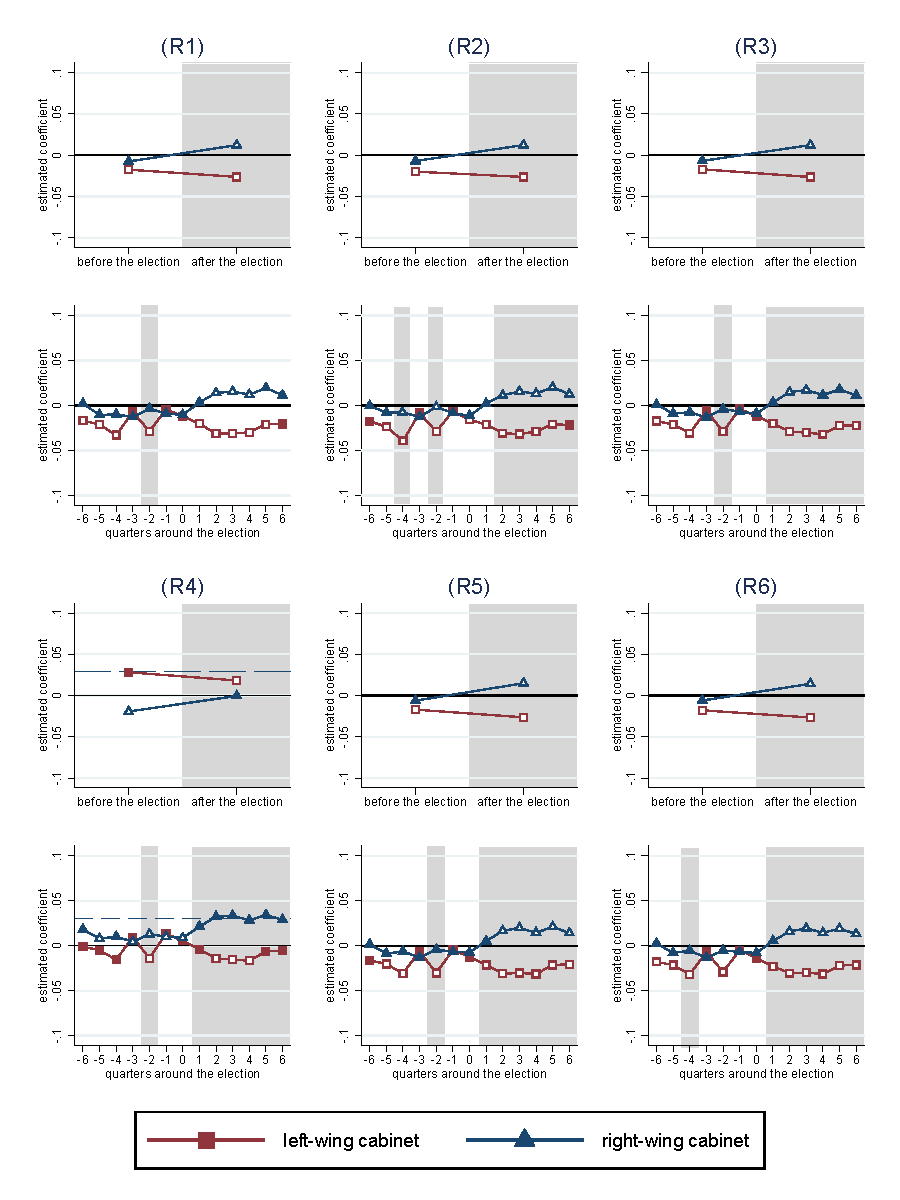
\includegraphics[width=1\textwidth]{../results/decisions/refugeestatus_rate_graphs_R1-R6.pdf}
	\scriptsize{Note: These figures show the time evolution of the refugee status rate as estimated in fixed effects regression with a set of dummies for before and after the election or a set of dummies for different quarters before and after an election in a quarter t = 0. Significant coefficients are indicated by filled plot markers. Periods in which the two coefficients are significantly different from each other are indicated with a grey background. The navy dashed line in sub-figure R4 shows the average refugee status rate under right-wing cabinets in periods outside the election period. Significance of the coefficients of the right-wing cabinet in sub-figure R4 is reported for the distance to this average non-election period effect.}
\end{figure}

%\clearpage
%\FloatBarrier
%\begin{table}[htbp]\centering
\def\sym#1{\ifmmode^{#1}\else\(^{#1}\)\fi}
\caption{Coefficients before after model refugeestatus\_rate R1 - R2}
\begin{tabular}{l*{6}{c}}
\hline\hline
                    &\multicolumn{1}{c}{(1)}&\multicolumn{1}{c}{(2)}&\multicolumn{1}{c}{(3)}&\multicolumn{1}{c}{(4)}&\multicolumn{1}{c}{(5)}&\multicolumn{1}{c}{(6)}\\
                    &\multicolumn{1}{c}{left1\_R1}&\multicolumn{1}{c}{right1\_R1}&\multicolumn{1}{c}{diff1\_R1}&\multicolumn{1}{c}{left1\_R2}&\multicolumn{1}{c}{right1\_R2}&\multicolumn{1}{c}{diff1\_R2}\\
\hline
before              &     -0.0175\sym{**} &    -0.00756         &    -0.00991         &     -0.0198\sym{**} &    -0.00700         &     -0.0128         \\
                    &   (0.00557)         &   (0.00570)         &   (0.00787)         &   (0.00624)         &   (0.00572)         &   (0.00818)         \\
[1em]
after               &     -0.0262\sym{***}&      0.0123\sym{**} &     -0.0385\sym{***}&     -0.0264\sym{***}&      0.0124\sym{**} &     -0.0387\sym{***}\\
                    &   (0.00566)         &   (0.00403)         &   (0.00787)         &   (0.00582)         &   (0.00387)         &   (0.00782)         \\
\hline
Observations        &       12921         &       12921         &       12921         &       12921         &       12921         &       12921         \\
\hline\hline
\multicolumn{7}{l}{\footnotesize Standard errors in parentheses}\\
\multicolumn{7}{l}{\footnotesize \sym{*} \(p<0.05\), \sym{**} \(p<0.01\), \sym{***} \(p<0.001\)}\\
\end{tabular}
\end{table}

%\begin{table}[!ht]\centering \footnotesize
\def\sym#1{\ifmmode^{#1}\else\(^{#1}\)\fi}
\caption{Coefficients quarterly model refugeestatus\_rate R1 - R2}
\begin{tabular}{l*{6}{c}}
\hline\hline
                    &\multicolumn{1}{c}{(1)}&\multicolumn{1}{c}{(2)}&\multicolumn{1}{c}{(3)}&\multicolumn{1}{c}{(4)}&\multicolumn{1}{c}{(5)}&\multicolumn{1}{c}{(6)}\\
                    &\multicolumn{1}{c}{left2\_R1}&\multicolumn{1}{c}{right2\_R1}&\multicolumn{1}{c}{diff2\_R1}&\multicolumn{1}{c}{left2\_R2}&\multicolumn{1}{c}{right2\_R2}&\multicolumn{1}{c}{diff2\_R2}\\
\hline
 6 quarters before the election&     -0.0167\sym{*}  &     0.00161         &     -0.0183         &     -0.0176         &   -0.000868         &     -0.0168         \\
                    &   (0.00806)         &   (0.00766)         &    (0.0123)         &   (0.00920)         &   (0.00788)         &    (0.0129)         \\
[1em]
 5 quarters before the election&     -0.0213\sym{*}  &     -0.0110         &     -0.0103         &     -0.0238\sym{**} &    -0.00850         &     -0.0153         \\
                    &   (0.00829)         &   (0.00863)         &    (0.0107)         &   (0.00903)         &   (0.00870)         &    (0.0109)         \\
[1em]
 4 quarters before the election&     -0.0322\sym{**} &    -0.00983         &     -0.0224         &     -0.0385\sym{***}&    -0.00762         &     -0.0309\sym{*}  \\
                    &    (0.0101)         &    (0.0111)         &    (0.0124)         &    (0.0105)         &    (0.0111)         &    (0.0128)         \\
[1em]
 3 quarters before the election&    -0.00749         &     -0.0130         &     0.00547         &    -0.00857         &     -0.0131         &     0.00450         \\
                    &    (0.0108)         &   (0.00728)         &    (0.0136)         &    (0.0112)         &   (0.00762)         &    (0.0139)         \\
[1em]
 2 quarters before the election&     -0.0288\sym{***}&    -0.00418         &     -0.0246         &     -0.0292\sym{***}&    -0.00249         &     -0.0267\sym{*}  \\
                    &   (0.00766)         &    (0.0101)         &    (0.0126)         &   (0.00815)         &    (0.0101)         &    (0.0128)         \\
[1em]
 1 quarters before the election&    -0.00405         &    -0.00980         &     0.00575         &    -0.00590         &    -0.00921         &     0.00331         \\
                    &   (0.00863)         &   (0.00930)         &    (0.0121)         &   (0.00876)         &   (0.00953)         &    (0.0118)         \\
[1em]
Quarter of the election&     -0.0115         &     -0.0103         &    -0.00115         &     -0.0156\sym{*}  &     -0.0115         &    -0.00410         \\
                    &   (0.00743)         &   (0.00755)         &    (0.0102)         &   (0.00792)         &   (0.00768)         &    (0.0105)         \\
[1em]
 1 quarters after the election&     -0.0206\sym{*}  &     0.00275         &     -0.0234         &     -0.0214\sym{*}  &     0.00142         &     -0.0228         \\
                    &   (0.00863)         &   (0.00863)         &    (0.0129)         &   (0.00982)         &   (0.00906)         &    (0.0147)         \\
[1em]
 2 quarters after the election&     -0.0314\sym{***}&      0.0134\sym{*}  &     -0.0449\sym{***}&     -0.0310\sym{***}&      0.0109         &     -0.0419\sym{***}\\
                    &   (0.00732)         &   (0.00661)         &   (0.00935)         &   (0.00752)         &   (0.00615)         &   (0.00934)         \\
[1em]
 3 quarters after the election&     -0.0311\sym{***}&      0.0153\sym{*}  &     -0.0464\sym{***}&     -0.0316\sym{***}&      0.0153\sym{*}  &     -0.0469\sym{***}\\
                    &   (0.00687)         &   (0.00669)         &   (0.00895)         &   (0.00699)         &   (0.00675)         &   (0.00923)         \\
[1em]
 4 quarters after the election&     -0.0297\sym{***}&      0.0123\sym{*}  &     -0.0420\sym{***}&     -0.0290\sym{***}&      0.0136\sym{*}  &     -0.0426\sym{***}\\
                    &   (0.00836)         &   (0.00579)         &    (0.0102)         &   (0.00854)         &   (0.00573)         &    (0.0103)         \\
[1em]
 5 quarters after the election&     -0.0215\sym{**} &      0.0192         &     -0.0407\sym{**} &     -0.0213\sym{**} &      0.0201         &     -0.0414\sym{**} \\
                    &   (0.00772)         &    (0.0103)         &    (0.0140)         &   (0.00755)         &    (0.0104)         &    (0.0139)         \\
[1em]
 6 quarters after the election&     -0.0208         &      0.0109         &     -0.0317\sym{*}  &     -0.0220\sym{*}  &      0.0120         &     -0.0340\sym{*}  \\
                    &    (0.0106)         &   (0.00732)         &    (0.0152)         &    (0.0112)         &   (0.00701)         &    (0.0153)         \\
\hline
Observations        &       12921         &       12921         &       12921         &       12921         &       12921         &       12921         \\
\hline\hline
\multicolumn{7}{l}{\footnotesize Standard errors in parentheses}\\
\multicolumn{7}{l}{\footnotesize \sym{*} \(p<0.05\), \sym{**} \(p<0.01\), \sym{***} \(p<0.001\)}\\
\end{tabular}
\end{table}

%
%\clearpage
%\FloatBarrier
%\begin{table}[htbp]\centering
\def\sym#1{\ifmmode^{#1}\else\(^{#1}\)\fi}
\caption{Coefficients before after model refugeestatus\_rate R3 - R4}
\begin{tabular}{l*{6}{c}}
\hline\hline
                    &\multicolumn{1}{c}{(1)}&\multicolumn{1}{c}{(2)}&\multicolumn{1}{c}{(3)}&\multicolumn{1}{c}{(4)}&\multicolumn{1}{c}{(5)}&\multicolumn{1}{c}{(6)}\\
                    &\multicolumn{1}{c}{left1\_R3}&\multicolumn{1}{c}{right1\_R3}&\multicolumn{1}{c}{diff1\_R3}&\multicolumn{1}{c}{left1\_R4}&\multicolumn{1}{c}{right1\_R4}&\multicolumn{1}{c}{diff1\_R4}\\
\hline
before              &     -0.0170\sym{**} &    -0.00687         &     -0.0101         &    -0.00125         &     -0.0193\sym{**} &     -0.0113         \\
                    &   (0.00532)         &   (0.00566)         &   (0.00765)         &   (0.00489)         &   (0.00643)         &   (0.00791)         \\
[1em]
after               &     -0.0264\sym{***}&      0.0123\sym{**} &     -0.0387\sym{***}&     -0.0112\sym{*}  &   -0.000508         &     -0.0401\sym{***}\\
                    &   (0.00540)         &   (0.00410)         &   (0.00773)         &   (0.00516)         &   (0.00443)         &   (0.00819)         \\
\hline
Observations        &       12921         &       12921         &       12921         &       12921         &       12921         &       12921         \\
\hline\hline
\multicolumn{7}{l}{\footnotesize Standard errors in parentheses}\\
\multicolumn{7}{l}{\footnotesize \sym{*} \(p<0.05\), \sym{**} \(p<0.01\), \sym{***} \(p<0.001\)}\\
\end{tabular}
\end{table}

%\begin{table}[!ht]\centering \footnotesize
\def\sym#1{\ifmmode^{#1}\else\(^{#1}\)\fi}
\caption{Coefficients quarterly model refugee status rate R3 - R4}
\begin{tabular}{l*{6}{c}}
\hline\hline
                    &\multicolumn{3}{c}{(R3)}&\multicolumn{3}{c}{(R4)}\\
&\multicolumn{1}{c}{left}&\multicolumn{1}{c}{right}&\multicolumn{1}{c}{diff}&\multicolumn{1}{c}{left}&\multicolumn{1}{c}{right}&\multicolumn{1}{c}{diff}\\
\hline
 6 quarters before the election&     -0.0174\sym{*}  &    0.000898         &     -0.0183         &    -0.00109         &     -0.0120         &     -0.0192         \\
                    &   (0.00841)         &   (0.00789)         &    (0.0127)         &   (0.00652)         &   (0.00764)         &    (0.0128)         \\
[0,5em]
 5 quarters before the election&     -0.0211\sym{*}  &    -0.00895         &     -0.0122         &    -0.00499         &     -0.0220\sym{*}  &     -0.0131         \\
                    &   (0.00825)         &   (0.00828)         &    (0.0103)         &   (0.00673)         &   (0.00965)         &    (0.0104)         \\
[0,5em]
 4 quarters before the election&     -0.0308\sym{**} &    -0.00750         &     -0.0233         &     -0.0155         &     -0.0200         &     -0.0256         \\
                    &   (0.00972)         &    (0.0111)         &    (0.0126)         &   (0.00842)         &    (0.0113)         &    (0.0131)         \\
[0,5em]
 3 quarters before the election&    -0.00561         &     -0.0134         &     0.00777         &     0.00952         &     -0.0255\sym{**} &     0.00492         \\
                    &   (0.00992)         &   (0.00713)         &    (0.0124)         &    (0.0108)         &   (0.00935)         &    (0.0124)         \\
[0,5em]
 2 quarters before the election&     -0.0291\sym{***}&    -0.00395         &     -0.0252\sym{*}  &     -0.0139\sym{*}  &     -0.0171\sym{*}  &     -0.0269\sym{*}  \\
                    &   (0.00755)         &   (0.00985)         &    (0.0126)         &   (0.00682)         &   (0.00815)         &    (0.0131)         \\
[0,5em]
 1 quarters before the election&    -0.00379         &    -0.00687         &     0.00307         &      0.0135         &     -0.0199\sym{*}  &     0.00329         \\
                    &   (0.00796)         &   (0.00927)         &    (0.0122)         &   (0.00834)         &   (0.00926)         &    (0.0119)         \\
[0,5em]
Quarter of the election&     -0.0118         &    -0.00913         &    -0.00267         &     0.00560         &     -0.0214\sym{*}  &    -0.00306         \\
                    &   (0.00726)         &   (0.00748)         &   (0.00974)         &   (0.00904)         &   (0.00914)         &   (0.00972)         \\
[0,5em]
 1 quarters after the election&     -0.0200\sym{*}  &     0.00345         &     -0.0235\sym{*}  &    -0.00397         &    -0.00869         &     -0.0254\sym{*}  \\
                    &   (0.00833)         &   (0.00791)         &    (0.0115)         &    (0.0105)         &   (0.00872)         &    (0.0116)         \\
[0,5em]
 2 quarters after the election&     -0.0288\sym{***}&      0.0149\sym{*}  &     -0.0437\sym{***}&     -0.0141\sym{*}  &     0.00212         &     -0.0463\sym{***}\\
                    &   (0.00723)         &   (0.00686)         &    (0.0102)         &   (0.00661)         &   (0.00747)         &    (0.0109)         \\
[0,5em]
 3 quarters after the election&     -0.0303\sym{***}&      0.0172\sym{*}  &     -0.0474\sym{***}&     -0.0154\sym{*}  &     0.00341         &     -0.0489\sym{***}\\
                    &   (0.00698)         &   (0.00703)         &   (0.00993)         &   (0.00662)         &   (0.00773)         &    (0.0101)         \\
[0,5em]
 4 quarters after the election&     -0.0320\sym{***}&      0.0117         &     -0.0436\sym{***}&     -0.0166\sym{**} &    -0.00178         &     -0.0449\sym{***}\\
                    &   (0.00831)         &   (0.00595)         &    (0.0101)         &   (0.00642)         &   (0.00793)         &    (0.0105)         \\
[0,5em]
 5 quarters after the election&     -0.0222\sym{**} &      0.0178         &     -0.0400\sym{**} &    -0.00632         &     0.00413         &     -0.0405\sym{**} \\
                    &   (0.00753)         &   (0.00981)         &    (0.0136)         &   (0.00801)         &   (0.00661)         &    (0.0139)         \\
[0,5em]
 6 quarters after the election&     -0.0220\sym{*}  &      0.0113         &     -0.0333\sym{*}  &    -0.00530         &    -0.00132         &     -0.0341\sym{*}  \\
                    &    (0.0101)         &   (0.00689)         &    (0.0147)         &   (0.00994)         &   (0.00745)         &    (0.0148)         \\
\hline
Observations        &       12921         &       12921         &       12921         &       12921         &       12921         &       12921         \\
\hline\hline
\multicolumn{7}{l}{\footnotesize Standard errors in parentheses \sym{*} \(p<0.05\), \sym{**} \(p<0.01\), \sym{***} \(p<0.001\)}\\
\end{tabular}
\end{table}

%
%\clearpage
%\FloatBarrier
%\begin{table}[htbp]\centering
\def\sym#1{\ifmmode^{#1}\else\(^{#1}\)\fi}
\caption{Coefficients before after model refugeestatus\_rate R5 - R6}
\begin{tabular}{l*{6}{c}}
\hline\hline
                    &\multicolumn{1}{c}{(1)}&\multicolumn{1}{c}{(2)}&\multicolumn{1}{c}{(3)}&\multicolumn{1}{c}{(4)}&\multicolumn{1}{c}{(5)}&\multicolumn{1}{c}{(6)}\\
                    &\multicolumn{1}{c}{left1\_R5}&\multicolumn{1}{c}{right1\_R5}&\multicolumn{1}{c}{diff1\_R5}&\multicolumn{1}{c}{left1\_R6}&\multicolumn{1}{c}{right1\_R6}&\multicolumn{1}{c}{diff1\_R6}\\
\hline
before              &     -0.0171\sym{**} &    -0.00626         &     -0.0109         &     -0.0179\sym{***}&    -0.00609         &     -0.0118         \\
                    &   (0.00532)         &   (0.00551)         &   (0.00750)         &   (0.00527)         &   (0.00551)         &   (0.00758)         \\
[1em]
after               &     -0.0264\sym{***}&      0.0149\sym{***}&     -0.0413\sym{***}&     -0.0267\sym{***}&      0.0142\sym{***}&     -0.0409\sym{***}\\
                    &   (0.00545)         &   (0.00396)         &   (0.00786)         &   (0.00532)         &   (0.00384)         &   (0.00752)         \\
\hline
Observations        &       12921         &       12921         &       12921         &       12921         &       12921         &       12921         \\
\hline\hline
\multicolumn{7}{l}{\footnotesize Standard errors in parentheses}\\
\multicolumn{7}{l}{\footnotesize \sym{*} \(p<0.05\), \sym{**} \(p<0.01\), \sym{***} \(p<0.001\)}\\
\end{tabular}
\end{table}

%\begin{table}[!ht]\centering \footnotesize
\def\sym#1{\ifmmode^{#1}\else\(^{#1}\)\fi}
\caption{Coefficients quarterly model refugee status rate R5 - R6}
\begin{tabular}{l*{6}{c}}
\hline\hline
                    &\multicolumn{3}{c}{(R5)}&\multicolumn{3}{c}{(R6)}\\
&\multicolumn{1}{c}{left}&\multicolumn{1}{c}{right}&\multicolumn{1}{c}{diff}&\multicolumn{1}{c}{left}&\multicolumn{1}{c}{right}&\multicolumn{1}{c}{diff}\\
\hline
 6 quarters before the election&     -0.0161         &     0.00156         &     -0.0177         &     -0.0178\sym{*}  &     0.00263         &     -0.0205         \\
                    &   (0.00847)         &   (0.00783)         &    (0.0128)         &   (0.00874)         &   (0.00795)         &    (0.0132)         \\
[0,5em]
 5 quarters before the election&     -0.0202\sym{*}  &    -0.00859         &     -0.0116         &     -0.0215\sym{**} &    -0.00794         &     -0.0136         \\
                    &   (0.00815)         &   (0.00816)         &    (0.0104)         &   (0.00800)         &   (0.00839)         &    (0.0107)         \\
[0,5em]
 4 quarters before the election&     -0.0308\sym{**} &    -0.00641         &     -0.0244         &     -0.0317\sym{**} &    -0.00549         &     -0.0262\sym{*}  \\
                    &   (0.00974)         &    (0.0109)         &    (0.0125)         &   (0.00967)         &    (0.0111)         &    (0.0126)         \\
[0,5em]
 3 quarters before the election&    -0.00614         &     -0.0131         &     0.00691         &    -0.00694         &     -0.0134         &     0.00649         \\
                    &    (0.0100)         &   (0.00709)         &    (0.0124)         &   (0.00993)         &   (0.00706)         &    (0.0125)         \\
[0,5em]
 2 quarters before the election&     -0.0302\sym{***}&    -0.00424         &     -0.0259\sym{*}  &     -0.0291\sym{***}&    -0.00533         &     -0.0237         \\
                    &   (0.00771)         &   (0.00981)         &    (0.0126)         &   (0.00777)         &   (0.00963)         &    (0.0123)         \\
[0,5em]
 1 quarters before the election&    -0.00479         &    -0.00671         &     0.00191         &    -0.00502         &    -0.00675         &     0.00174         \\
                    &   (0.00780)         &   (0.00910)         &    (0.0117)         &   (0.00775)         &   (0.00915)         &    (0.0115)         \\
[0,5em]
Quarter of the election&     -0.0124         &    -0.00752         &    -0.00484         &     -0.0136         &    -0.00801         &    -0.00556         \\
                    &   (0.00732)         &   (0.00736)         &   (0.00980)         &   (0.00734)         &   (0.00731)         &   (0.00989)         \\
[0,5em]
 1 quarters after the election&     -0.0213\sym{*}  &     0.00516         &     -0.0265\sym{*}  &     -0.0228\sym{**} &     0.00542         &     -0.0282\sym{*}  \\
                    &   (0.00845)         &   (0.00800)         &    (0.0118)         &   (0.00834)         &   (0.00801)         &    (0.0118)         \\
[0,5em]
 2 quarters after the election&     -0.0311\sym{***}&      0.0166\sym{*}  &     -0.0477\sym{***}&     -0.0305\sym{***}&      0.0159\sym{*}  &     -0.0464\sym{***}\\
                    &   (0.00713)         &   (0.00693)         &    (0.0100)         &   (0.00688)         &   (0.00694)         &   (0.00991)         \\
[0,5em]
 3 quarters after the election&     -0.0302\sym{***}&      0.0199\sym{**} &     -0.0501\sym{***}&     -0.0298\sym{***}&      0.0194\sym{**} &     -0.0492\sym{***}\\
                    &   (0.00696)         &   (0.00669)         &   (0.00949)         &   (0.00676)         &   (0.00660)         &   (0.00909)         \\
[0,5em]
 4 quarters after the election&     -0.0314\sym{***}&      0.0145\sym{*}  &     -0.0459\sym{***}&     -0.0315\sym{***}&      0.0144\sym{*}  &     -0.0459\sym{***}\\
                    &   (0.00833)         &   (0.00582)         &    (0.0104)         &   (0.00824)         &   (0.00584)         &   (0.00996)         \\
[0,5em]
 5 quarters after the election&     -0.0213\sym{**} &      0.0210\sym{*}  &     -0.0424\sym{**} &     -0.0220\sym{**} &      0.0191\sym{*}  &     -0.0411\sym{**} \\
                    &   (0.00762)         &   (0.00978)         &    (0.0139)         &   (0.00763)         &   (0.00933)         &    (0.0133)         \\
[0,5em]
 6 quarters after the election&     -0.0206\sym{*}  &      0.0142\sym{*}  &     -0.0349\sym{*}  &     -0.0213\sym{*}  &      0.0131         &     -0.0344\sym{*}  \\
                    &    (0.0103)         &   (0.00698)         &    (0.0147)         &    (0.0104)         &   (0.00703)         &    (0.0148)         \\
\hline
Observations        &       12921         &       12921         &       12921         &       12921         &       12921         &       12921         \\
\hline\hline
\multicolumn{7}{l}{\footnotesize Standard errors in parentheses \sym{*} \(p<0.05\), \sym{**} \(p<0.01\), \sym{***} \(p<0.001\)}\\
\end{tabular}
\end{table}




\clearpage
\FloatBarrier
\begin{table}[!ht]\centering \scriptsize
	\def\sym#1{\ifmmode^{#1}\else\(^{#1}\)\fi}
	\caption{Determinants of refugeestatus rate - R7 - R12}
	\begin{tabular}{l*{6}{c}}
		\hline\hline
		&\multicolumn{1}{c}{(1)}     &\multicolumn{1}{c}{(2)}       &\multicolumn{1}{c}{(3)}       &\multicolumn{1}{c}{(4)}    	&\multicolumn{1}{c}{(5)}  	&\multicolumn{1}{c}{(6)}   \\
		&\multicolumn{1}{c}{R7}&\multicolumn{1}{c}{R8}&\multicolumn{1}{c}{R9}&\multicolumn{1}{c}{R10}&\multicolumn{1}{c}{R11}&\multicolumn{1}{c}{R12}\\ 
\hline
Political Terror Scale&      0.0282\sym{**} &                     &      0.0302\sym{***}&      0.0302\sym{**} &      0.0302\sym{**} &      0.0238\sym{**} \\
                    &   (0.00811)         &                     &   (0.00625)         &   (0.00870)         &   (0.00870)         &   (0.00804)         \\
[0,5em]
Civic Liberty (FHI) &      0.0215         &                     &      0.0217\sym{*}  &      0.0217         &      0.0217         &      0.0209         \\
                    &    (0.0138)         &                     &    (0.0104)         &    (0.0144)         &    (0.0144)         &    (0.0119)         \\
[0,5em]
Political Rights (FHI)&     -0.0101         &                     &    -0.00989         &    -0.00989         &    -0.00989         &    -0.00671         \\
                    &    (0.0114)         &                     &   (0.00780)         &    (0.0115)         &    (0.0115)         &   (0.00870)         \\
[0,5em]
Quarterly civil war &      0.0148\sym{***}&                     &      0.0161         &      0.0161\sym{***}&      0.0161\sym{***}&      0.0150\sym{***}\\
battle death (000s)                    &   (0.00344)         &                     &   (0.00839)         &   (0.00326)         &   (0.00326)         &   (0.00344)         \\
[0,5em]
Log origin country real &    -0.00558         &                     &    -0.00751         &    -0.00751         &    -0.00751         &     -0.0115         \\
GDP per capita                    &    (0.0261)         &                     &    (0.0205)         &    (0.0258)         &    (0.0258)         &    (0.0246)         \\
[0,5em]
Log destination country quarterly &      -0.177\sym{**} &      -0.160\sym{*}  &      -0.148\sym{*}  &      -0.148\sym{*}  &      -0.148\sym{*}  &      -0.180\sym{**} \\
real GDP per capita                    &    (0.0646)         &    (0.0674)         &    (0.0701)         &    (0.0621)         &    (0.0621)         &    (0.0572)         \\
[0,5em]
Quarterly unemployment rate &    -0.00592\sym{**} &    -0.00485\sym{**} &    -0.00428\sym{**} &    -0.00428\sym{*}  &    -0.00428\sym{*}  &    -0.00349\sym{**} \\
at destination                    &   (0.00188)         &   (0.00181)         &   (0.00131)         &   (0.00167)         &   (0.00167)         &   (0.00119)         \\
[0,5em]
Log total decisions per capita &     -0.0237\sym{**} &                     &                     &                     &                     &                     \\
in previous year                    &   (0.00704)         &                     &                     &                     &                     &                     \\
[0,5em]
Log dyadic decisions at destination &     0.00809         &                     &                     &                     &                     &                     \\
per capita in previous year                    &   (0.00464)         &                     &                     &                     &                     &                     \\
[0,5em]
Log total first-time applications &                     &     -0.0159\sym{*}  &                     &                     &                     &                     \\
in the previous 2 quarters                    &                     &   (0.00658)         &                     &                     &                     &                     \\
[0,5em]
Log dyadic first-time applications &                     &      0.0134\sym{**} &                     &                     &                     &                     \\
in the previous 2 quarters                    &                     &   (0.00498)         &                     &                     &                     &                     \\
[0,5em]
Years after 2007    &                     &                     &                     &      0.0812\sym{**} &                     &                     \\
                    &                     &                     &                     &    (0.0273)         &                     &                     \\
[0,5em]
Cabinet position left * &     -0.0159\sym{**} &     -0.0167\sym{**} &     -0.0167\sym{**} &     -0.0167\sym{**} &     -0.0167\sym{**} &     -0.0165\sym{***}\\
Before the election                    &   (0.00527)         &   (0.00539)         &   (0.00553)         &   (0.00529)         &   (0.00529)         &   (0.00440)         \\
[0,5em]
Cabinet position left * &     -0.0247\sym{***}&     -0.0265\sym{***}&     -0.0259\sym{***}&     -0.0259\sym{***}&     -0.0259\sym{***}&     -0.0166\sym{**} \\
After the election                    &   (0.00524)         &   (0.00567)         &   (0.00542)         &   (0.00538)         &   (0.00538)         &   (0.00479)         \\
[0,5em]
Cabinet position right * &    -0.00786         &    -0.00804         &    -0.00752         &    -0.00752         &    -0.00752         &      0.0125\sym{**} \\
Before the election                    &   (0.00574)         &   (0.00572)         &   (0.00515)         &   (0.00563)         &   (0.00563)         &   (0.00457)         \\
[0,5em]
Cabinet position right * &      0.0114\sym{**} &      0.0117\sym{**} &      0.0120\sym{*}  &      0.0120\sym{**} &      0.0120\sym{**} &      0.0188\sym{***}\\
After the election                    &   (0.00419)         &   (0.00424)         &   (0.00538)         &   (0.00414)         &   (0.00414)         &   (0.00366)         \\
\hline
Observations        &       12921         &       12868         &       12921         &       12921         &       12921         &       17191         \\
Adjusted \(R^{2}\)  &       0.086         &       0.068         &       0.083         &       0.083         &       0.083         &       0.057         \\
Mean refugeestatus\_rate&      0.0866         &      0.0867         &      0.0866         &      0.0866         &      0.0866         &      0.0924         \\
Fixed Effects       &       D x O         &       D x O         &       D x O         &       D x O         &       D x O         &       D x O         \\
Destination dummies &          No         &          No         &          No         &          No         &          No         &          No         \\
Quarter-Year dummies&         Yes         &         Yes         &         Yes         &         Yes         &         Yes         &         Yes         \\
\hline\hline
\multicolumn{7}{l}{ Standard errors in parentheses \sym{*} \(p<0.05\), \sym{**} \(p<0.01\), \sym{***} \(p<0.001\)}\\
\end{tabular}
\end{table}


\clearpage
\FloatBarrier
\begin{figure}[!ht]
	\caption{Refugee status decisions per capita: predicted pattern - R7 to R12}
	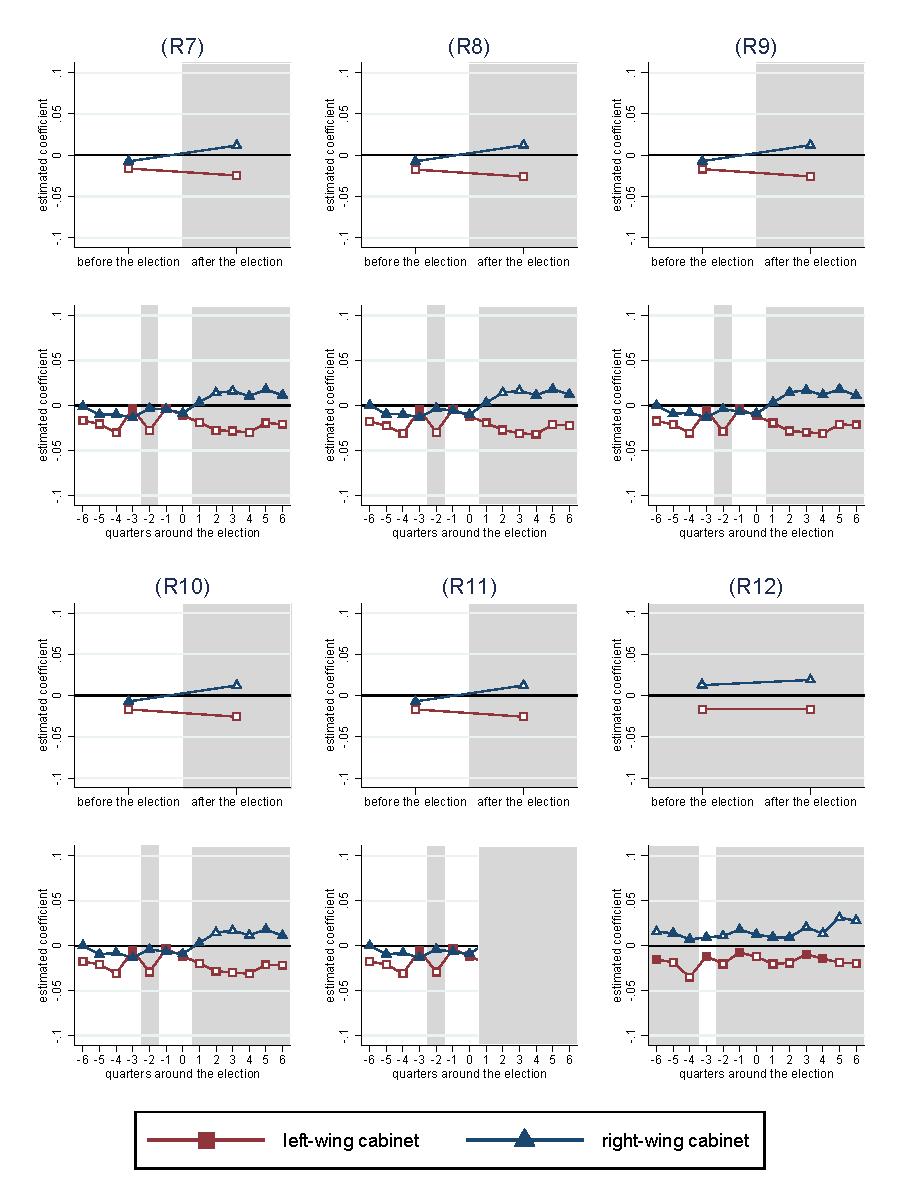
\includegraphics[width=1\textwidth]{../results/decisions/refugeestatus_rate_graphs_R7-R12.pdf}
	\scriptsize{Note: These figures show the time evolution of the refugee status rate as estimated in fixed effects regression with a set of dummies for before and after the election or a set of dummies for different quarters before and after an election in a quarter t = 0. Significant coefficients are indicated by filled plot markers. Periods in which the two coefficients are significantly different from each other are indicated with a grey background.}
\end{figure}

%\clearpage
%\FloatBarrier
%\begin{table}[htbp]\centering
\def\sym#1{\ifmmode^{#1}\else\(^{#1}\)\fi}
\caption{Coefficients before after model refugeestatus\_rate R7 - R8}
\begin{tabular}{l*{6}{c}}
\hline\hline
                    &\multicolumn{1}{c}{(1)}&\multicolumn{1}{c}{(2)}&\multicolumn{1}{c}{(3)}&\multicolumn{1}{c}{(4)}&\multicolumn{1}{c}{(5)}&\multicolumn{1}{c}{(6)}\\
                    &\multicolumn{1}{c}{left1\_R7}&\multicolumn{1}{c}{right1\_R7}&\multicolumn{1}{c}{diff1\_R7}&\multicolumn{1}{c}{left1\_R8}&\multicolumn{1}{c}{right1\_R8}&\multicolumn{1}{c}{diff1\_R8}\\
\hline
before              &     -0.0161\sym{**} &    -0.00737         &    -0.00870         &     -0.0174\sym{**} &    -0.00738         &     -0.0100         \\
                    &   (0.00530)         &   (0.00572)         &   (0.00775)         &   (0.00531)         &   (0.00564)         &   (0.00757)         \\
[1em]
after               &     -0.0246\sym{***}&      0.0118\sym{**} &     -0.0364\sym{***}&     -0.0260\sym{***}&      0.0122\sym{**} &     -0.0382\sym{***}\\
                    &   (0.00520)         &   (0.00420)         &   (0.00761)         &   (0.00545)         &   (0.00418)         &   (0.00789)         \\
\hline
Observations        &       12921         &       12921         &       12921         &       12868         &       12868         &       12868         \\
\hline\hline
\multicolumn{7}{l}{\footnotesize Standard errors in parentheses}\\
\multicolumn{7}{l}{\footnotesize \sym{*} \(p<0.05\), \sym{**} \(p<0.01\), \sym{***} \(p<0.001\)}\\
\end{tabular}
\end{table}

%\begin{table}[!ht]\centering \footnotesize
\def\sym#1{\ifmmode^{#1}\else\(^{#1}\)\fi}
\caption{Coefficients quarterly model refugeestatus\_rate R7 - R8}
\begin{tabular}{l*{6}{c}}
\hline\hline
                    &\multicolumn{1}{c}{(1)}&\multicolumn{1}{c}{(2)}&\multicolumn{1}{c}{(3)}&\multicolumn{1}{c}{(4)}&\multicolumn{1}{c}{(5)}&\multicolumn{1}{c}{(6)}\\
                    &\multicolumn{1}{c}{left2\_R7}&\multicolumn{1}{c}{right2\_R7}&\multicolumn{1}{c}{diff2\_R7}&\multicolumn{1}{c}{left2\_R8}&\multicolumn{1}{c}{right2\_R8}&\multicolumn{1}{c}{diff2\_R8}\\
\hline
 6 quarters before the election&     -0.0167\sym{*}  &    -0.00186         &     -0.0149         &     -0.0179\sym{*}  &   -0.000343         &     -0.0175         \\
                    &   (0.00833)         &   (0.00799)         &    (0.0126)         &   (0.00833)         &   (0.00792)         &    (0.0126)         \\
[1em]
 5 quarters before the election&     -0.0205\sym{*}  &     -0.0106         &    -0.00986         &     -0.0227\sym{**} &     -0.0100         &     -0.0127         \\
                    &   (0.00809)         &   (0.00842)         &    (0.0104)         &   (0.00831)         &   (0.00834)         &    (0.0105)         \\
[1em]
 4 quarters before the election&     -0.0294\sym{**} &    -0.00967         &     -0.0198         &     -0.0305\sym{**} &    -0.00997         &     -0.0205         \\
                    &   (0.00966)         &    (0.0113)         &    (0.0128)         &   (0.00979)         &    (0.0112)         &    (0.0128)         \\
[1em]
 3 quarters before the election&    -0.00415         &     -0.0141         &     0.00991         &    -0.00504         &     -0.0134         &     0.00837         \\
                    &   (0.00997)         &   (0.00719)         &    (0.0125)         &   (0.00992)         &   (0.00714)         &    (0.0124)         \\
[1em]
 2 quarters before the election&     -0.0281\sym{***}&    -0.00415         &     -0.0240         &     -0.0299\sym{***}&    -0.00421         &     -0.0257\sym{*}  \\
                    &   (0.00748)         &   (0.00977)         &    (0.0125)         &   (0.00771)         &   (0.00980)         &    (0.0126)         \\
[1em]
 1 quarters before the election&    -0.00275         &    -0.00540         &     0.00266         &    -0.00417         &    -0.00649         &     0.00232         \\
                    &   (0.00793)         &   (0.00903)         &    (0.0119)         &   (0.00788)         &   (0.00909)         &    (0.0116)         \\
[1em]
Quarter of the election&     -0.0103         &    -0.00832         &    -0.00197         &     -0.0115         &     -0.0102         &    -0.00131         \\
                    &   (0.00714)         &   (0.00744)         &   (0.00981)         &   (0.00715)         &   (0.00722)         &   (0.00959)         \\
[1em]
 1 quarters after the election&     -0.0193\sym{*}  &     0.00286         &     -0.0222\sym{*}  &     -0.0196\sym{*}  &     0.00238         &     -0.0220         \\
                    &   (0.00812)         &   (0.00814)         &    (0.0113)         &   (0.00815)         &   (0.00809)         &    (0.0113)         \\
[1em]
 2 quarters after the election&     -0.0277\sym{***}&      0.0132         &     -0.0409\sym{***}&     -0.0274\sym{***}&      0.0136         &     -0.0409\sym{***}\\
                    &   (0.00716)         &   (0.00706)         &    (0.0102)         &   (0.00777)         &   (0.00704)         &    (0.0111)         \\
[1em]
 3 quarters after the election&     -0.0281\sym{***}&      0.0156\sym{*}  &     -0.0436\sym{***}&     -0.0308\sym{***}&      0.0161\sym{*}  &     -0.0469\sym{***}\\
                    &   (0.00681)         &   (0.00712)         &   (0.00985)         &   (0.00721)         &   (0.00710)         &    (0.0101)         \\
[1em]
 4 quarters after the election&     -0.0297\sym{***}&      0.0108         &     -0.0405\sym{***}&     -0.0317\sym{***}&      0.0117         &     -0.0434\sym{***}\\
                    &   (0.00813)         &   (0.00618)         &    (0.0100)         &   (0.00844)         &   (0.00607)         &    (0.0103)         \\
[1em]
 5 quarters after the election&     -0.0200\sym{**} &      0.0172         &     -0.0372\sym{**} &     -0.0217\sym{**} &      0.0178         &     -0.0395\sym{**} \\
                    &   (0.00739)         &   (0.00971)         &    (0.0135)         &   (0.00769)         &   (0.00981)         &    (0.0139)         \\
[1em]
 6 quarters after the election&     -0.0211\sym{*}  &      0.0108         &     -0.0319\sym{*}  &     -0.0223\sym{*}  &      0.0117         &     -0.0341\sym{*}  \\
                    &    (0.0102)         &   (0.00691)         &    (0.0146)         &    (0.0103)         &   (0.00710)         &    (0.0150)         \\
\hline
Observations        &       12921         &       12921         &       12921         &       12868         &       12868         &       12868         \\
\hline\hline
\multicolumn{7}{l}{\footnotesize Standard errors in parentheses}\\
\multicolumn{7}{l}{\footnotesize \sym{*} \(p<0.05\), \sym{**} \(p<0.01\), \sym{***} \(p<0.001\)}\\
\end{tabular}
\end{table}

%
%\clearpage
%\FloatBarrier
%\begin{table}[!ht]\centering \footnotesize
\def\sym#1{\ifmmode^{#1}\else\(^{#1}\)\fi}
\caption{Coefficients before after model refugeestatus\_rate R9 - R10}
\begin{tabular}{l*{6}{c}}
\hline\hline
                    &\multicolumn{1}{c}{(1)}&\multicolumn{1}{c}{(2)}&\multicolumn{1}{c}{(3)}&\multicolumn{1}{c}{(4)}&\multicolumn{1}{c}{(5)}&\multicolumn{1}{c}{(6)}\\
                    &\multicolumn{1}{c}{left1\_R9}&\multicolumn{1}{c}{right1\_R9}&\multicolumn{1}{c}{diff1\_R9}&\multicolumn{1}{c}{left1\_R10}&\multicolumn{1}{c}{right1\_R10}&\multicolumn{1}{c}{diff1\_R10}\\
\hline
before              &     -0.0167\sym{**} &    -0.00752         &    -0.00917         &     -0.0167\sym{**} &    -0.00752         &    -0.00917         \\
                    &   (0.00553)         &   (0.00515)         &   (0.00724)         &   (0.00529)         &   (0.00563)         &   (0.00758)         \\
[1em]
after               &     -0.0259\sym{***}&      0.0120\sym{*}  &     -0.0378\sym{***}&     -0.0259\sym{***}&      0.0120\sym{**} &     -0.0378\sym{***}\\
                    &   (0.00542)         &   (0.00538)         &   (0.00764)         &   (0.00538)         &   (0.00414)         &   (0.00774)         \\
\hline
Observations        &       12921         &       12921         &       12921         &       12921         &       12921         &       12921         \\
\hline\hline
\multicolumn{7}{l}{\footnotesize Standard errors in parentheses}\\
\multicolumn{7}{l}{\footnotesize \sym{*} \(p<0.05\), \sym{**} \(p<0.01\), \sym{***} \(p<0.001\)}\\
\end{tabular}
\end{table}

%\begin{table}[!ht]\centering \footnotesize
\def\sym#1{\ifmmode^{#1}\else\(^{#1}\)\fi}
\caption{Coefficients quarterly model refugee status rate R9 - R10}
\begin{tabular}{l*{6}{c}}
\hline\hline
                    &\multicolumn{3}{c}{(R9)}&\multicolumn{3}{c}{(R10)}\\
&\multicolumn{1}{c}{left}&\multicolumn{1}{c}{right}&\multicolumn{1}{c}{diff}&\multicolumn{1}{c}{left}&\multicolumn{1}{c}{right}&\multicolumn{1}{c}{diff}\\
\hline
 6 quarters before the election&     -0.0172\sym{*}  &  -0.0000339         &     -0.0172         &     -0.0172\sym{*}  &  -0.0000339         &     -0.0172         \\
                    &   (0.00795)         &   (0.00893)         &    (0.0124)         &   (0.00827)         &   (0.00790)         &    (0.0126)         \\
[0,5em]
 5 quarters before the election&     -0.0210\sym{*}  &    -0.00947         &     -0.0115         &     -0.0210\sym{*}  &    -0.00947         &     -0.0115         \\
                    &   (0.00821)         &   (0.00733)         &    (0.0109)         &   (0.00822)         &   (0.00825)         &    (0.0104)         \\
[0,5em]
 4 quarters before the election&     -0.0308\sym{***}&    -0.00787         &     -0.0230         &     -0.0308\sym{**} &    -0.00787         &     -0.0230         \\
                    &   (0.00888)         &   (0.00939)         &    (0.0129)         &   (0.00972)         &    (0.0111)         &    (0.0127)         \\
[0,5em]
 3 quarters before the election&    -0.00539         &     -0.0134         &     0.00804         &    -0.00539         &     -0.0134         &     0.00804         \\
                    &    (0.0107)         &   (0.00813)         &    (0.0132)         &   (0.00999)         &   (0.00714)         &    (0.0125)         \\
[0,5em]
 2 quarters before the election&     -0.0291\sym{***}&    -0.00388         &     -0.0252\sym{*}  &     -0.0291\sym{***}&    -0.00388         &     -0.0252\sym{*}  \\
                    &   (0.00796)         &   (0.00989)         &    (0.0127)         &   (0.00753)         &   (0.00985)         &    (0.0127)         \\
[0,5em]
 1 quarters before the election&    -0.00364         &    -0.00683         &     0.00319         &    -0.00364         &    -0.00683         &     0.00319         \\
                    &   (0.00831)         &    (0.0106)         &    (0.0122)         &   (0.00792)         &   (0.00920)         &    (0.0120)         \\
[0,5em]
Quarter of the election&     -0.0115         &    -0.00909         &    -0.00241         &     -0.0115         &    -0.00909         &    -0.00241         \\
                    &   (0.00769)         &   (0.00846)         &    (0.0108)         &   (0.00725)         &   (0.00742)         &   (0.00973)         \\
[0,5em]
 1 quarters after the election&     -0.0195\sym{*}  &     0.00312         &     -0.0227\sym{*}  &     -0.0195\sym{*}  &     0.00312         &     -0.0227\sym{*}  \\
                    &   (0.00824)         &   (0.00792)         &    (0.0115)         &   (0.00811)         &   (0.00806)         &    (0.0113)         \\
[0,5em]
 2 quarters after the election&     -0.0283\sym{***}&      0.0147         &     -0.0430\sym{***}&     -0.0283\sym{***}&      0.0147\sym{*}  &     -0.0430\sym{***}\\
                    &   (0.00653)         &   (0.00805)         &    (0.0103)         &   (0.00714)         &   (0.00707)         &    (0.0103)         \\
[0,5em]
 3 quarters after the election&     -0.0297\sym{***}&      0.0169         &     -0.0466\sym{***}&     -0.0297\sym{***}&      0.0169\sym{*}  &     -0.0466\sym{***}\\
                    &   (0.00702)         &   (0.00997)         &    (0.0120)         &   (0.00692)         &   (0.00698)         &   (0.00976)         \\
[0,5em]
 4 quarters after the election&     -0.0312\sym{***}&      0.0118         &     -0.0429\sym{***}&     -0.0312\sym{***}&      0.0118\sym{*}  &     -0.0429\sym{***}\\
                    &   (0.00773)         &   (0.00805)         &    (0.0116)         &   (0.00833)         &   (0.00597)         &    (0.0101)         \\
[0,5em]
 5 quarters after the election&     -0.0212\sym{**} &      0.0181         &     -0.0393\sym{***}&     -0.0212\sym{**} &      0.0181         &     -0.0393\sym{**} \\
                    &   (0.00766)         &   (0.00975)         &    (0.0119)         &   (0.00758)         &   (0.00979)         &    (0.0138)         \\
[0,5em]
 6 quarters after the election&     -0.0215\sym{*}  &      0.0111         &     -0.0327\sym{*}  &     -0.0215\sym{*}  &      0.0111         &     -0.0327\sym{*}  \\
                    &   (0.00881)         &   (0.00980)         &    (0.0135)         &    (0.0101)         &   (0.00696)         &    (0.0147)         \\
\hline
Observations        &       12921         &       12921         &       12921         &       12921         &       12921         &       12921         \\
\hline\hline
\multicolumn{7}{l}{\footnotesize Standard errors in parentheses \sym{*} \(p<0.05\), \sym{**} \(p<0.01\), \sym{***} \(p<0.001\)}\\
\end{tabular}
\end{table}

%
%\clearpage
%\FloatBarrier
%\begin{table}[!ht]\centering \footnotesize
\def\sym#1{\ifmmode^{#1}\else\(^{#1}\)\fi}
\caption{Coefficients before after model refugeestatus\_rate R11 - R12}
\begin{tabular}{l*{6}{c}}
\hline\hline
                    &\multicolumn{1}{c}{(1)}&\multicolumn{1}{c}{(2)}&\multicolumn{1}{c}{(3)}&\multicolumn{1}{c}{(4)}&\multicolumn{1}{c}{(5)}&\multicolumn{1}{c}{(6)}\\
                    &\multicolumn{1}{c}{left1\_R11}&\multicolumn{1}{c}{right1\_R11}&\multicolumn{1}{c}{diff1\_R11}&\multicolumn{1}{c}{left1\_R12}&\multicolumn{1}{c}{right1\_R12}&\multicolumn{1}{c}{diff1\_R12}\\
\hline
before              &     -0.0167\sym{**} &    -0.00752         &    -0.00917         &     -0.0165\sym{***}&      0.0125\sym{**} &     -0.0291\sym{***}\\
                    &   (0.00529)         &   (0.00563)         &   (0.00758)         &   (0.00440)         &   (0.00457)         &   (0.00644)         \\
[1em]
after               &     -0.0259\sym{***}&      0.0120\sym{**} &     -0.0378\sym{***}&     -0.0166\sym{***}&      0.0188\sym{***}&     -0.0354\sym{***}\\
                    &   (0.00538)         &   (0.00414)         &   (0.00774)         &   (0.00479)         &   (0.00366)         &   (0.00711)         \\
\hline
Observations        &       12921         &       12921         &       12921         &       17191         &       17191         &       17191         \\
\hline\hline
\multicolumn{7}{l}{\footnotesize Standard errors in parentheses}\\
\multicolumn{7}{l}{\footnotesize \sym{*} \(p<0.05\), \sym{**} \(p<0.01\), \sym{***} \(p<0.001\)}\\
\end{tabular}
\end{table}

%\begin{table}[htbp]\centering
\def\sym#1{\ifmmode^{#1}\else\(^{#1}\)\fi}
\caption{Coefficients quarterly model refugeestatus\_rate R11 - R12}
\begin{tabular}{l*{6}{c}}
\hline\hline
                    &\multicolumn{1}{c}{(1)}&\multicolumn{1}{c}{(2)}&\multicolumn{1}{c}{(3)}&\multicolumn{1}{c}{(4)}&\multicolumn{1}{c}{(5)}&\multicolumn{1}{c}{(6)}\\
                    &\multicolumn{1}{c}{left2\_R10}&\multicolumn{1}{c}{right2\_R10}&\multicolumn{1}{c}{diff2\_R10}&\multicolumn{1}{c}{left2\_R12}&\multicolumn{1}{c}{right2\_R12}&\multicolumn{1}{c}{diff2\_R12}\\
\hline
 6 quarters before the election&     -0.0172\sym{*}  &  -0.0000339         &     -0.0172         &     -0.0150         &      0.0157\sym{**} &     -0.0307\sym{**} \\
                    &   (0.00827)         &   (0.00790)         &    (0.0126)         &   (0.00858)         &   (0.00553)         &    (0.0110)         \\
[1em]
 5 quarters before the election&     -0.0210\sym{*}  &    -0.00947         &     -0.0115         &     -0.0186\sym{**} &      0.0140         &     -0.0326\sym{**} \\
                    &   (0.00822)         &   (0.00825)         &    (0.0104)         &   (0.00718)         &   (0.00794)         &    (0.0100)         \\
[1em]
 4 quarters before the election&     -0.0308\sym{**} &    -0.00787         &     -0.0230         &     -0.0350\sym{***}&     0.00722         &     -0.0422\sym{***}\\
                    &   (0.00972)         &    (0.0111)         &    (0.0127)         &   (0.00907)         &   (0.00917)         &    (0.0111)         \\
[1em]
 3 quarters before the election&    -0.00539         &     -0.0134         &     0.00804         &     -0.0116         &     0.00930         &     -0.0209         \\
                    &   (0.00999)         &   (0.00714)         &    (0.0125)         &   (0.00872)         &   (0.00787)         &    (0.0122)         \\
[1em]
 2 quarters before the election&     -0.0291\sym{***}&    -0.00388         &     -0.0252\sym{*}  &     -0.0202\sym{**} &      0.0109         &     -0.0311\sym{**} \\
                    &   (0.00753)         &   (0.00985)         &    (0.0127)         &   (0.00655)         &   (0.00873)         &    (0.0117)         \\
[1em]
 1 quarters before the election&    -0.00364         &    -0.00683         &     0.00319         &    -0.00757         &      0.0179\sym{*}  &     -0.0254\sym{**} \\
                    &   (0.00792)         &   (0.00920)         &    (0.0120)         &   (0.00644)         &   (0.00825)         &   (0.00867)         \\
[1em]
Quarter of the election&     -0.0115         &    -0.00909         &    -0.00241         &     -0.0122\sym{*}  &      0.0125         &     -0.0246\sym{**} \\
                    &   (0.00725)         &   (0.00742)         &   (0.00973)         &   (0.00533)         &   (0.00793)         &   (0.00845)         \\
[1em]
 1 quarters after the election&     -0.0195\sym{*}  &     0.00312         &     -0.0227\sym{*}  &     -0.0202\sym{**} &     0.00949         &     -0.0297\sym{***}\\
                    &   (0.00811)         &   (0.00806)         &    (0.0113)         &   (0.00641)         &   (0.00724)         &   (0.00863)         \\
[1em]
 2 quarters after the election&     -0.0283\sym{***}&      0.0147\sym{*}  &     -0.0430\sym{***}&     -0.0191\sym{**} &     0.00921         &     -0.0283\sym{***}\\
                    &   (0.00714)         &   (0.00707)         &    (0.0103)         &   (0.00619)         &   (0.00574)         &   (0.00784)         \\
[1em]
 3 quarters after the election&     -0.0297\sym{***}&      0.0169\sym{*}  &     -0.0466\sym{***}&    -0.00936         &      0.0206\sym{**} &     -0.0299\sym{**} \\
                    &   (0.00692)         &   (0.00698)         &   (0.00976)         &   (0.00606)         &   (0.00631)         &   (0.00987)         \\
[1em]
 4 quarters after the election&     -0.0312\sym{***}&      0.0118\sym{*}  &     -0.0429\sym{***}&     -0.0144         &      0.0136\sym{**} &     -0.0280\sym{**} \\
                    &   (0.00833)         &   (0.00597)         &    (0.0101)         &   (0.00760)         &   (0.00482)         &   (0.00933)         \\
[1em]
 5 quarters after the election&     -0.0212\sym{**} &      0.0181         &     -0.0393\sym{**} &     -0.0186\sym{**} &      0.0313\sym{***}&     -0.0498\sym{***}\\
                    &   (0.00758)         &   (0.00979)         &    (0.0138)         &   (0.00637)         &   (0.00949)         &    (0.0141)         \\
[1em]
 6 quarters after the election&     -0.0215\sym{*}  &      0.0111         &     -0.0327\sym{*}  &     -0.0196\sym{**} &      0.0280\sym{***}&     -0.0477\sym{***}\\
                    &    (0.0101)         &   (0.00696)         &    (0.0147)         &   (0.00731)         &   (0.00625)         &    (0.0112)         \\
\hline
Observations        &       12921         &       12921         &       12921         &       17191         &       17191         &       17191         \\
\hline\hline
\multicolumn{7}{l}{\footnotesize Standard errors in parentheses}\\
\multicolumn{7}{l}{\footnotesize \sym{*} \(p<0.05\), \sym{**} \(p<0.01\), \sym{***} \(p<0.001\)}\\
\end{tabular}
\end{table}




 %======================================================================================================================
\clearpage
\FloatBarrier
\subsection{Robustness checks for temporary protection rate}

\begin{table}[!ht]\centering \scriptsize
\def\sym#1{\ifmmode^{#1}\else\(^{#1}\)\fi}
\caption{Determinants of temporary protection rate - R1 - R6}
\begin{tabular}{l*{6}{c}}
\hline\hline
                   &\multicolumn{1}{c}{(R1)}&\multicolumn{1}{c}{(R2)}&\multicolumn{1}{c}{(R3)}&\multicolumn{1}{c}{(R4)}&\multicolumn{1}{c}{(R5)}&\multicolumn{1}{c}{(R6)}\\
\hline
Political Terror Scale&    -0.00255         &                     &    -0.00268         &    -0.00281         &    -0.00286         &    -0.00309         \\
                    &   (0.00618)         &                     &   (0.00638)         &   (0.00629)         &   (0.00628)         &   (0.00646)         \\
[0,5em]
Civic Liberty (FHI) &      0.0127         &                     &      0.0128         &      0.0126         &      0.0127         &      0.0131         \\
                    &    (0.0104)         &                     &   (0.00999)         &   (0.00993)         &   (0.00996)         &    (0.0100)         \\
[0,5em]
Political Rights (FHI)&     0.00245         &                     &     0.00143         &     0.00170         &     0.00167         &    0.000882         \\
                    &   (0.00890)         &                     &   (0.00918)         &   (0.00924)         &   (0.00925)         &   (0.00949)         \\
[0,5em]
Quarterly civil war&      0.0373\sym{***}&                     &      0.0368\sym{***}&      0.0372\sym{***}&      0.0372\sym{***}&      0.0371\sym{***}\\
 battle death (000s)                    &   (0.00252)         &                     &   (0.00273)         &   (0.00262)         &   (0.00262)         &   (0.00272)         \\
[0,5em]
Log origin country &     -0.0131         &                     &    -0.00952         &    -0.00923         &    -0.00967         &     -0.0115         \\
real GDP per capita                    &   (0.00906)         &                     &    (0.0110)         &    (0.0111)         &    (0.0111)         &    (0.0111)         \\
[0,5em]
Log destination country&       0.336\sym{***}&       0.348\sym{***}&       0.381\sym{***}&       0.355\sym{***}&       0.328\sym{***}&       0.337\sym{***}\\
 quarterly real GDP per capita                    &    (0.0740)         &    (0.0715)         &    (0.0836)         &    (0.0777)         &    (0.0742)         &    (0.0693)         \\
[0,5em]
Quarterly unemployment&     0.00429\sym{**} &     0.00436\sym{**} &     0.00332\sym{*}  &     0.00408\sym{*}  &     0.00378\sym{*}  &     0.00323\sym{*}  \\
 rate at destination                    &   (0.00155)         &   (0.00150)         &   (0.00148)         &   (0.00158)         &   (0.00157)         &   (0.00133)         \\
[0,5em]
Log migrant stock in 2000/1&     0.00112         &     0.00126         &                     &                     &                     &                     \\
                    &   (0.00225)         &   (0.00230)         &                     &                     &                     &                     \\
[0,5em]
Log distance from origin to destination&     -0.0219         &     -0.0223         &                     &                     &                     &                     \\
                    &    (0.0247)         &    (0.0252)         &                     &                     &                     &                     \\
[0,5em]
Log total average asylum applications &                     &                     &     -0.0306\sym{**} &                     &                     &                     \\
per capita in previous 5 years                    &                     &                     &    (0.0106)         &                     &                     &                     \\
[0,5em]
Asylum policy index overall&                     &                     &                     &                     &    -0.00263         &                     \\
                    &                     &                     &                     &                     &   (0.00151)         &                     \\
[0,5em]
Policy on access    &                     &                     &                     &                     &                     &      0.0184\sym{***}\\
                    &                     &                     &                     &                     &                     &   (0.00486)         \\
[0,5em]
Policy on processing&                     &                     &                     &                     &                     &     -0.0335\sym{***}\\
                    &                     &                     &                     &                     &                     &   (0.00370)         \\
[0,5em]
Policy on welfare   &                     &                     &                     &                     &                     &      0.0163\sym{***}\\
                    &                     &                     &                     &                     &                     &   (0.00329)         \\
[0,5em]
Cabinet position left * &      0.0223\sym{***}&      0.0222\sym{***}&      0.0223\sym{***}&      0.0272\sym{***}&      0.0227\sym{***}&      0.0267\sym{***}\\
Before the election                    &   (0.00496)         &   (0.00535)         &   (0.00482)         &   (0.00467)         &   (0.00484)         &   (0.00505)         \\
[0,5em]
Cabinet position left * &     0.00117         &     0.00188         &     0.00263         &     0.00472         &   -0.000184         &     0.00192         \\
After the election                    &   (0.00385)         &   (0.00396)         &   (0.00379)         &   (0.00537)         &   (0.00372)         &   (0.00363)         \\
[0,5em]
Cabinet position right *&    -0.00332         &    -0.00405         &    -0.00416         &    -0.00842         &    -0.00526         &    -0.00555         \\
 Before the election                    &   (0.00550)         &   (0.00581)         &   (0.00511)         &   (0.00466)         &   (0.00512)         &   (0.00503)         \\
[0,5em]
Cabinet position right *&      0.0386\sym{***}&      0.0378\sym{***}&      0.0353\sym{***}&      0.0334\sym{***}&      0.0353\sym{***}&      0.0375\sym{***}\\
 After the election                    &   (0.00835)         &   (0.00804)         &   (0.00788)         &   (0.00775)         &   (0.00841)         &   (0.00858)         \\
\hline
Observations        &       12921         &       12921         &       12921         &       12921         &       12921         &       12921         \\
Adjusted \(R^{2}\)  &       0.106         &       0.075         &       0.071         &       0.067         &       0.067         &       0.086         \\
Mean temporary protection rate&      0.0725         &      0.0725         &      0.0725         &      0.0725         &      0.0725         &      0.0725         \\
Fixed Effects       &           O         &       O x T         &       D x O         &       D x O         &       D x O         &       D x O         \\
Destination dummies &         Yes         &         Yes         &          No         &          No         &          No         &          No         \\
Quarter-Year dummies&         Yes         &          No         &         Yes         &         Yes         &         Yes         &         Yes         \\
\hline\hline
\multicolumn{7}{l}{ Standard errors in parentheses \sym{*} \(p<0.05\), \sym{**} \(p<0.01\), \sym{***} \(p<0.001\)}\\
\end{tabular}
\end{table}


\clearpage
\FloatBarrier
\begin{figure}[!ht]
	\caption{Temporary protection decisions per capita: predicted pattern - R1 to R6}
	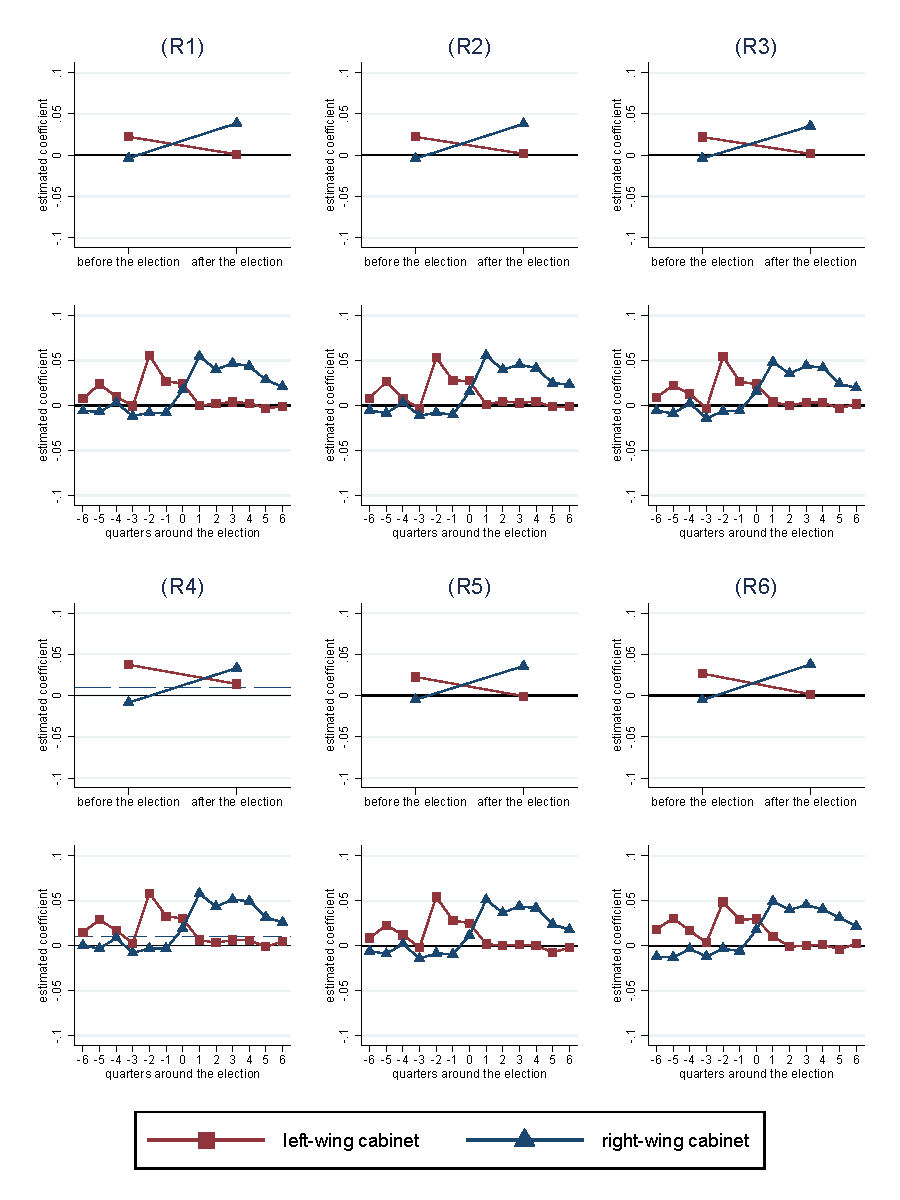
\includegraphics[width=1\textwidth]{../results/decisions/temporary_protection_rate_graphs_R1-R6.pdf}
	\scriptsize{Note: These figures show the time evolution of the temporary protection rate as estimated in fixed effects regression with a set of dummies for before and after the election or a set of dummies for different quarters before and after an election in a quarter t = 0. Significant coefficients are indicated by filled plot markers. Periods in which the two coefficients are significantly different from each other are indicated with a grey background. The navy dashed line in sub-figure R4 shows the average temporary protection rate under right-wing cabinets in periods outside the election period. Significance of the coefficients of the right-wing cabinet in sub-figure R4 is reported for the distance to this average non-election period effect.}
\end{figure}

%\clearpage
%\FloatBarrier
%\begin{table}[!ht]\centering \footnotesize
\def\sym#1{\ifmmode^{#1}\else\(^{#1}\)\fi}
\caption{Coefficients before after model temporary protection rate R1 - R2}
\begin{tabular}{l*{6}{c}}
\hline\hline
                    &\multicolumn{3}{c}{(R1)}&\multicolumn{3}{c}{(R2)}\\
&\multicolumn{1}{c}{left}&\multicolumn{1}{c}{right}&\multicolumn{1}{c}{diff}&\multicolumn{1}{c}{left}&\multicolumn{1}{c}{right}&\multicolumn{1}{c}{diff}\\
\hline
before              &      0.0223\sym{***}&    -0.00336         &      0.0257\sym{***}&      0.0223\sym{***}&    -0.00412         &      0.0264\sym{**} \\
                    &   (0.00492)         &   (0.00550)         &   (0.00776)         &   (0.00531)         &   (0.00581)         &   (0.00820)         \\
[0,5em]
after               &     0.00102         &      0.0388\sym{***}&     -0.0378\sym{***}&     0.00169         &      0.0380\sym{***}&     -0.0363\sym{***}\\
                    &   (0.00387)         &   (0.00838)         &   (0.00868)         &   (0.00399)         &   (0.00807)         &   (0.00860)         \\
\hline
Observations        &       12921         &       12921         &       12921         &       12921         &       12921         &       12921         \\
\hline\hline
\multicolumn{7}{l}{\footnotesize Standard errors in parentheses \sym{*} \(p<0.05\), \sym{**} \(p<0.01\), \sym{***} \(p<0.001\)}\\
\end{tabular}
\end{table}

%\begin{table}[htbp]\centering
\def\sym#1{\ifmmode^{#1}\else\(^{#1}\)\fi}
\caption{Coefficients quarterly model temporary\_protection\_rate R1 - R2}
\begin{tabular}{l*{6}{c}}
\hline\hline
                    &\multicolumn{1}{c}{(1)}&\multicolumn{1}{c}{(2)}&\multicolumn{1}{c}{(3)}&\multicolumn{1}{c}{(4)}&\multicolumn{1}{c}{(5)}&\multicolumn{1}{c}{(6)}\\
                    &\multicolumn{1}{c}{left2\_R1}&\multicolumn{1}{c}{right2\_R1}&\multicolumn{1}{c}{diff2\_R1}&\multicolumn{1}{c}{left2\_R2}&\multicolumn{1}{c}{right2\_R2}&\multicolumn{1}{c}{diff2\_R2}\\
\hline
 6 quarters before the election&     0.00743         &    -0.00609         &      0.0135         &     0.00817         &    -0.00537         &      0.0135         \\
                    &   (0.00813)         &   (0.00950)         &    (0.0120)         &   (0.00808)         &   (0.00961)         &    (0.0116)         \\
[1em]
 5 quarters before the election&      0.0238\sym{*}  &    -0.00694         &      0.0307\sym{*}  &      0.0264\sym{*}  &    -0.00852         &      0.0349\sym{*}  \\
                    &    (0.0103)         &   (0.00755)         &    (0.0131)         &    (0.0109)         &   (0.00773)         &    (0.0137)         \\
[1em]
 4 quarters before the election&     0.00999         &     0.00311         &     0.00688         &     0.00734         &     0.00327         &     0.00406         \\
                    &    (0.0112)         &   (0.00856)         &    (0.0132)         &    (0.0111)         &   (0.00812)         &    (0.0127)         \\
[1em]
 3 quarters before the election&   -0.000526         &     -0.0118         &      0.0113         &    -0.00294         &     -0.0113         &     0.00837         \\
                    &   (0.00890)         &   (0.00725)         &    (0.0101)         &   (0.00950)         &   (0.00681)         &   (0.00997)         \\
[1em]
 2 quarters before the election&      0.0559\sym{***}&    -0.00795         &      0.0638\sym{***}&      0.0534\sym{***}&    -0.00805         &      0.0614\sym{***}\\
                    &   (0.00871)         &   (0.00908)         &    (0.0121)         &   (0.00946)         &   (0.00916)         &    (0.0123)         \\
[1em]
 1 quarters before the election&      0.0268\sym{***}&    -0.00813         &      0.0349\sym{*}  &      0.0277\sym{***}&     -0.0102         &      0.0379\sym{*}  \\
                    &   (0.00756)         &    (0.0127)         &    (0.0151)         &   (0.00802)         &    (0.0132)         &    (0.0160)         \\
[1em]
Quarter of the election&      0.0246\sym{**} &      0.0173         &     0.00731         &      0.0275\sym{***}&      0.0153         &      0.0122         \\
                    &   (0.00783)         &    (0.0124)         &    (0.0112)         &   (0.00773)         &    (0.0127)         &    (0.0120)         \\
[1em]
 1 quarters after the election&  -0.0000703         &      0.0547\sym{***}&     -0.0547\sym{**} &     0.00117         &      0.0556\sym{***}&     -0.0544\sym{**} \\
                    &   (0.00642)         &    (0.0151)         &    (0.0171)         &   (0.00713)         &    (0.0147)         &    (0.0171)         \\
[1em]
 2 quarters after the election&     0.00189         &      0.0400\sym{**} &     -0.0381\sym{*}  &     0.00478         &      0.0397\sym{**} &     -0.0349\sym{*}  \\
                    &   (0.00696)         &    (0.0152)         &    (0.0171)         &   (0.00734)         &    (0.0149)         &    (0.0175)         \\
[1em]
 3 quarters after the election&     0.00399         &      0.0469\sym{***}&     -0.0429\sym{**} &     0.00290         &      0.0455\sym{***}&     -0.0426\sym{**} \\
                    &   (0.00555)         &    (0.0120)         &    (0.0137)         &   (0.00539)         &    (0.0116)         &    (0.0133)         \\
[1em]
 4 quarters after the election&     0.00251         &      0.0437\sym{***}&     -0.0412\sym{***}&     0.00417         &      0.0415\sym{***}&     -0.0374\sym{***}\\
                    &   (0.00614)         &   (0.00990)         &    (0.0107)         &   (0.00624)         &   (0.00991)         &    (0.0111)         \\
[1em]
 5 quarters after the election&    -0.00311         &      0.0284\sym{**} &     -0.0315\sym{**} &    -0.00148         &      0.0249\sym{*}  &     -0.0264\sym{*}  \\
                    &   (0.00596)         &    (0.0105)         &    (0.0114)         &   (0.00634)         &    (0.0104)         &    (0.0114)         \\
[1em]
 6 quarters after the election&   -0.000932         &      0.0208\sym{*}  &     -0.0218         &    -0.00145         &      0.0235\sym{*}  &     -0.0249         \\
                    &   (0.00770)         &    (0.0103)         &    (0.0131)         &   (0.00851)         &    (0.0102)         &    (0.0133)         \\
\hline
Observations        &       12921         &       12921         &       12921         &       12921         &       12921         &       12921         \\
\hline\hline
\multicolumn{7}{l}{\footnotesize Standard errors in parentheses}\\
\multicolumn{7}{l}{\footnotesize \sym{*} \(p<0.05\), \sym{**} \(p<0.01\), \sym{***} \(p<0.001\)}\\
\end{tabular}
\end{table}

%
%\clearpage
%\FloatBarrier
%\begin{table}[!ht]\centering \footnotesize
\def\sym#1{\ifmmode^{#1}\else\(^{#1}\)\fi}
\caption{Coefficients before after model temporary protection rate R3 - R4}
\begin{tabular}{l*{6}{c}}
\hline\hline
                    &\multicolumn{3}{c}{(R3)}&\multicolumn{3}{c}{(R4)}\\
&\multicolumn{1}{c}{left}&\multicolumn{1}{c}{right}&\multicolumn{1}{c}{diff}&\multicolumn{1}{c}{left}&\multicolumn{1}{c}{right}&\multicolumn{1}{c}{diff}\\
\hline
before              &      0.0221\sym{***}&    -0.00376         &      0.0258\sym{**} &      0.0275\sym{***}&    -0.00856         &      0.0265\sym{**} \\
                    &   (0.00487)         &   (0.00510)         &   (0.00796)         &   (0.00469)         &   (0.00464)         &   (0.00822)         \\
[0,5em]
after               &     0.00172         &      0.0354\sym{***}&     -0.0336\sym{***}&     0.00437         &      0.0333\sym{***}&     -0.0385\sym{***}\\
                    &   (0.00368)         &   (0.00793)         &   (0.00781)         &   (0.00530)         &   (0.00774)         &   (0.00855)         \\
\hline
Observations        &       12921         &       12921         &       12921         &       12921         &       12921         &       12921         \\
\hline\hline
\multicolumn{7}{l}{\footnotesize Standard errors in parentheses \sym{*} \(p<0.05\), \sym{**} \(p<0.01\), \sym{***} \(p<0.001\)}\\
\end{tabular}
\end{table}

%\begin{table}[htbp]\centering
\def\sym#1{\ifmmode^{#1}\else\(^{#1}\)\fi}
\caption{Coefficients quarterly model temporary\_protection\_rate R3 - R4}
\begin{tabular}{l*{6}{c}}
\hline\hline
                    &\multicolumn{1}{c}{(1)}&\multicolumn{1}{c}{(2)}&\multicolumn{1}{c}{(3)}&\multicolumn{1}{c}{(4)}&\multicolumn{1}{c}{(5)}&\multicolumn{1}{c}{(6)}\\
                    &\multicolumn{1}{c}{left2\_R3}&\multicolumn{1}{c}{right2\_R3}&\multicolumn{1}{c}{diff2\_R3}&\multicolumn{1}{c}{left2\_R4}&\multicolumn{1}{c}{right2\_R4}&\multicolumn{1}{c}{diff2\_R4}\\
\hline
 6 quarters before the election&     0.00912         &    -0.00586         &      0.0150         &      0.0151         &    -0.00967         &      0.0148         \\
                    &   (0.00749)         &   (0.00934)         &    (0.0117)         &   (0.00843)         &   (0.00791)         &    (0.0119)         \\
[1em]
 5 quarters before the election&      0.0224\sym{*}  &    -0.00884         &      0.0312\sym{*}  &      0.0288\sym{**} &     -0.0130         &      0.0319\sym{*}  \\
                    &   (0.00993)         &   (0.00724)         &    (0.0127)         &   (0.00990)         &   (0.00682)         &    (0.0129)         \\
[1em]
 4 quarters before the election&      0.0127         &     0.00240         &      0.0103         &      0.0171         &    -0.00130         &     0.00846         \\
                    &    (0.0110)         &   (0.00827)         &    (0.0139)         &    (0.0106)         &   (0.00775)         &    (0.0141)         \\
[1em]
 3 quarters before the election&    -0.00306         &     -0.0142         &      0.0111         &     0.00276         &     -0.0180\sym{*}  &      0.0108         \\
                    &   (0.00863)         &   (0.00751)         &    (0.0102)         &   (0.00917)         &   (0.00725)         &    (0.0103)         \\
[1em]
 2 quarters before the election&      0.0544\sym{***}&    -0.00629         &      0.0607\sym{***}&      0.0585\sym{***}&     -0.0128         &      0.0614\sym{***}\\
                    &   (0.00835)         &   (0.00918)         &    (0.0120)         &   (0.00740)         &   (0.00921)         &    (0.0122)         \\
[1em]
 1 quarters before the election&      0.0264\sym{***}&    -0.00595         &      0.0324\sym{*}  &      0.0330\sym{***}&     -0.0131         &      0.0362\sym{*}  \\
                    &   (0.00719)         &    (0.0112)         &    (0.0141)         &   (0.00793)         &    (0.0112)         &    (0.0146)         \\
[1em]
Quarter of the election&      0.0238\sym{**} &      0.0155         &     0.00830         &      0.0303\sym{***}&     0.00924         &      0.0111         \\
                    &   (0.00837)         &    (0.0118)         &    (0.0107)         &   (0.00776)         &    (0.0126)         &    (0.0110)         \\
[1em]
 1 quarters after the election&     0.00397         &      0.0483\sym{***}&     -0.0443\sym{**} &     0.00638         &      0.0482\sym{***}&     -0.0517\sym{**} \\
                    &   (0.00667)         &    (0.0144)         &    (0.0163)         &   (0.00684)         &    (0.0146)         &    (0.0172)         \\
[1em]
 2 quarters after the election&   -0.000211         &      0.0352\sym{*}  &     -0.0355\sym{*}  &     0.00342         &      0.0335\sym{*}  &     -0.0401\sym{*}  \\
                    &   (0.00640)         &    (0.0147)         &    (0.0161)         &   (0.00755)         &    (0.0145)         &    (0.0169)         \\
[1em]
 3 quarters after the election&     0.00352         &      0.0441\sym{***}&     -0.0406\sym{***}&     0.00651         &      0.0414\sym{***}&     -0.0449\sym{***}\\
                    &   (0.00551)         &    (0.0110)         &    (0.0122)         &   (0.00663)         &    (0.0110)         &    (0.0124)         \\
[1em]
 4 quarters after the election&     0.00305         &      0.0420\sym{***}&     -0.0390\sym{***}&     0.00617         &      0.0396\sym{***}&     -0.0434\sym{***}\\
                    &   (0.00568)         &   (0.00948)         &   (0.00998)         &   (0.00715)         &   (0.00985)         &    (0.0103)         \\
[1em]
 5 quarters after the election&    -0.00317         &      0.0241\sym{*}  &     -0.0272\sym{**} &    -0.00114         &      0.0218\sym{*}  &     -0.0329\sym{**} \\
                    &   (0.00532)         &    (0.0102)         &    (0.0104)         &   (0.00745)         &   (0.00981)         &    (0.0114)         \\
[1em]
 6 quarters after the election&     0.00175         &      0.0196\sym{*}  &     -0.0178         &     0.00477         &      0.0161         &     -0.0213         \\
                    &   (0.00776)         &   (0.00980)         &    (0.0119)         &   (0.00866)         &   (0.00904)         &    (0.0120)         \\
\hline
Observations        &       12921         &       12921         &       12921         &       12921         &       12921         &       12921         \\
\hline\hline
\multicolumn{7}{l}{\footnotesize Standard errors in parentheses}\\
\multicolumn{7}{l}{\footnotesize \sym{*} \(p<0.05\), \sym{**} \(p<0.01\), \sym{***} \(p<0.001\)}\\
\end{tabular}
\end{table}

%
%\clearpage
%\FloatBarrier
%\begin{table}[!ht]\centering \footnotesize
\def\sym#1{\ifmmode^{#1}\else\(^{#1}\)\fi}
\caption{Coefficients before after model temporary protection rate R5 - R6}
\begin{tabular}{l*{6}{c}}
\hline\hline
                    &\multicolumn{3}{c}{(R5)}&\multicolumn{3}{c}{(R6)}\\
&\multicolumn{1}{c}{left}&\multicolumn{1}{c}{right}&\multicolumn{1}{c}{diff}&\multicolumn{1}{c}{left}&\multicolumn{1}{c}{right}&\multicolumn{1}{c}{diff}\\
\hline
before              &      0.0225\sym{***}&    -0.00503         &      0.0276\sym{***}&      0.0266\sym{***}&    -0.00540         &      0.0320\sym{***}\\
                    &   (0.00487)         &   (0.00513)         &   (0.00803)         &   (0.00509)         &   (0.00504)         &   (0.00815)         \\
[0,5em]
after               &   -0.000823         &      0.0357\sym{***}&     -0.0365\sym{***}&     0.00151         &      0.0378\sym{***}&     -0.0362\sym{***}\\
                    &   (0.00362)         &   (0.00849)         &   (0.00879)         &   (0.00355)         &   (0.00863)         &   (0.00881)         \\
\hline
Observations        &       12921         &       12921         &       12921         &       12921         &       12921         &       12921         \\
\hline\hline
\multicolumn{7}{l}{\footnotesize Standard errors in parentheses \sym{*} \(p<0.05\), \sym{**} \(p<0.01\), \sym{***} \(p<0.001\)}\\
\end{tabular}
\end{table}

%\begin{table}[htbp]\centering
\def\sym#1{\ifmmode^{#1}\else\(^{#1}\)\fi}
\caption{Coefficients quarterly model temporary\_protection\_rate R5 - R6}
\begin{tabular}{l*{6}{c}}
\hline\hline
                    &\multicolumn{1}{c}{(1)}&\multicolumn{1}{c}{(2)}&\multicolumn{1}{c}{(3)}&\multicolumn{1}{c}{(4)}&\multicolumn{1}{c}{(5)}&\multicolumn{1}{c}{(6)}\\
                    &\multicolumn{1}{c}{left2\_R5}&\multicolumn{1}{c}{right2\_R5}&\multicolumn{1}{c}{diff2\_R5}&\multicolumn{1}{c}{left2\_R6}&\multicolumn{1}{c}{right2\_R6}&\multicolumn{1}{c}{diff2\_R6}\\
\hline
 6 quarters before the election&     0.00872         &    -0.00591         &      0.0146         &      0.0183\sym{*}  &     -0.0121         &      0.0304\sym{*}  \\
                    &   (0.00773)         &   (0.00931)         &    (0.0119)         &   (0.00869)         &   (0.00956)         &    (0.0134)         \\
[1em]
 5 quarters before the election&      0.0229\sym{*}  &    -0.00901         &      0.0319\sym{*}  &      0.0307\sym{**} &     -0.0129         &      0.0436\sym{**} \\
                    &   (0.00999)         &   (0.00729)         &    (0.0127)         &    (0.0108)         &   (0.00739)         &    (0.0137)         \\
[1em]
 4 quarters before the election&      0.0120         &     0.00198         &     0.00998         &      0.0168         &    -0.00348         &      0.0203         \\
                    &    (0.0110)         &   (0.00829)         &    (0.0139)         &    (0.0110)         &   (0.00862)         &    (0.0140)         \\
[1em]
 3 quarters before the election&    -0.00171         &     -0.0142         &      0.0125         &     0.00343         &     -0.0120         &      0.0154         \\
                    &   (0.00847)         &   (0.00746)         &    (0.0101)         &   (0.00837)         &   (0.00716)         &    (0.0102)         \\
[1em]
 2 quarters before the election&      0.0542\sym{***}&    -0.00848         &      0.0627\sym{***}&      0.0487\sym{***}&    -0.00322         &      0.0520\sym{***}\\
                    &   (0.00841)         &   (0.00925)         &    (0.0120)         &   (0.00824)         &   (0.00920)         &    (0.0119)         \\
[1em]
 1 quarters before the election&      0.0282\sym{***}&    -0.00928         &      0.0375\sym{**} &      0.0289\sym{***}&    -0.00596         &      0.0349\sym{**} \\
                    &   (0.00718)         &    (0.0116)         &    (0.0145)         &   (0.00715)         &    (0.0106)         &    (0.0134)         \\
[1em]
Quarter of the election&      0.0251\sym{**} &      0.0117         &      0.0133         &      0.0298\sym{***}&      0.0176         &      0.0122         \\
                    &   (0.00828)         &    (0.0118)         &    (0.0107)         &   (0.00836)         &    (0.0114)         &   (0.00966)         \\
[1em]
 1 quarters after the election&     0.00186         &      0.0512\sym{***}&     -0.0493\sym{**} &      0.0105         &      0.0495\sym{***}&     -0.0390\sym{*}  \\
                    &   (0.00671)         &    (0.0150)         &    (0.0173)         &   (0.00646)         &    (0.0148)         &    (0.0168)         \\
[1em]
 2 quarters after the election&    0.000284         &      0.0366\sym{*}  &     -0.0363\sym{*}  &   -0.000976         &      0.0399\sym{**} &     -0.0409\sym{*}  \\
                    &   (0.00671)         &    (0.0152)         &    (0.0172)         &   (0.00661)         &    (0.0152)         &    (0.0174)         \\
[1em]
 3 quarters after the election&     0.00130         &      0.0439\sym{***}&     -0.0426\sym{***}&   0.0000320         &      0.0454\sym{***}&     -0.0454\sym{***}\\
                    &   (0.00530)         &    (0.0116)         &    (0.0127)         &   (0.00543)         &    (0.0116)         &    (0.0128)         \\
[1em]
 4 quarters after the election&    0.000383         &      0.0419\sym{***}&     -0.0415\sym{***}&     0.00119         &      0.0405\sym{***}&     -0.0393\sym{***}\\
                    &   (0.00573)         &   (0.00984)         &    (0.0104)         &   (0.00560)         &    (0.0101)         &    (0.0104)         \\
[1em]
 5 quarters after the election&    -0.00746         &      0.0239\sym{*}  &     -0.0313\sym{**} &    -0.00407         &      0.0312\sym{**} &     -0.0352\sym{**} \\
                    &   (0.00543)         &    (0.0108)         &    (0.0116)         &   (0.00538)         &    (0.0110)         &    (0.0117)         \\
[1em]
 6 quarters after the election&    -0.00219         &      0.0178         &     -0.0200         &     0.00241         &      0.0219\sym{*}  &     -0.0195         \\
                    &   (0.00731)         &   (0.00985)         &    (0.0121)         &   (0.00774)         &    (0.0100)         &    (0.0125)         \\
\hline
Observations        &       12921         &       12921         &       12921         &       12921         &       12921         &       12921         \\
\hline\hline
\multicolumn{7}{l}{\footnotesize Standard errors in parentheses}\\
\multicolumn{7}{l}{\footnotesize \sym{*} \(p<0.05\), \sym{**} \(p<0.01\), \sym{***} \(p<0.001\)}\\
\end{tabular}
\end{table}




\clearpage
\FloatBarrier
\begin{table}[!ht]\centering \scriptsize
	\def\sym#1{\ifmmode^{#1}\else\(^{#1}\)\fi}
	\caption{Determinants of temporary protection rate - R7 - R12}
	\begin{tabular}{l*{6}{c}}
		\hline\hline
		&\multicolumn{1}{c}{(1)}     &\multicolumn{1}{c}{(2)}       &\multicolumn{1}{c}{(3)}       &\multicolumn{1}{c}{(4)}    	&\multicolumn{1}{c}{(5)}  	&\multicolumn{1}{c}{(6)}   \\
		&\multicolumn{1}{c}{R7}&\multicolumn{1}{c}{R8}&\multicolumn{1}{c}{R9}&\multicolumn{1}{c}{R10}&\multicolumn{1}{c}{R11}&\multicolumn{1}{c}{R12}\\ 

\hline
Political Terror Scale&    -0.00255         &                     &    -0.00257         &    -0.00257         &    -0.00257         &    -0.00195         \\
                    &   (0.00648)         &                     &   (0.00579)         &   (0.00628)         &   (0.00628)         &   (0.00569)         \\
[0,5em]
Civic Liberty (FHI) &      0.0127         &                     &      0.0125         &      0.0125         &      0.0125         &      0.0174         \\
                    &   (0.00991)         &                     &   (0.00750)         &   (0.00994)         &   (0.00994)         &   (0.00944)         \\
[0,5em]
Political Rights (FHI)&     0.00158         &                     &     0.00161         &     0.00161         &     0.00161         &    -0.00125         \\
                    &   (0.00928)         &                     &   (0.00696)         &   (0.00923)         &   (0.00923)         &   (0.00827)         \\
[0,5em]
Quarterly civil war &      0.0371\sym{***}&                     &      0.0372\sym{***}&      0.0372\sym{***}&      0.0372\sym{***}&      0.0314\sym{***}\\
battle death (000s)                    &   (0.00291)         &                     &   (0.00858)         &   (0.00264)         &   (0.00264)         &   (0.00225)         \\
[0,5em]
Log origin country real &    -0.00813         &                     &    -0.00795         &    -0.00795         &    -0.00795         &    -0.00460         \\
GDP per capita                    &    (0.0129)         &                     &    (0.0161)         &    (0.0125)         &    (0.0125)         &    (0.0181)         \\
[0,5em]
Log destination country quarterly &       0.358\sym{***}&       0.338\sym{***}&       0.369\sym{***}&       0.369\sym{***}&       0.369\sym{***}&       0.252\sym{***}\\
real GDP per capita                    &    (0.0773)         &    (0.0790)         &    (0.0740)         &    (0.0814)         &    (0.0814)         &    (0.0625)         \\
[0,5em]
Quarterly unemployment rate&     0.00360\sym{*}  &     0.00315\sym{*}  &     0.00424\sym{**} &     0.00424\sym{*}  &     0.00424\sym{*}  &     0.00291\sym{*}  \\
 at destination                    &   (0.00159)         &   (0.00155)         &   (0.00161)         &   (0.00166)         &   (0.00166)         &   (0.00121)         \\
[0,5em]
Log total decisions per capita &    -0.00818         &                     &                     &                     &                     &                     \\
in previous year                    &   (0.00917)         &                     &                     &                     &                     &                     \\
[0,5em]
Log dyadic decisions at destination &    0.000129         &                     &                     &                     &                     &                     \\
per capita in previous year                    &   (0.00401)         &                     &                     &                     &                     &                     \\
[0,5em]
Log total first-time applications&                     &     -0.0162         &                     &                     &                     &                     \\
 in the previous 2 quarters                    &                     &   (0.00868)         &                     &                     &                     &                     \\
[0,5em]
Log dyadic first-time applications &                     &     0.00310         &                     &                     &                     &                     \\
in the previous 2 quarters                    &                     &   (0.00679)         &                     &                     &                     &                     \\
[0,5em]
Years after 2007    &                     &                     &                     &     -0.0360\sym{*}  &                     &                     \\
                    &                     &                     &                     &    (0.0178)         &                     &                     \\
[0,5em]
Cabinet position left * &      0.0226\sym{***}&      0.0220\sym{***}&      0.0223\sym{***}&      0.0223\sym{***}&      0.0223\sym{***}&      0.0158\sym{**} \\
Before the election                    &   (0.00478)         &   (0.00493)         &   (0.00588)         &   (0.00483)         &   (0.00483)         &   (0.00465)         \\
[0,5em]
Cabinet position left * &    0.000989         &     0.00149         &    0.000205         &    0.000205         &    0.000205         &     0.00264         \\
After the election                    &   (0.00371)         &   (0.00363)         &   (0.00474)         &   (0.00377)         &   (0.00377)         &   (0.00281)         \\
[0,5em]
Cabinet position right * &    -0.00465         &    -0.00486         &    -0.00433         &    -0.00433         &    -0.00433         &     -0.0121\sym{**} \\
Before the election                    &   (0.00518)         &   (0.00504)         &   (0.00519)         &   (0.00518)         &   (0.00518)         &   (0.00434)         \\
[0,5em]
Cabinet position right * &      0.0371\sym{***}&      0.0360\sym{***}&      0.0375\sym{***}&      0.0375\sym{***}&      0.0375\sym{***}&      0.0239\sym{***}\\
After the election                    &   (0.00804)         &   (0.00812)         &   (0.00677)         &   (0.00824)         &   (0.00824)         &   (0.00525)         \\
\hline
Observations        &       12921         &       12868         &       12921         &       12921         &       12921         &       17191         \\
Adjusted \(R^{2}\)  &       0.067         &       0.035         &       0.067         &       0.067         &       0.067         &       0.046         \\
Mean temporary\_protection\_rate&      0.0725         &      0.0726         &      0.0725         &      0.0725         &      0.0725         &      0.0779         \\
Fixed Effects       &       D x O         &       D x O         &       D x O         &       D x O         &       D x O         &       D x O         \\
Destination dummies &          No         &          No         &          No         &          No         &          No         &          No         \\
Quarter-Year dummies&         Yes         &         Yes         &         Yes         &         Yes         &         Yes         &         Yes         \\
\hline\hline
\multicolumn{7}{l}{ Standard errors in parentheses \sym{*} \(p<0.05\), \sym{**} \(p<0.01\), \sym{***} \(p<0.001\)}\\
\end{tabular}
\end{table}


\clearpage
\FloatBarrier
\begin{figure}[!ht]
	\caption{Temporary protection decisions per capita: predicted pattern - R7 to R12}
	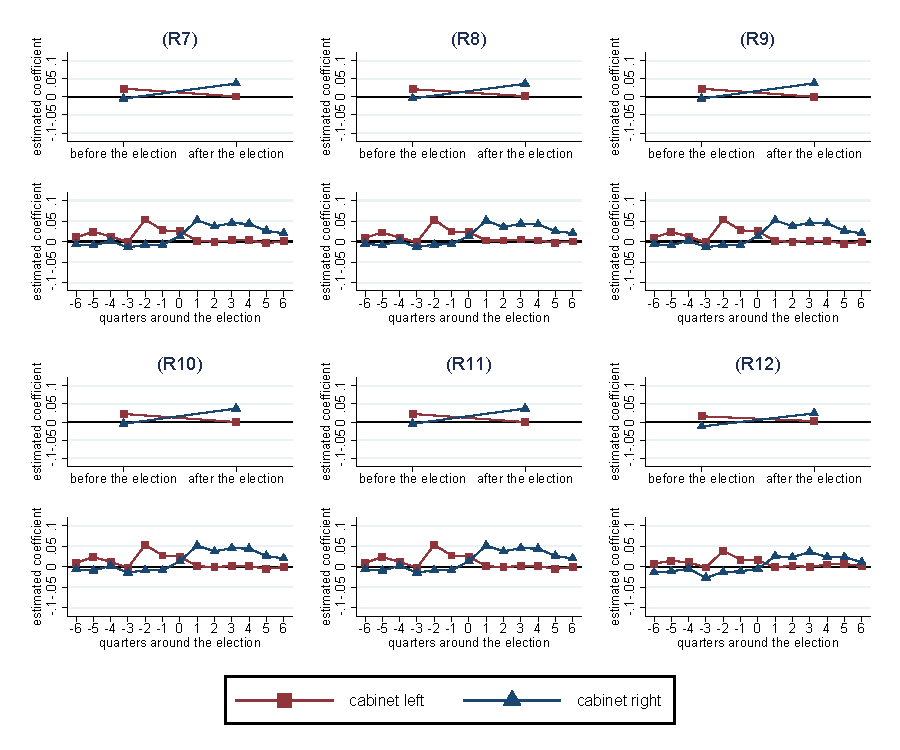
\includegraphics[width=1\textwidth]{../results/decisions/temporary_protection_rate_graphs_R7-R12.pdf}
	\scriptsize{Note: These figures show the time evolution of the temporary protection rate as estimated in fixed effects regression with a set of dummies for before and after the election or a set of dummies for different quarters before and after an election in a quarter t = 0. Significant coefficients are indicated by filled plot markers. Periods in which the two coefficients are significantly different from each other are indicated with a grey background.}
\end{figure}

%\clearpage
%\FloatBarrier
%\begin{table}[!ht]\centering \footnotesize
\def\sym#1{\ifmmode^{#1}\else\(^{#1}\)\fi}
\caption{Coefficients before after model temporary\_protection\_rate R7 - R8}
\begin{tabular}{l*{6}{c}}
\hline\hline
                    &\multicolumn{1}{c}{(1)}&\multicolumn{1}{c}{(2)}&\multicolumn{1}{c}{(3)}&\multicolumn{1}{c}{(4)}&\multicolumn{1}{c}{(5)}&\multicolumn{1}{c}{(6)}\\
                    &\multicolumn{1}{c}{left1\_R7}&\multicolumn{1}{c}{right1\_R7}&\multicolumn{1}{c}{diff1\_R7}&\multicolumn{1}{c}{left1\_R8}&\multicolumn{1}{c}{right1\_R8}&\multicolumn{1}{c}{diff1\_R8}\\
\hline
before              &      0.0226\sym{***}&    -0.00465         &      0.0273\sym{***}&      0.0210\sym{***}&    -0.00406         &      0.0251\sym{**} \\
                    &   (0.00478)         &   (0.00518)         &   (0.00797)         &   (0.00487)         &   (0.00511)         &   (0.00798)         \\
[1em]
after               &    0.000989         &      0.0371\sym{***}&     -0.0361\sym{***}&     0.00199         &      0.0362\sym{***}&     -0.0342\sym{***}\\
                    &   (0.00371)         &   (0.00804)         &   (0.00778)         &   (0.00366)         &   (0.00795)         &   (0.00760)         \\
\hline
Observations        &       12921         &       12921         &       12921         &       12868         &       12868         &       12868         \\
\hline\hline
\multicolumn{7}{l}{\footnotesize Standard errors in parentheses}\\
\multicolumn{7}{l}{\footnotesize \sym{*} \(p<0.05\), \sym{**} \(p<0.01\), \sym{***} \(p<0.001\)}\\
\end{tabular}
\end{table}

%\begin{table}[htbp]\centering
\def\sym#1{\ifmmode^{#1}\else\(^{#1}\)\fi}
\caption{Coefficients quarterly model temporary\_protection\_rate R7 - R8}
\begin{tabular}{l*{6}{c}}
\hline\hline
                    &\multicolumn{1}{c}{(1)}&\multicolumn{1}{c}{(2)}&\multicolumn{1}{c}{(3)}&\multicolumn{1}{c}{(4)}&\multicolumn{1}{c}{(5)}&\multicolumn{1}{c}{(6)}\\
                    &\multicolumn{1}{c}{left2\_R7}&\multicolumn{1}{c}{right2\_R7}&\multicolumn{1}{c}{diff2\_R7}&\multicolumn{1}{c}{left2\_R8}&\multicolumn{1}{c}{right2\_R8}&\multicolumn{1}{c}{diff2\_R8}\\
\hline
 6 quarters before the election&      0.0102         &    -0.00707         &      0.0172         &     0.00936         &    -0.00572         &      0.0151         \\
                    &   (0.00778)         &   (0.00914)         &    (0.0118)         &   (0.00776)         &   (0.00914)         &    (0.0117)         \\
[1em]
 5 quarters before the election&      0.0239\sym{*}  &    -0.00960         &      0.0335\sym{**} &      0.0221\sym{*}  &    -0.00854         &      0.0306\sym{*}  \\
                    &    (0.0100)         &   (0.00730)         &    (0.0128)         &   (0.00996)         &   (0.00736)         &    (0.0128)         \\
[1em]
 4 quarters before the election&      0.0125         &     0.00143         &      0.0110         &     0.00948         &    0.000861         &     0.00862         \\
                    &    (0.0110)         &   (0.00827)         &    (0.0138)         &    (0.0110)         &   (0.00828)         &    (0.0139)         \\
[1em]
 3 quarters before the election&    -0.00144         &     -0.0144         &      0.0130         &    -0.00137         &     -0.0136         &      0.0122         \\
                    &   (0.00825)         &   (0.00754)         &    (0.0101)         &   (0.00818)         &   (0.00732)         &    (0.0100)         \\
[1em]
 2 quarters before the election&      0.0539\sym{***}&    -0.00809         &      0.0620\sym{***}&      0.0532\sym{***}&    -0.00757         &      0.0607\sym{***}\\
                    &   (0.00821)         &   (0.00930)         &    (0.0120)         &   (0.00837)         &   (0.00924)         &    (0.0120)         \\
[1em]
 1 quarters before the election&      0.0273\sym{***}&    -0.00761         &      0.0349\sym{*}  &      0.0246\sym{***}&    -0.00611         &      0.0307\sym{*}  \\
                    &   (0.00724)         &    (0.0115)         &    (0.0144)         &   (0.00734)         &    (0.0113)         &    (0.0143)         \\
[1em]
Quarter of the election&      0.0249\sym{**} &      0.0136         &      0.0113         &      0.0229\sym{**} &      0.0136         &     0.00935         \\
                    &   (0.00820)         &    (0.0119)         &    (0.0109)         &   (0.00802)         &    (0.0120)         &    (0.0109)         \\
[1em]
 1 quarters after the election&     0.00197         &      0.0517\sym{***}&     -0.0497\sym{**} &     0.00260         &      0.0511\sym{***}&     -0.0485\sym{**} \\
                    &   (0.00661)         &    (0.0149)         &    (0.0168)         &   (0.00664)         &    (0.0147)         &    (0.0165)         \\
[1em]
 2 quarters after the election&   -0.000375         &      0.0369\sym{*}  &     -0.0373\sym{*}  &     0.00254         &      0.0351\sym{*}  &     -0.0326\sym{*}  \\
                    &   (0.00640)         &    (0.0148)         &    (0.0161)         &   (0.00637)         &    (0.0147)         &    (0.0157)         \\
[1em]
 3 quarters after the election&     0.00317         &      0.0450\sym{***}&     -0.0419\sym{***}&     0.00501         &      0.0437\sym{***}&     -0.0387\sym{***}\\
                    &   (0.00545)         &    (0.0111)         &    (0.0121)         &   (0.00565)         &    (0.0108)         &    (0.0115)         \\
[1em]
 4 quarters after the election&     0.00281         &      0.0432\sym{***}&     -0.0403\sym{***}&     0.00278         &      0.0419\sym{***}&     -0.0391\sym{***}\\
                    &   (0.00594)         &   (0.00948)         &   (0.00994)         &   (0.00587)         &   (0.00944)         &    (0.0102)         \\
[1em]
 5 quarters after the election&    -0.00412         &      0.0261\sym{*}  &     -0.0302\sym{**} &    -0.00305         &      0.0250\sym{*}  &     -0.0280\sym{**} \\
                    &   (0.00551)         &    (0.0104)         &    (0.0105)         &   (0.00540)         &    (0.0105)         &    (0.0105)         \\
[1em]
 6 quarters after the election&    0.000485         &      0.0202\sym{*}  &     -0.0197         &   0.0000716         &      0.0207\sym{*}  &     -0.0206         \\
                    &   (0.00759)         &   (0.00976)         &    (0.0117)         &   (0.00762)         &   (0.00993)         &    (0.0119)         \\
\hline
Observations        &       12921         &       12921         &       12921         &       12868         &       12868         &       12868         \\
\hline\hline
\multicolumn{7}{l}{\footnotesize Standard errors in parentheses}\\
\multicolumn{7}{l}{\footnotesize \sym{*} \(p<0.05\), \sym{**} \(p<0.01\), \sym{***} \(p<0.001\)}\\
\end{tabular}
\end{table}

%
%\clearpage
%\FloatBarrier
%\begin{table}[!ht]\centering \footnotesize
\def\sym#1{\ifmmode^{#1}\else\(^{#1}\)\fi}
\caption{Coefficients before after model temporary protection rate R9 - R10}
\begin{tabular}{l*{6}{c}}
\hline\hline
                    &\multicolumn{3}{c}{(R9)}&\multicolumn{3}{c}{(R10)}\\
&\multicolumn{1}{c}{left}&\multicolumn{1}{c}{right}&\multicolumn{1}{c}{diff}&\multicolumn{1}{c}{left}&\multicolumn{1}{c}{right}&\multicolumn{1}{c}{diff}\\
\hline
before              &      0.0225\sym{***}&    -0.00469         &      0.0272\sym{**} &      0.0225\sym{***}&    -0.00469         &      0.0272\sym{***}\\
                    &   (0.00588)         &   (0.00522)         &   (0.00863)         &   (0.00483)         &   (0.00519)         &   (0.00801)         \\
[0,5em]
after               &   0.0000830         &      0.0373\sym{***}&     -0.0372\sym{***}&   0.0000830         &      0.0373\sym{***}&     -0.0372\sym{***}\\
                    &   (0.00475)         &   (0.00675)         &   (0.00792)         &   (0.00377)         &   (0.00823)         &   (0.00839)         \\
\hline
Observations        &       12921         &       12921         &       12921         &       12921         &       12921         &       12921         \\
\hline\hline
\multicolumn{7}{l}{\footnotesize Standard errors in parentheses \sym{*} \(p<0.05\), \sym{**} \(p<0.01\), \sym{***} \(p<0.001\)}\\
\end{tabular}
\end{table}

%\begin{table}[!ht]\centering \footnotesize
\def\sym#1{\ifmmode^{#1}\else\(^{#1}\)\fi}
\caption{Coefficients quarterly model temporary\_protection\_rate R9 - R10}
\begin{tabular}{l*{6}{c}}
\hline\hline
                    &\multicolumn{1}{c}{(1)}&\multicolumn{1}{c}{(2)}&\multicolumn{1}{c}{(3)}&\multicolumn{1}{c}{(4)}&\multicolumn{1}{c}{(5)}&\multicolumn{1}{c}{(6)}\\
                    &\multicolumn{1}{c}{left2\_R9}&\multicolumn{1}{c}{right2\_R9}&\multicolumn{1}{c}{diff2\_R9}&\multicolumn{1}{c}{left2\_R10}&\multicolumn{1}{c}{right2\_R10}&\multicolumn{1}{c}{diff2\_R10}\\
\hline
 6 quarters before the election&     0.00990         &    -0.00576         &      0.0157         &     0.00990         &    -0.00576         &      0.0157         \\
                    &   (0.00866)         &   (0.00863)         &    (0.0124)         &   (0.00771)         &   (0.00919)         &    (0.0117)         \\
[1em]
 5 quarters before the election&      0.0236\sym{*}  &    -0.00878         &      0.0323\sym{*}  &      0.0236\sym{*}  &    -0.00878         &      0.0323\sym{*}  \\
                    &   (0.00960)         &   (0.00887)         &    (0.0143)         &    (0.0100)         &   (0.00732)         &    (0.0128)         \\
[1em]
 4 quarters before the election&      0.0114         &     0.00235         &     0.00906         &      0.0114         &     0.00235         &     0.00906         \\
                    &    (0.0109)         &   (0.00776)         &    (0.0129)         &    (0.0110)         &   (0.00830)         &    (0.0139)         \\
[1em]
 3 quarters before the election&    -0.00180         &     -0.0137         &      0.0119         &    -0.00180         &     -0.0137         &      0.0119         \\
                    &    (0.0101)         &   (0.00781)         &    (0.0117)         &   (0.00843)         &   (0.00743)         &    (0.0101)         \\
[1em]
 2 quarters before the election&      0.0536\sym{***}&    -0.00751         &      0.0612\sym{***}&      0.0536\sym{***}&    -0.00751         &      0.0612\sym{***}\\
                    &    (0.0116)         &   (0.00883)         &    (0.0149)         &   (0.00834)         &   (0.00923)         &    (0.0120)         \\
[1em]
 1 quarters before the election&      0.0270\sym{**} &    -0.00784         &      0.0349\sym{*}  &      0.0270\sym{***}&    -0.00784         &      0.0349\sym{*}  \\
                    &   (0.00936)         &    (0.0104)         &    (0.0146)         &   (0.00726)         &    (0.0115)         &    (0.0144)         \\
[1em]
Quarter of the election&      0.0244\sym{**} &      0.0134         &      0.0110         &      0.0244\sym{**} &      0.0134         &      0.0110         \\
                    &   (0.00802)         &   (0.00958)         &    (0.0116)         &   (0.00819)         &    (0.0120)         &    (0.0110)         \\
[1em]
 1 quarters after the election&     0.00189         &      0.0523\sym{***}&     -0.0504\sym{***}&     0.00189         &      0.0523\sym{***}&     -0.0504\sym{**} \\
                    &   (0.00662)         &    (0.0125)         &    (0.0142)         &   (0.00660)         &    (0.0148)         &    (0.0168)         \\
[1em]
 2 quarters after the election&   -0.000791         &      0.0379\sym{**} &     -0.0387\sym{**} &   -0.000791         &      0.0379\sym{*}  &     -0.0387\sym{*}  \\
                    &   (0.00766)         &    (0.0132)         &    (0.0148)         &   (0.00645)         &    (0.0150)         &    (0.0166)         \\
[1em]
 3 quarters after the election&     0.00201         &      0.0459\sym{***}&     -0.0439\sym{***}&     0.00201         &      0.0459\sym{***}&     -0.0439\sym{***}\\
                    &   (0.00640)         &    (0.0113)         &    (0.0125)         &   (0.00538)         &    (0.0112)         &    (0.0124)         \\
[1em]
 4 quarters after the election&     0.00174         &      0.0436\sym{***}&     -0.0419\sym{**} &     0.00174         &      0.0436\sym{***}&     -0.0419\sym{***}\\
                    &   (0.00738)         &    (0.0107)         &    (0.0132)         &   (0.00591)         &   (0.00974)         &    (0.0103)         \\
[1em]
 5 quarters after the election&    -0.00486         &      0.0267\sym{**} &     -0.0316\sym{**} &    -0.00486         &      0.0267\sym{*}  &     -0.0316\sym{**} \\
                    &   (0.00645)         &   (0.00964)         &    (0.0118)         &   (0.00564)         &    (0.0105)         &    (0.0113)         \\
[1em]
 6 quarters after the election&   0.0000448         &      0.0206\sym{*}  &     -0.0206         &   0.0000448         &      0.0206\sym{*}  &     -0.0206         \\
                    &   (0.00814)         &   (0.00970)         &    (0.0127)         &   (0.00768)         &   (0.00971)         &    (0.0120)         \\
\hline
Observations        &       12921         &       12921         &       12921         &       12921         &       12921         &       12921         \\
\hline\hline
\multicolumn{7}{l}{\footnotesize Standard errors in parentheses}\\
\multicolumn{7}{l}{\footnotesize \sym{*} \(p<0.05\), \sym{**} \(p<0.01\), \sym{***} \(p<0.001\)}\\
\end{tabular}
\end{table}

%
%\clearpage
%\FloatBarrier
%\begin{table}[!ht]\centering \footnotesize
\def\sym#1{\ifmmode^{#1}\else\(^{#1}\)\fi}
\caption{Coefficients before after model temporary protection rate R11 - R12}
\begin{tabular}{l*{6}{c}}
\hline\hline
                    &\multicolumn{3}{c}{(R11)}&\multicolumn{3}{c}{(R12)}\\
&\multicolumn{1}{c}{left}&\multicolumn{1}{c}{right}&\multicolumn{1}{c}{diff}&\multicolumn{1}{c}{left}&\multicolumn{1}{c}{right}&\multicolumn{1}{c}{diff}\\
\hline
before              &      0.0225\sym{***}&    -0.00469         &      0.0272\sym{***}&      0.0159\sym{***}&     -0.0121\sym{**} &      0.0280\sym{***}\\
                    &   (0.00483)         &   (0.00519)         &   (0.00801)         &   (0.00466)         &   (0.00435)         &   (0.00752)         \\
[0,5em]
after               &   0.0000830         &      0.0373\sym{***}&     -0.0372\sym{***}&     0.00271         &      0.0239\sym{***}&     -0.0212\sym{***}\\
                    &   (0.00377)         &   (0.00823)         &   (0.00839)         &   (0.00279)         &   (0.00527)         &   (0.00578)         \\
\hline
Observations        &       12921         &       12921         &       12921         &       17191         &       17191         &       17191         \\
\hline\hline
\multicolumn{7}{l}{\footnotesize Standard errors in parentheses \sym{*} \(p<0.05\), \sym{**} \(p<0.01\), \sym{***} \(p<0.001\)}\\
\end{tabular}
\end{table}

%\begin{table}[!ht]\centering \footnotesize
\def\sym#1{\ifmmode^{#1}\else\(^{#1}\)\fi}
\caption{Coefficients quarterly model temporary protection rate R11 - R12}
\begin{tabular}{l*{6}{c}}
\hline\hline
                    &\multicolumn{3}{c}{(R11)}&\multicolumn{3}{c}{(R12)}\\
&\multicolumn{1}{c}{left}&\multicolumn{1}{c}{right}&\multicolumn{1}{c}{diff}&\multicolumn{1}{c}{left}&\multicolumn{1}{c}{right}&\multicolumn{1}{c}{diff}\\
\hline
 6 quarters before the election&     0.00977         &    -0.00624         &      0.0160         &     0.00779         &     -0.0136         &      0.0214\sym{*}  \\
                    &   (0.00770)         &   (0.00921)         &    (0.0117)         &   (0.00635)         &   (0.00776)         &   (0.00918)         \\
[0,5em]
 5 quarters before the election&      0.0235\sym{*}  &    -0.00919         &      0.0327\sym{*}  &      0.0147         &     -0.0111\sym{*}  &      0.0258\sym{*}  \\
                    &    (0.0100)         &   (0.00732)         &    (0.0128)         &   (0.00955)         &   (0.00513)         &    (0.0107)         \\
[0,5em]
 4 quarters before the election&      0.0121         &     0.00249         &     0.00961         &      0.0108         &    -0.00479         &      0.0156         \\
                    &    (0.0110)         &   (0.00825)         &    (0.0138)         &   (0.00909)         &   (0.00815)         &    (0.0120)         \\
[0,5em]
 3 quarters before the election&    -0.00210         &     -0.0140         &      0.0119         &    -0.00158         &     -0.0268\sym{***}&      0.0253\sym{**} \\
                    &   (0.00845)         &   (0.00747)         &    (0.0101)         &   (0.00742)         &   (0.00583)         &   (0.00864)         \\
[0,5em]
 2 quarters before the election&      0.0536\sym{***}&    -0.00832         &      0.0619\sym{***}&      0.0388\sym{***}&     -0.0125         &      0.0513\sym{***}\\
                    &   (0.00832)         &   (0.00929)         &    (0.0121)         &   (0.00818)         &   (0.00914)         &    (0.0128)         \\
[0,5em]
 1 quarters before the election&      0.0274\sym{***}&    -0.00865         &      0.0360\sym{*}  &      0.0175\sym{**} &     -0.0111         &      0.0286\sym{**} \\
                    &   (0.00724)         &    (0.0116)         &    (0.0146)         &   (0.00618)         &   (0.00839)         &    (0.0107)         \\
[0,5em]
Quarter of the election&      0.0247\sym{**} &      0.0135         &      0.0113         &      0.0162\sym{*}  &    -0.00484         &      0.0210\sym{*}  \\
                    &   (0.00822)         &    (0.0120)         &    (0.0110)         &   (0.00807)         &   (0.00791)         &    (0.0103)         \\
[0,5em]
 1 quarters after the election&     0.00163         &      0.0517\sym{***}&     -0.0501\sym{**} &   -0.000783         &      0.0259\sym{**} &     -0.0267\sym{*}  \\
                    &   (0.00663)         &    (0.0148)         &    (0.0168)         &   (0.00618)         &   (0.00969)         &    (0.0126)         \\
[0,5em]
 2 quarters after the election&   -0.000952         &      0.0374\sym{*}  &     -0.0384\sym{*}  &     0.00198         &      0.0230\sym{**} &     -0.0211         \\
                    &   (0.00647)         &    (0.0150)         &    (0.0166)         &   (0.00561)         &   (0.00893)         &    (0.0113)         \\
[0,5em]
 3 quarters after the election&     0.00220         &      0.0456\sym{***}&     -0.0434\sym{***}&   -0.000373         &      0.0364\sym{***}&     -0.0368\sym{***}\\
                    &   (0.00535)         &    (0.0112)         &    (0.0124)         &   (0.00396)         &   (0.00979)         &   (0.00933)         \\
[0,5em]
 4 quarters after the election&     0.00186         &      0.0440\sym{***}&     -0.0422\sym{***}&     0.00554         &      0.0236\sym{***}&     -0.0180\sym{*}  \\
                    &   (0.00589)         &   (0.00975)         &    (0.0104)         &   (0.00551)         &   (0.00710)         &   (0.00890)         \\
[0,5em]
 5 quarters after the election&    -0.00534         &      0.0265\sym{*}  &     -0.0318\sym{**} &     0.00728         &      0.0239\sym{**} &     -0.0167         \\
                    &   (0.00569)         &    (0.0105)         &    (0.0113)         &   (0.00514)         &   (0.00773)         &   (0.00870)         \\
[0,5em]
 6 quarters after the election&   -0.000215         &      0.0201\sym{*}  &     -0.0203         &     0.00143         &      0.0109         &    -0.00951         \\
                    &   (0.00765)         &   (0.00974)         &    (0.0120)         &   (0.00654)         &   (0.00712)         &   (0.00907)         \\
\hline
Observations        &       12921         &       12921         &       12921         &       17191         &       17191         &       17191         \\
\hline\hline
\multicolumn{7}{l}{\footnotesize Standard errors in parentheses \sym{*} \(p<0.05\), \sym{**} \(p<0.01\), \sym{***} \(p<0.001\)}\\
\end{tabular}
\end{table}



\newpage
\printbibliography

\end{document}